\documentclass[10pt, 
a4paper, 
oneside, 
headinclude, footinclude, 
BCOR5mm]
{scrartcl}

% Required packages
\usepackage[
    nochapters, beramono, eulermath, pdfspacing, dottedtoc,
]{classicthesis}
\usepackage{arsclassica}
\usepackage[T1]{fontenc}
\usepackage[utf8]{inputenc}
\usepackage{graphicx}
\graphicspath{}
\usepackage{enumitem}
\usepackage{lipsum}
\usepackage{subfig}
\usepackage{amsmath,amssymb,amsthm}
\usepackage{varioref}
\usepackage{titlesec}
\usepackage{color}
\usepackage[linesnumbered, lined, ruled, commentsnumbered]{algorithm2e}

% Adjust title size
\titleformat*{\section}{\color{RoyalBlue}\LARGE}
\titleformat*{\subsection}{\color{black}\Large}
\titleformat*{\subsubsection}{\color{gray}}
\titleformat*{\paragraph}{\large}

% Theorem Styles

% Style used for definitions and examples
\theoremstyle{definition}
\newtheorem*{definition}{Definition}

% Style used for theorems, lemmas, propositions, corollaries
\theoremstyle{plain}
\newtheorem{theorem}{Theorem}[section]
\newtheorem{lemma}{Lemma}

% Style used for remarks and notes
\theoremstyle{remark}

% Set up algorithm 
\SetAlgoLined
\SetKwData{Left}{left}\SetKwData{This}{this}\SetKwData{Up}{up}
\SetKwFunction{Union}{Union}\SetKwData{FindCompress}{FindCompress}
\SetKwInOut{In}{input}\SetKwInOut{Out}{output}
\newcommand\mycommfont[1]{\footnotesize\ttfamily\textcolor{purple}{#1}}

% Hyperlinks
\hypersetup{
colorlinks=true, breaklinks=true, bookmarksnumbered, urlcolor=webbrown, 
linkcolor=RoyalBlue, citecolor=webgreen,
pdfauthor={\textcopyright},
pdfsubject={},
pdfkeywords={},
pdfcreator={pdfLaTeX},
pdfproducer={LaTeX with hyperref and ClassicThesis}
}

\hyphenation{Fortran hy-phen-ation}

%----Title and Authors----%
\title{\normalfont\spacedallcaps{CPSC 331: Data Structures, Algorithms, and their Analysis}}
\author{\spacedlowsmallcaps{Go Uezono}}

\begin{document}
%----Headers----%
\renewcommand{\sectionmark}[1]{\markright{\spacedlowsmallcaps{#1}}}
\lehead{\mbox{\llap{\small\thepage\kern1em\color{halfgray} \vline}\color{halfgray}\hspace{0.5em}\rightmark\hfil}}
\pagestyle{scrheadings}
%----Table of Contents----%
\maketitle
\setcounter{tocdepth}{2}
\tableofcontents
\newpage
%Algorithmic Analysis%
\section{Algorithmic Analysis}
%--Log laws, Derivatives, L'Hopital's rule, Limits--%
\textbf{Log Laws}
\begin{itemize}
    \item If base is 2, then it is not written
    \item $\log_b(a) = c$ if $a = b^c$
    \item $\log_y(x) = z$ then $y^z = x$
    \item $\log(n)^c = \log^c n$
    \item $\log(\log (n)) = \log \log n$
\end{itemize}
\textbf{Common Derivatives}
\begin{itemize}
    \item $\frac{d}{dx}ln(x)=\frac{1}{x}$
    \item $\frac{d}{dx}log(x)=\frac{1}{xln(2)}$
    \item $\frac{d}{dx}log_y(x)=\frac{1}{xln(y)}$
\end{itemize}
\textbf{L'Hopital's Rule}
\begin{itemize}
    \item $$\lim_{x\to\infty}\frac{f(x)}{g(x)}=\lim_{x\to\infty}\frac{f'(x)}{g'(x)}$$
    \item \textbf{Limit Test}
    \begin{itemize}
        \item If, $$\lim_{x\to\infty}\frac{f(x)}{g(x)}$$ exists and is a real and non-negative number, then $f$ is $O(g(x))$
        \item \textbf{Example}: $4x^2+2\in O(x^2)$ $$\lim_{x\to\infty}\frac{4x+2}{x^2}=\lim_{x\to\infty}4+\frac{2}{x^2}=4$$ Thus, $4x^2+2$ is $O(x^2)$
        \item \textbf{Example}: $\log(x)\in O(x)$ $$\lim_{x\to\infty}\frac{\log(x)}{x}$$ Now, by L'Hopital's Rule, $$\lim_{x\to\infty}\frac{\frac{1}{x\ln(2)}}{1}=\lim_{x\to\infty}\frac{1}{x\ln(2)}=0$$ Thus, $\log(x)$ is $O(x)$
    \end{itemize}
\end{itemize}
%--Big Oh--%
\textbf{Big-Oh Notation}
\begin{itemize}
    \item Let n be a constant that grows to $\infty$
    \begin{itemize}
        \item If $g(n)$ is $O(f(n))$, then $g(n)$ is not worse than $f(n)$
        \item If $g(n)$ is $\Omega(f(n))$, then $g(n)$ is not better than $f(n)$
        \item If $g(n)$ is $\Theta(f(n))$, then $g(n)$ is not better or worse than $f(n)$
    \end{itemize}
    \begin{center}
        \begin{tabular}{|c|c|}
            \hline
            \textbf{Function} & \textbf{Name} \\
            \hline
            $O(1)$ & Constant \\  
            \hline
            $O(\log(n))$ & Log \\
            \hline
            $O(n)$ & Linear \\
            \hline
            $O(n^2)$ & Quadratic \\  
            \hline   
            $O(n^k)$ & Polynomial \\
            \hline
            $O(a^n),a>1$ & Exponential \\
            \hline
        \end{tabular}
    \end{center}
\end{itemize}
%--Iterative vs Recursive--%

%-----------------------------------------------------------------------------------%
%--Mathematical Induction--%
\subsection{Mathematical Induction}
\textbf{Standard Form}
\begin{itemize}
    \item $P(n)$ is property that is defined $\forall n$
    \item $\alpha$ a fixed int
    \item Suppose:
    \begin{itemize}
        \item $P(\alpha)$ is true
        \item $\forall k \geq \alpha$, if $P(k)$ is true then $P(k + 1)$ is true
    \end{itemize}
    \item Then, $P(n)$ is true for every int $n \geq \alpha$
    \item Consists of 2 steps:
    \begin{itemize}
        \item \textit{Basis/Base case}: Show that $P(\alpha)$ is true (usually $\alpha = 0$)
        \item \textit{Inductive Step}: k be an int such that $k \geq \alpha$, hence
        \begin{itemize}
            \item \textbf{Inductive Hypothesis (assume)}: $P(k)$ is true
            \item \textbf{Inductive Claim (prove)}: $P(k + 1)$ is true
        \end{itemize}
        \item Conclude $P(n)$ is true for every int $n \geq \alpha$
    \end{itemize}
\end{itemize}
\textbf{Strong Form}
\begin{itemize}
    \item $P(n)$ is property that is defined $\forall n$
    \item $\alpha, \beta$ fixed ints such that $\alpha \leq \beta$
    \item Suppose:
    \begin{itemize}
        \item $P(\alpha), P(\alpha + 1), P(\alpha + 2),..., P(\beta)$ all true
        \item $\forall k \geq \beta$, if $P(i)$ is true for $\forall i$ such that $\alpha \leq i \leq k$, then $P(k + 1)$ is true
    \end{itemize}
    \item Then, $P(n)$ is true for every int $n \geq \alpha$
    \item Consists of 2 steps but with an additional:
    \begin{itemize}
        \item Choice of Breakpoint: Choosing $\beta$ such that $\beta \geq \alpha$
        \item \textit{Basis/Base case}: Show that $P(\alpha), P(\alpha + 1), P(\alpha + 2),..., P(\beta)$ are all true
        \item \textit{Inductive Step}: k be an int such that $k \geq \beta$, hence
        \begin{itemize}
            \item \textbf{Inductive Hypothesis (assume)}: $P(i)$ is true for $\forall i$ such that $\alpha \leq i \leq k$
            \item \textbf{Inductive Claim (prove)}: $P(k + 1)$ is true
        \end{itemize}
        \item Conclude $P(n)$ is true for every int $n \geq \alpha$
    \end{itemize} 
\end{itemize}
\textbf{M.I Techniques}
\begin{itemize}
    \item Manipulation
    \item Simplification
\end{itemize}
\textbf{Conclusion}
\begin{itemize}
    \item To determine which form of MI to use, if the IH in \textbf{standard form} does not give enough information to prove $P(n + 1)$ is true, \textbf{strong form} is ideal
\end{itemize}
%-----------------------------------------------------------------------------------%
%--Loop Invariants--%
\subsection{Loop Invariants}
\begin{itemize}
    \item Mainly used for \textbf{Iterative} algorithms
    \item A property that must satisfy 3 conditions:
    \begin{itemize}
        \item \textbf{Initialization}: Loop Invariant is true before the loop
        \item \textbf{Maintenance}: Loop Invariant is true after each iteration
        \item \textbf{Termination}: Loop Invariant should state something to help understand algorithm when loop terminates
    \end{itemize}
\end{itemize}
%-----------------------------------------------------------------------------------%
%--Bound Functions
\subsection{Bound Functions}
\begin{itemize}
    \item Mainly used for \textbf{recursive} algorithms
    \item Used to prove termination of int return type algorithms.
    \item Let f be the bound function for some recursive algorithm $A(p)$ where p is a list of parameters. Then for an
    integer, k, the following hold:
    \begin{enumerate} 
        \item $f(p) \leq k$ for the base case values.
        \item $f(p) > k$ for the recursive case values.
        \item For each recursive iteration of $A(q)$, with $q < p$, then $f(q) < f(p)$. That is, the value of A for each
        recursive iteration converges towards a base case in order to guarantee termination
    \end{enumerate}
    \item \textbf{Example}:
    \begin{lstlisting}
        int fact(int n) {
            if (n <= 1) {
                return 1;
            }
            return n * fact(n - 1);
        }
    \end{lstlisting}
    \item Let $f(n) = n, n \geq 0$
    \begin{itemize}
        \item $f(0) \leq k$ for the base case.
        \item $f(p) > k$ for the recursive case.
        \item $q < p \rightarrow f(q) < f(p)$.
    \end{itemize}
    \begin{proof}
        \begin{itemize}
            \item Pick k = 0
            \item Then $f(0) \leq k \leq 0$ and property 1 is satisfied
            \item $f(p)$ is guaranteed to be greater than $k = 0$ for the recursive case by definition
            \item For each recursive iteration of $fact(n - m)$ with $n < m$ it is the case that $f(n - m) < f(n)$
            \item Thus, $fact(n), n \geq 0$ terminates
        \end{itemize}
    \end{proof}
\end{itemize}
\newpage
%-----------------------------------------------------------------------------------%
%Elementary Data Structures%
\section{Elementary Data Structures}
%-----------------------------------------------------------------------------------%
%--Lists--%
\subsection{Lists}
%----Algorithm----%
\subsubsection{Algorithm}
\begin{lstlisting}
    // Array implementation Unsorted
    void add(T item) {
        if (!isFull()) {
            list[size] = item;
            size++;
        } else {
            throw exception
        }
    }
    int contains(T item) {
        if (!isEmpty()) {
            int i = 0;
            while (i < size) {
                if (item.compareTo(list[i]) == 0) {
                    return i;
                }
            }
        }
        return -1;
    }
    void remove(T item) {
        if (!isEmpty()) {
            int i = 0;
            while (i < size) {
                if (item.compareTo(list[i] == 0)) {
                    list[i] = list[size - 1];
                    size--;
                    return;
                }
                i++;
            }
        } else {
            throw exception
        }
    }
\end{lstlisting}
%----Time Complexity----%
\subsubsection{Time Complexity}
\textbf{Unsorted List}
\begin{center}
    \begin{tabular}{|c|c|}
        \hline
        \textbf{Operation} & \textbf{Complexity} \\
        \hline
        add() & $O(1)$ \\
        \hline
        contains() & $O(n)$ \\
        \hline
        remove() & $O(n)$ \\
        \hline
    \end{tabular}
\end{center}
%----Correctness----%
\subsubsection{Correctness}
\newpage
%-----------------------------------------------------------------------------------%
%--Linked Lists--%
\subsection{Linked Lists}
%----Algorithm----%
\subsubsection{Algorithm}
\begin{lstlisting}
    // Singly
    public void prepend(T item) {
        if (item == null) return;
        if (this.head == null) {
            this.head = new Node<T>(item, null);
        } else {
            Node<T> tmp = this.head;
            this.head = new Node<T>(item, tmp);
        }
        this.size++;
    }
    public void append(T item) {
        if (item == null) return;
        if (this.head == null) {
            this.head = new Node<T>(item, null);
        } else {
            Node<T> tmp = this.head;

            while (tmp.next != null) {
                tmp = tmp.next;
            }
            tmp.next = new Node<T>(item, null);
        }
        this.size++;
    }
    public Node<T> deleteFirst() {
        if (this.head == null) return null;
        Node<T> tmp = this.head;
        this.head = this.head.next;
        this.size--;
        return tmp;
    }
    public Node<T> deleteLast() {
        if (this.head == null) return null;
        Node<T> tmp = this.head;
        Node<T> prev = null;
        while (tmp.next != null) {
            prev = tmp;
            tmp = tmp.next;
        }
        // 1 item case
        if (prev == null) {
            // Only one node in the linked list
            this.head = null;
        } else {
            prev.next = null;
        }
        this.size--;
        return tmp;
    }
    // Doubly 
    public void add(T element) {
        Node newNode = new Node(element);
        if (head == null) {
            head = newNode;
            tail = newNode;
        } else {
            tail.next = newNode;
            newNode.prev = tail;
            tail = newNode;
        }
        size++;
    }
    public int contains(T element) {
        Node temp = head;
        int index = 0;
        while (temp != null) {
            if (temp.data.equals(element)) {
                return index;
            }
            temp = temp.next;
            index++;
        }
        return -1;
    }
    public void remove(T element) {
        Node temp = head;
        while (temp != null) {
            if (temp.data.equals(element)) {
                if (temp == head) {
                    head = temp.next;
                }
                if (temp == tail) {
                    tail = temp.prev;
                }
                if (temp.prev != null) {
                    temp.prev.next = temp.next;
                }
                if (temp.next != null) {
                    temp.next.prev = temp.prev;
                }
                size--;
                return;
            }
            temp = temp.next;
        }
    }
\end{lstlisting}
%----Time Complexity----%
\subsubsection{Time Complexity}
\textbf{Singly LL}
\begin{center}
    \begin{tabular}{|c|c|}
        \hline
        \textbf{Operation} & \textbf{Complexity} \\
        \hline
        prepend() & $O(1)$ \\
        \hline
        append() & $O(n)$ \\
        \hline
        deleteFirst() & $O(1)$ \\
        \hline
        deleteLast() & $O(n)$ \\
        \hline
    \end{tabular}
\end{center}
\textbf{Doubly LL}
\begin{center}
    \begin{tabular}{|c|c|}
        \hline
        \textbf{Operation} & \textbf{Complexity} \\
        \hline
        prepend() & $O(1)$ \\
        \hline
        append() & $O(1)$ \\
        \hline
        deleteFirst() & $O(1)$ \\
        \hline
        deleteLast() & $O(1)$ \\
        \hline
    \end{tabular}
\end{center}
%----Correctness----%
\subsubsection{Correctness}
\textit{Loop Invariant}
\begin{itemize}
    \item \textit{\textbf{Initialization}}
    \begin{itemize}
        \item Before entering the loop, tmp is initialised to the head of the list and prev is null since there is no node
        before it (prev would be the last element in the list initially for circular list)
    \end{itemize}
    \item \textit{\textbf{Maintenance}}
    \begin{itemize}
        \item During each iteration of the loop, tmp is updated to \textit{tmp.next}, moving to the next node in the list, and
        prev is updated to the previous value of tmp
        \item This ensures that at the start of each iteration, tmp points to the current node, and prev points to the
        node preceding tmp
    \end{itemize}
    \item \textit{\textbf{Termination}}
    \begin{itemize}
        \item The loop terminates when \textit{tmp.next} is null (or say tmp. next is head for a circular list) indicating that tmp
        is the last node in the list. At this point, prev points to the second to last node or null if only one element
        exists in the list
    \end{itemize}
\end{itemize}
\newpage
%-----------------------------------------------------------------------------------%
%--Stacks--%
\subsection{Stacks}
%----Algorithm----%
\subsubsection{Algorithm}
\begin{lstlisting}
    // Array Implementation
    public void push(T item) {
        if (!isFull) {
            topIndex++;
            stack[topIndex] = item;
        } else {
            throw new OverflowException("Cannot push onto full stack");
        }
    }
    public void pop() {
        if (!isEmpty) {
            T tmp = stack[topIndex];
            stack[topIndex] = null;
            topIndex--;
            return tmp;
        } else {
            throw exception
        }
    }
    public T peek() {
        if (!isEmpty()) {
            return stack[topIndex];
        } else {
            throw exception
        }
    }

    // LinkedList Implementation
    public void push(T item) {
        Node<T> nn = new Node<T>();
        nn.value = item;
        nn.next = top;
        top = nn;
    }
    public T pop() {
        if (!isEmpty()) {
            T tmp = top.value;
            top = top.next;
            return tmp;
        } else {
            throw exception
        }
    }
    public T peek() {
        if (!isEmpty()) {
            return top.value;
        } else {
            throw exception
        }
    }
\end{lstlisting}
\newpage
%----Time Complexity----%
\subsubsection{Time Complexity}
\textbf{ADT Array Stack}
\begin{center}
    \begin{tabular}{|c|c|}
        \hline
        \textbf{Operation} & \textbf{Complexity} \\
        \hline
        isFull() & $O(1)$ \\
        \hline
        isEmpty() & $O(1)$ \\
        \hline
        push() & $O(1)$ \\
        \hline
        peek() & $O(1)$ \\
        \hline
        pop() & $O(1)$ \\
        \hline
    \end{tabular}
\end{center}
\textbf{ADT Linked Stack}
\begin{center}
    \begin{tabular}{|c|c|}
        \hline
        \textbf{Operation} & \textbf{Complexity} \\
        \hline
        isFull() & $O(1)$ \\
        \hline
        isEmpty() & $O(1)$ \\
        \hline
        push() & $O(1)$ \\
        \hline
        peek() & $O(1)$ \\
        \hline
        pop() & $O(1)$ \\
        \hline
    \end{tabular}
\end{center}
\newpage
%-----------------------------------------------------------------------------------%
%--Queues--%
\subsection{Queues}
%----Algorithm----%
\subsubsection{Algorithm}
\begin{lstlisting}
    // Array Implementation
    public void enqueue(T item) {
        rear = (rear + 1) % queue.length;
        queue[rear] = item;
        size++;
    }
    public T dequeue() {
        T tmp = queue[front];
        queue[front] = null;
        front = (front + 1) % queue.length;
        size--;
        return tmp;
    }

    // Linked Implementation
    public void enqueue(T item) {
        Node nn = new Node<T>();
        nn.value = item;
        nn.next = rear;
        rear = nn;
    }
    public T dequeue() {
        T tmp = front.value;
        if (front == rear) {
            front == null;
            rear == null;
        } else {
            Node<T> tmN = rear;
            while (tmN.next != front) tmN = tmN.next;
            front = tmN;
            front.next = null;
        }
        return tmp;
    }
\end{lstlisting}
%----Time Complexity----%
\subsubsection{Time Complexity}
\textbf{ADT Array Queue}
\begin{center}
    \begin{tabular}{|c|c|}
        \hline
        \textbf{Operation} & \textbf{Complexity} \\
        \hline
        isFull() & $O(1)$ \\
        \hline
        isEmpty() & $O(1)$ \\
        \hline
        enqueue() & $O(1)$ \\
        \hline
        dequeue() & $O(1)$ \\
        \hline
    \end{tabular}
\end{center}
\textbf{ADT Linked Queue}
\begin{center}
    \begin{tabular}{|c|c|}
        \hline
        \textbf{Operation} & \textbf{Complexity} \\
        \hline
        isFull() & $O(1)$ \\
        \hline
        isEmpty() & $O(1)$ \\
        \hline
        enqueue() & $O(1)$ \\
        \hline
        dequeue() & $O(1)$ \\
        \hline
    \end{tabular}
\end{center}
\newpage
%-----------------------------------------------------------------------------------%
%Data Structures%
\section{Data Structures}
%--Binary Search--%
\subsection{Binary Search Trees}
%----Trees----%
\subsubsection{Trees}
\textbf{Tree Properties}
\begin{itemize}
    \item \textbf{Path}
    \begin{itemize}
        \item Series of nodes to a leaf
        \item Length of less than the number of nodes encountered, length $m-1$
    \end{itemize}
    \item \textbf{Degree} of \textit{n}
    \begin{itemize}
        \item Number of children of any Node \textit{n}
    \end{itemize}
    \item \textbf{Depth} of \textit{n}
    \begin{itemize}
        \item Length of the simplest path from the root to \textit{n}
    \end{itemize}
    \item \textbf{Level}
    \begin{itemize}
        \item Consists of all nodes at the same depth
        \item Equal to depth if the level starts from depth 0
        \item Equal to depth + 1 if level started from 1
        \item Equal to height - 1
    \end{itemize}
    \item \textbf{Height} of \textit{n}
    \begin{itemize}
        \item Length of longest path from root to a leaf
    \end{itemize}
\end{itemize}
\begin{figure}[H]
    \begin{center}
        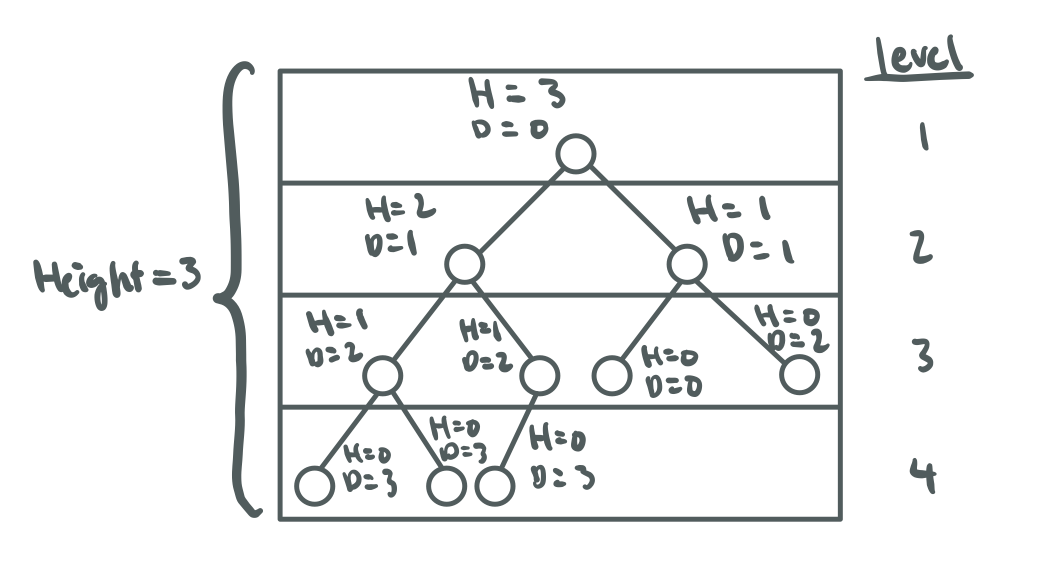
\includegraphics[width=\textwidth]{TreeDiagram.png}
    \end{center}
\end{figure}
%----Properties----%
\subsubsection{Properties}
\textbf{BST Properties}
\begin{itemize}
    \item Ordered tree where each node can have up to 2 children
    \item Called left and right children by convention
    \item \textbf{Full}
    \begin{itemize}
        \item Every node has either exactly 2 children or no children
    \end{itemize} 
    \item \textbf{Complete}
    \begin{itemize}
        \item Tree is filled at all levels except the last level
    \end{itemize} 
    \item \textbf{Perfect}
    \begin{itemize}
        \item It is full and all leaves are at the same level
    \end{itemize} 
\end{itemize}
\begin{figure}[H]
    \begin{center}
        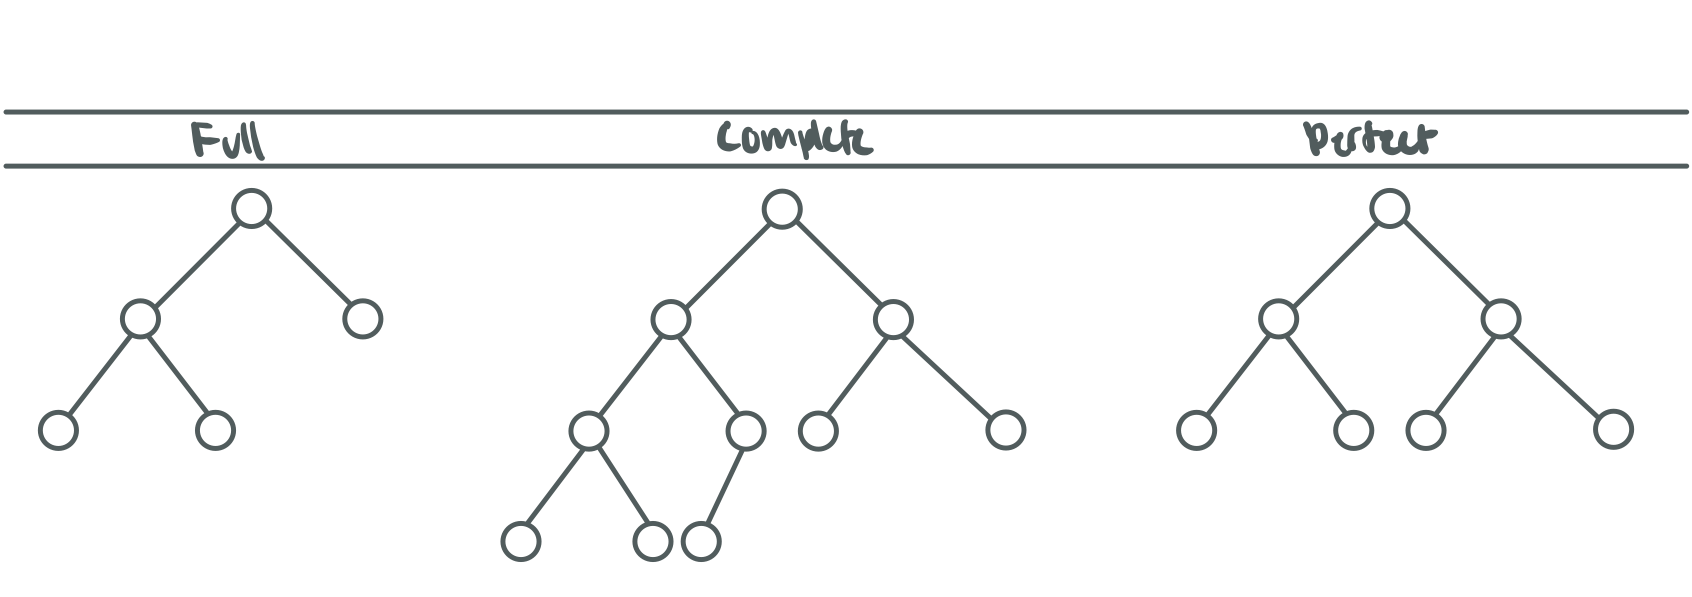
\includegraphics[width=\textwidth]{BSTTrees.png}
    \end{center}
\end{figure}
\textbf{Prove} that the Height of a Complete Tree is $O(\log(n))$
\begin{itemize}
    \item A complete tree of height h is perfect up to the height $h - 1$
    \item That is, h is $O(\log(n))$
    \item \textbf{Claim}: The height, h, of a complete tree with $n \geq 1$ nodes is $O(\log(n))$ 
    \begin{proof}
        \begin{itemize}
            \item Let $P(n)$ be the assertion that height, h, of a complete tree with n nodes is $O(log(n))$
            \item \textbf{Basis}: $P(1)$ A tree with 1 node, the root, has a height of $O(log(1))$
            \begin{itemize}
                \item This evaluates to $O(0)$ or simply a constant
                \item This is true because a single node tree has a height of 0
            \end{itemize}
            \item \textbf{Inductive Step}: Assume $P(k)$ holds for all k such that $1 \leq k < n$
            \begin{itemize}
                \item That is, any complete tree with k nodes has a height, $h = O(log(k))$
                \item Now, consider a complete tree with \textit{j} nodes. This tree can be divided into 2 parts:
                \begin{itemize}
                    \item A sub tree with $\frac{j}{2}$ nodes
                    \item Another tree with $\frac{j}{2}-1$ nodes
                \end{itemize}
                \item By the \textbf{inductive hypothesis}, the height of the sub tree with $\frac{j}{2}$ nodes is $O(\log(\frac{j}{2}))=O(\log(j))$
                \item The heigh of the subtree with $\frac{j}{2}-1$ nodes is $O(\log(\frac{j}{2}-1))=O(\log(j))$
                \item The height of the complete tree with j nodes is one more than the height of its taller sub tree
                \item Hence, he height of the complete tree is at most $O(log(j))$
            \end{itemize}
            \item Since the \textbf{basis} and the \textbf{inductive step} hold, the claim is established by mathematical induction
        \end{itemize}
    \end{proof}
\end{itemize}
\textbf{BST Traversal}
\begin{figure}[H]
    \begin{center}
        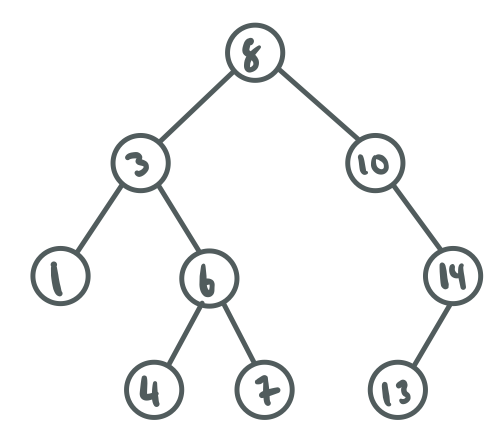
\includegraphics[width=0.5\textwidth]{BSTTraversal.png}
    \end{center}
\end{figure}
\begin{itemize}
    \item \textbf{In-Order}: 1, 3, 4, 6, 7, 10, 13, 14
    \begin{itemize}
        \item left subtree $\rightarrow$ root $\rightarrow$ right subtree
    \end{itemize}
    \item \textbf{Pre-Order}: 8, 3, 1, 6, 4, 7, 10, 14, 13
    \begin{itemize}
        \item root $\rightarrow$ left subtree $\rightarrow$ right subtree
    \end{itemize}
    \item \textbf{Post-Order}: 1, 4, 7, 6, 3, 13, 14, 10, 8
    \begin{itemize}
        \item left subtree $\rightarrow$ right subtree $\rightarrow$ root
    \end{itemize}
    \item \textbf{Predecessor}: The next node in an in-order traversal with the largest value that is smaller than the node itself
    \begin{itemize}
        \item e.g. 4 is the predecessor of 6, 1 is the predecessor of 3
        \item Comes immediately before in an in-order traversal
    \end{itemize} 
    \item \textbf{Successor}: The previous node in an in-order traversal with the smallest value that is greater than the node itself
    \begin{itemize}
        \item 7 is the successor of 6, 6 is the successor of 4
    \end{itemize}
\end{itemize}
%----Algorithm----%
\subsubsection{Algorithm}
\begin{lstlisting}
    // Search
    contains(T item, Node root) {
        if (root == null) {
            return false;
        } else if (item.compareTo(root.value) < 0) {
            return recContains(item, root.left);
        } else if (item.compareTo(root.value) > 0) {
            return recContains(item, root.right);
        } else {
            return true;
        }
    }
    // Insert
    recAdd(T item, Node root) {
        if (root == null) {
            root = new Node<T>();
            root.value = item;
        } else if (item.compareTo(root.value) < 0) {
            root.left = recAdd(item, root.left);
        } else {
            root.right = recAdd(item, root.right);
        }
        return root;
    }
    // Delete
    recRemove(T item) {
        if (root == null) {
            return null;
        } else if (item.compareTo(root.value) < 0) {
            root.left = recRemove(item, root.left);
        } else if (item.compareTo(root.value) > 0) {
            root.right = recRemove(item, root.right);
        } else {
            root = removeNode(root);
        }
        return root;
    }
    removeNode(Node<T> root) {
        T tmp;
        if (root.left == null) {
            return root.right;
        } else if (root.right == null) {
            return root.left;
        } else {
            tmp = predecessor(root.left);
            root.value = tmp;
            root.left = recRemove(tmp, root.left);
            return root;
        }
    }
\end{lstlisting}
%----Time Complexity----%
\subsubsection{Time Complexity}
\textbf{BST relative to Height}
\begin{center}
    \begin{tabular}{|c|c|}
        \hline
        \textbf{Operation} & \textbf{Complexity} \\
        \hline
        search() & $O(h)$ \\
        \hline
        insert() & $O(h)$ \\
        \hline
        delete() & $O(h)$ \\
        \hline
    \end{tabular}
\end{center}
\textbf{BST}
\begin{center}
    \begin{tabular}{|c|c|}
        \hline
        \textbf{Operation} & \textbf{Complexity} \\
        \hline
        search() & $O(n)$ \\
        \hline
        insert() & $O(n)$ \\
        \hline
        deleted() & $O(n)$ \\
        \hline
    \end{tabular}
\end{center}
\textbf{Balanced BST}
\begin{center}
    \begin{tabular}{|c|c|}
        \hline
        \textbf{Operation} & \textbf{Complexity} \\
        \hline
        search() & $O(\log(n))$ \\
        \hline
        insert() & $O(\log(n))$ \\
        \hline
        deleted() & $O(\log(n))$ \\
        \hline
    \end{tabular}
\end{center}
\newpage
%-----------------------------------------------------------------------------------%
%--Red and Black Trees--%
\subsection{Red and Black Trees}
%----Properties----%
\subsubsection{Properties}
A \textbf{red-black tree} is a concrete implementation of a \textbf{self-balancing binary-search tree} (reference here) that automatically maintains balance. 
Giving each node their respective color ensures that no path is more than twice as long as any other, thus is able to maintain approximate balance.\
\begin{enumerate}
    \item Every node is {\color{red}red}/black
    \item Root must be black
    \item Leaves (\textit{null}) are black
    \begin{itemize}
        \item \textit{null} vertices contain no values, while other (interior) do
    \end{itemize}
    \item If a node is {\color{red}red}, then both its children are black
    \item For each node, all simple paths from the node to descendant leaves contain the same number of black nodes 
\end{enumerate}
%----Lemma----%
The following \textbf{lemma} shows why red-black trees make good search trees:
\begin{lemma}
    A red-black tree with $n$ internal nodes has height at most $2\log (n+1)$
\end{lemma}
\begin{proof}
    Start by showing subtree rooted at any node $x$ contains at least a $2^{bh(x)}-1$ internal nodes. We prove this by \textbf{mathematical induction} on the height of $x$.
    \begin{description}
        \item [\textbf{Claim:}] If height of $x=0$, then the leaf must be \textit{T.null}, and the subtree rooted at $x$ contains at least $2^{bh(x)}-1=2^0-1=0$ internal nodes.
        \begin{description}
            \item \textbf{Inductive step:} 
            \begin{itemize}
                \item Consider a node $x$ that has positive height and is an internal node with two children.
                \item Each \textit{child} has a black-height of either $bh(x)$ or $bh(x)-1$ (depending on whether it is {\color{red}red} or black respectively).
                \item Since height of a \textit{child} of $x$ is less than the height of $x$ itself, we can apply the \textbf{I.H} to conlude that:
                \begin{itemize}
                    \item Each child has at least $2^{bh(x)-1}-1$ internal nodes.
                \end{itemize}
            \end{itemize}
            \item Thus, subtree rooted at $x$ contains at least $$(2^{bh(x)-1}-1)+(2^{bh(x)-1}-1)+1$$ internal nodes, which proves the claim.
        \end{description} 
        \item To complete the proof, let $h$ be the height of thr tree. According to property 4 (reference above Properties), at least half the nodes from the root 
        to a leaf (not including the root) must be black.
        \item Consequently, the $bh$ of the root must be at least $h/2$; thus, $$n \geq 2^{h/2}-1$$
        \item Moving $1$ to the left side and taking log on both sides yields: $$\log(n+1) \geq h/2$$ or $$h \leq 2\log(n+1)$$
    \end{description}
\end{proof}
\newpage
%----Rotations----%
\subsubsection{Rotational Properties}
Search operations \textit{TREE-INSERT} and \textit{TREE-DELETE} take $O(\log n)$ time. Since modifications are done to the tree, we must change the color of some of the nodes.
\begin{definition}[\textbf{Rotation}]
    Local operation that preserves the binary-tree property. 
    \begin{itemize}
        \item \textbf{Left Rotation:} assume that its right child $y$ is not \textit{null} 
        \item \textbf{Right Rotation:} assume that its left child $y$ is not \textit{null}
        \begin{itemize}
            \item $x$ can be any node on the tree whose respective child is not \textit{null}
            \item Left/Right rotations "pivots" around the link from $x$ to $y$
            \item Makes $y$ the new root, $x$ as $y$'s left(right) child, $y$'s left(right) child as $x$'s right(left) child
        \end{itemize}
        \item Both L/R rotates run in $O(1)$ time
        \item Only pointers are changed, all attributes in a node remain the same
    \end{itemize}
\end{definition}
\begin{algorithm}
    \caption{Left-Rotate($T,x$)}

    $x = y.right$ \tcp*{set y}
    $x.right = y.left$ \tcp*{Turn y's left subtree into $x$'s right subtree}
    \uIf{$y.left \neq T.null$}
        {$y.left.p = x$\;}
    $y.p = x.p$\;
    \uIf{$x.p == T.null$}
        {$T.root = y$\;}
    \uElseIf{$x == x.p.left$}
        {$x.p.left = y$\;}
    \uElse{$x.p.right = y$\;}
    $y.left = x$\;
    $x.p = y$\;
\end{algorithm}
\begin{figure}[H]
    \begin{center}
        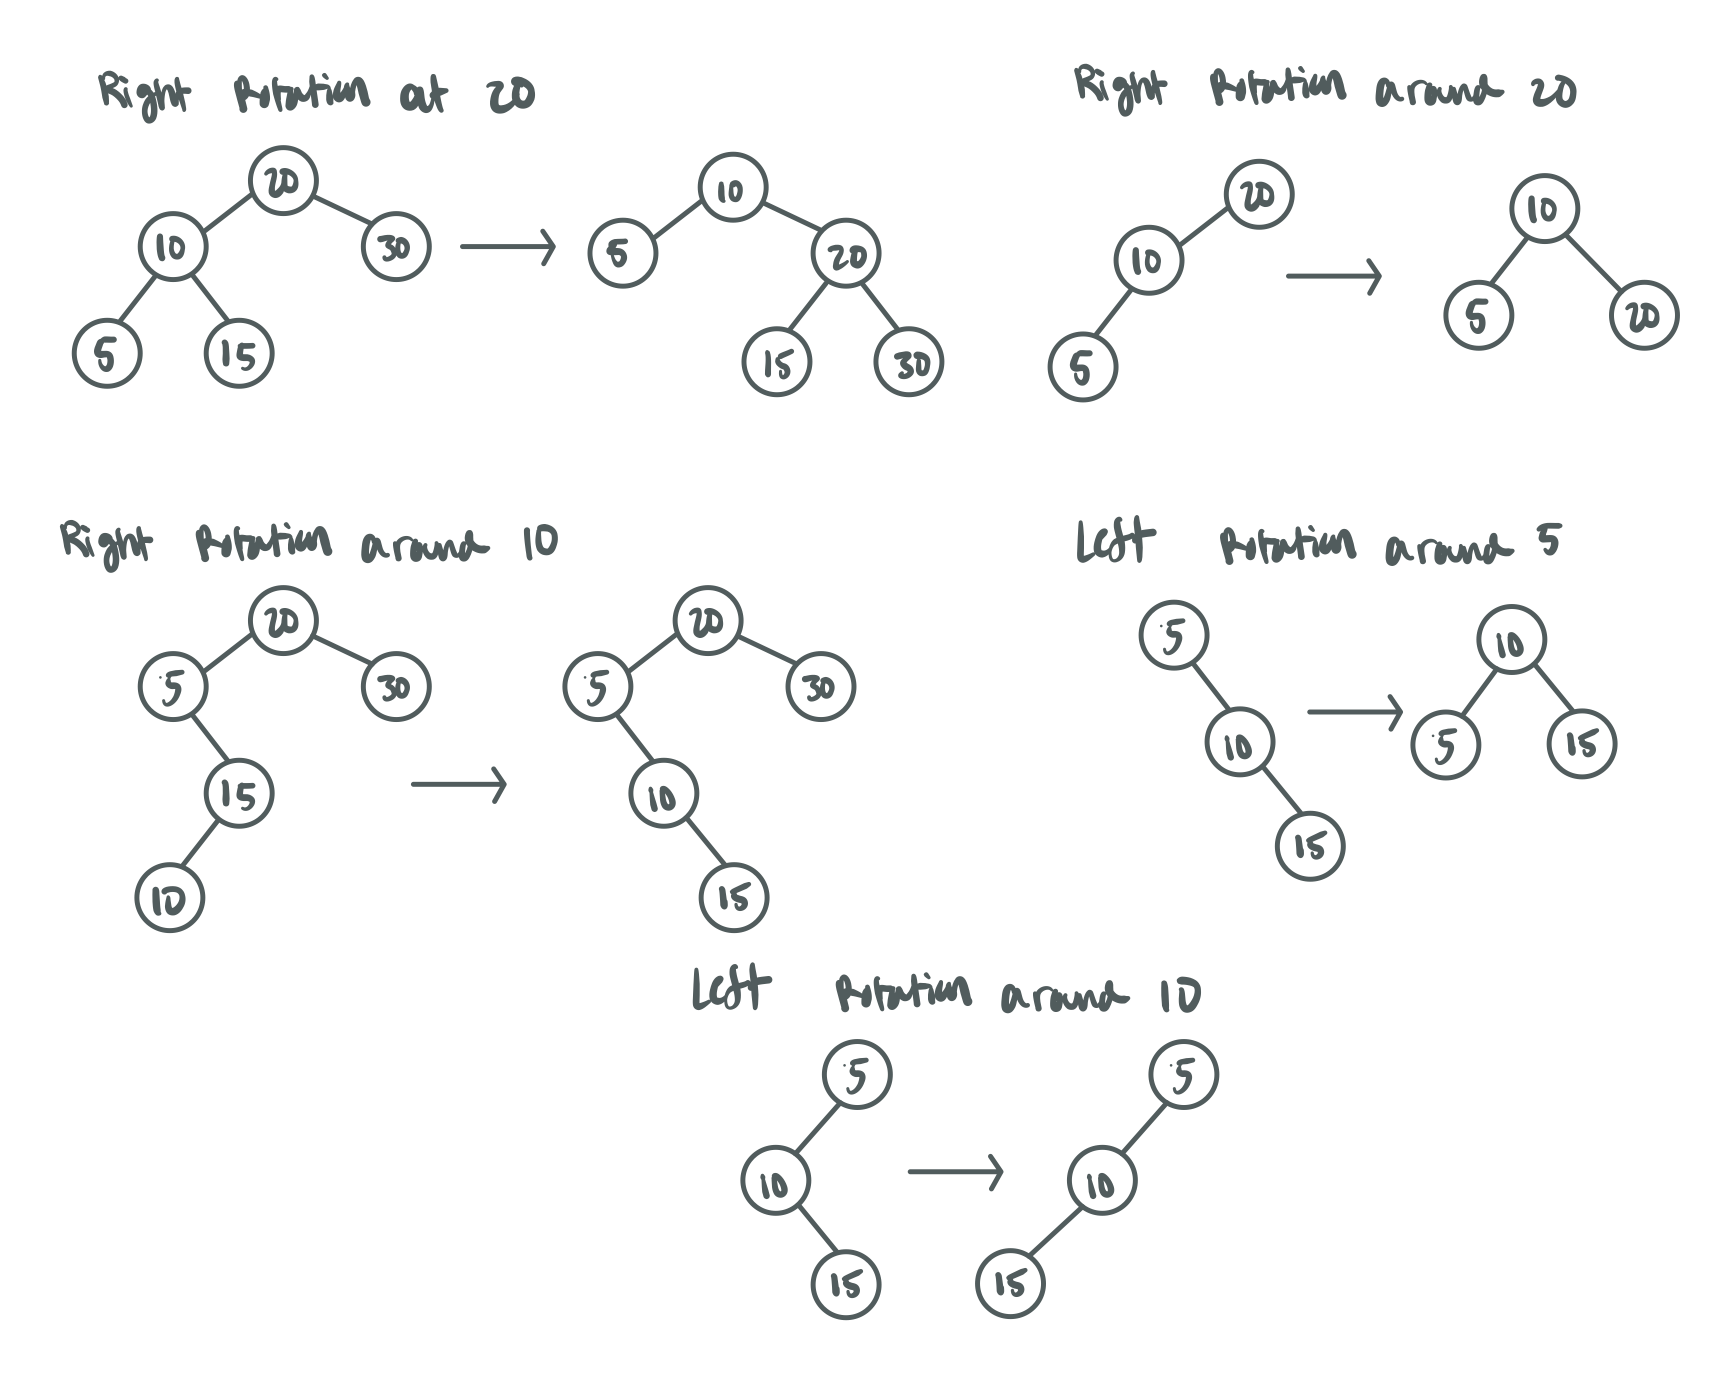
\includegraphics[width=0.72\textwidth]{RBRotation.png}
        \caption{DB Rotations}
    \end{center}
\end{figure}
%----Insertion----%
\subsubsection{Insertion}
\textbf{General Rules}:
\begin{enumerate}
    \item If tree is empty, insert node as root and color B
    \item If tree is \textbf{not} empty, insert new node as leaf and color R
    \item If Parent \textit{P} is B, exit
    \item Else if \textit{P} is R, check color of Uncle \textit{U}
    \begin{itemize}
        \item If \textit{U} is B/null, Rotate and Recolor
        \item If \textit{U} is R, Recolor and check Grandparent \textit{GP}
        \begin{itemize}
            \item If \textit{GP} is \textbf{not} root, Recolor and Recheck again
        \end{itemize}
    \end{itemize}
\end{enumerate}
\begin{itemize}
    \item If 3 nodes (e.g. A, B, C) are straight, coloring will involve the \textit{GP} and \textit{P} (that is, A and B) but \textbf{not} Node (C)
    \item For a path from GP$\rightarrow$P$\rightarrow$N:
    \begin{itemize}
        \item If it is left$\rightarrow$right or right$\rightarrow$left, follow the indicated rotations
        \item If nodes are straight with right$\rightarrow$right, left rotation 
        \item If nodes are straight with left$\rightarrow$left, right rotation 
    \end{itemize}
\end{itemize}
Inserting a node can be done in $O(\log n)$ time. Below is a pseudo-code that shows how insertion \textit{RB-INSERT} works:
\begin{algorithm}
    \caption{RB-INSERT$(T,z)$}
    \KwData{$z$ node to insert,}
    \BlankLine
    $y=T.null$\;
    $x=T.root$\;
    \While{$x \neq T.null$}
        {$y=x$\;        
        \eIf{$z.key < x.key$}
            {$x=x.left$\;}
        {$x=x.right$\;}}
    $z.p=y$\;
    \uIf{$y==T.null$}
        {$T.root=z$\;}
    \uElseIf{$z.key < y.key$}
        {$y.left=z$\;}
    \uElse{$y.right=z$\;}
    $z.left=T.null$\;
    $z.right=T.null$\;
    $z.color=T.RED$\;
    RB-INSERT$(T,z)$\;   
\end{algorithm}
\begin{figure}[H]
    \begin{center}
        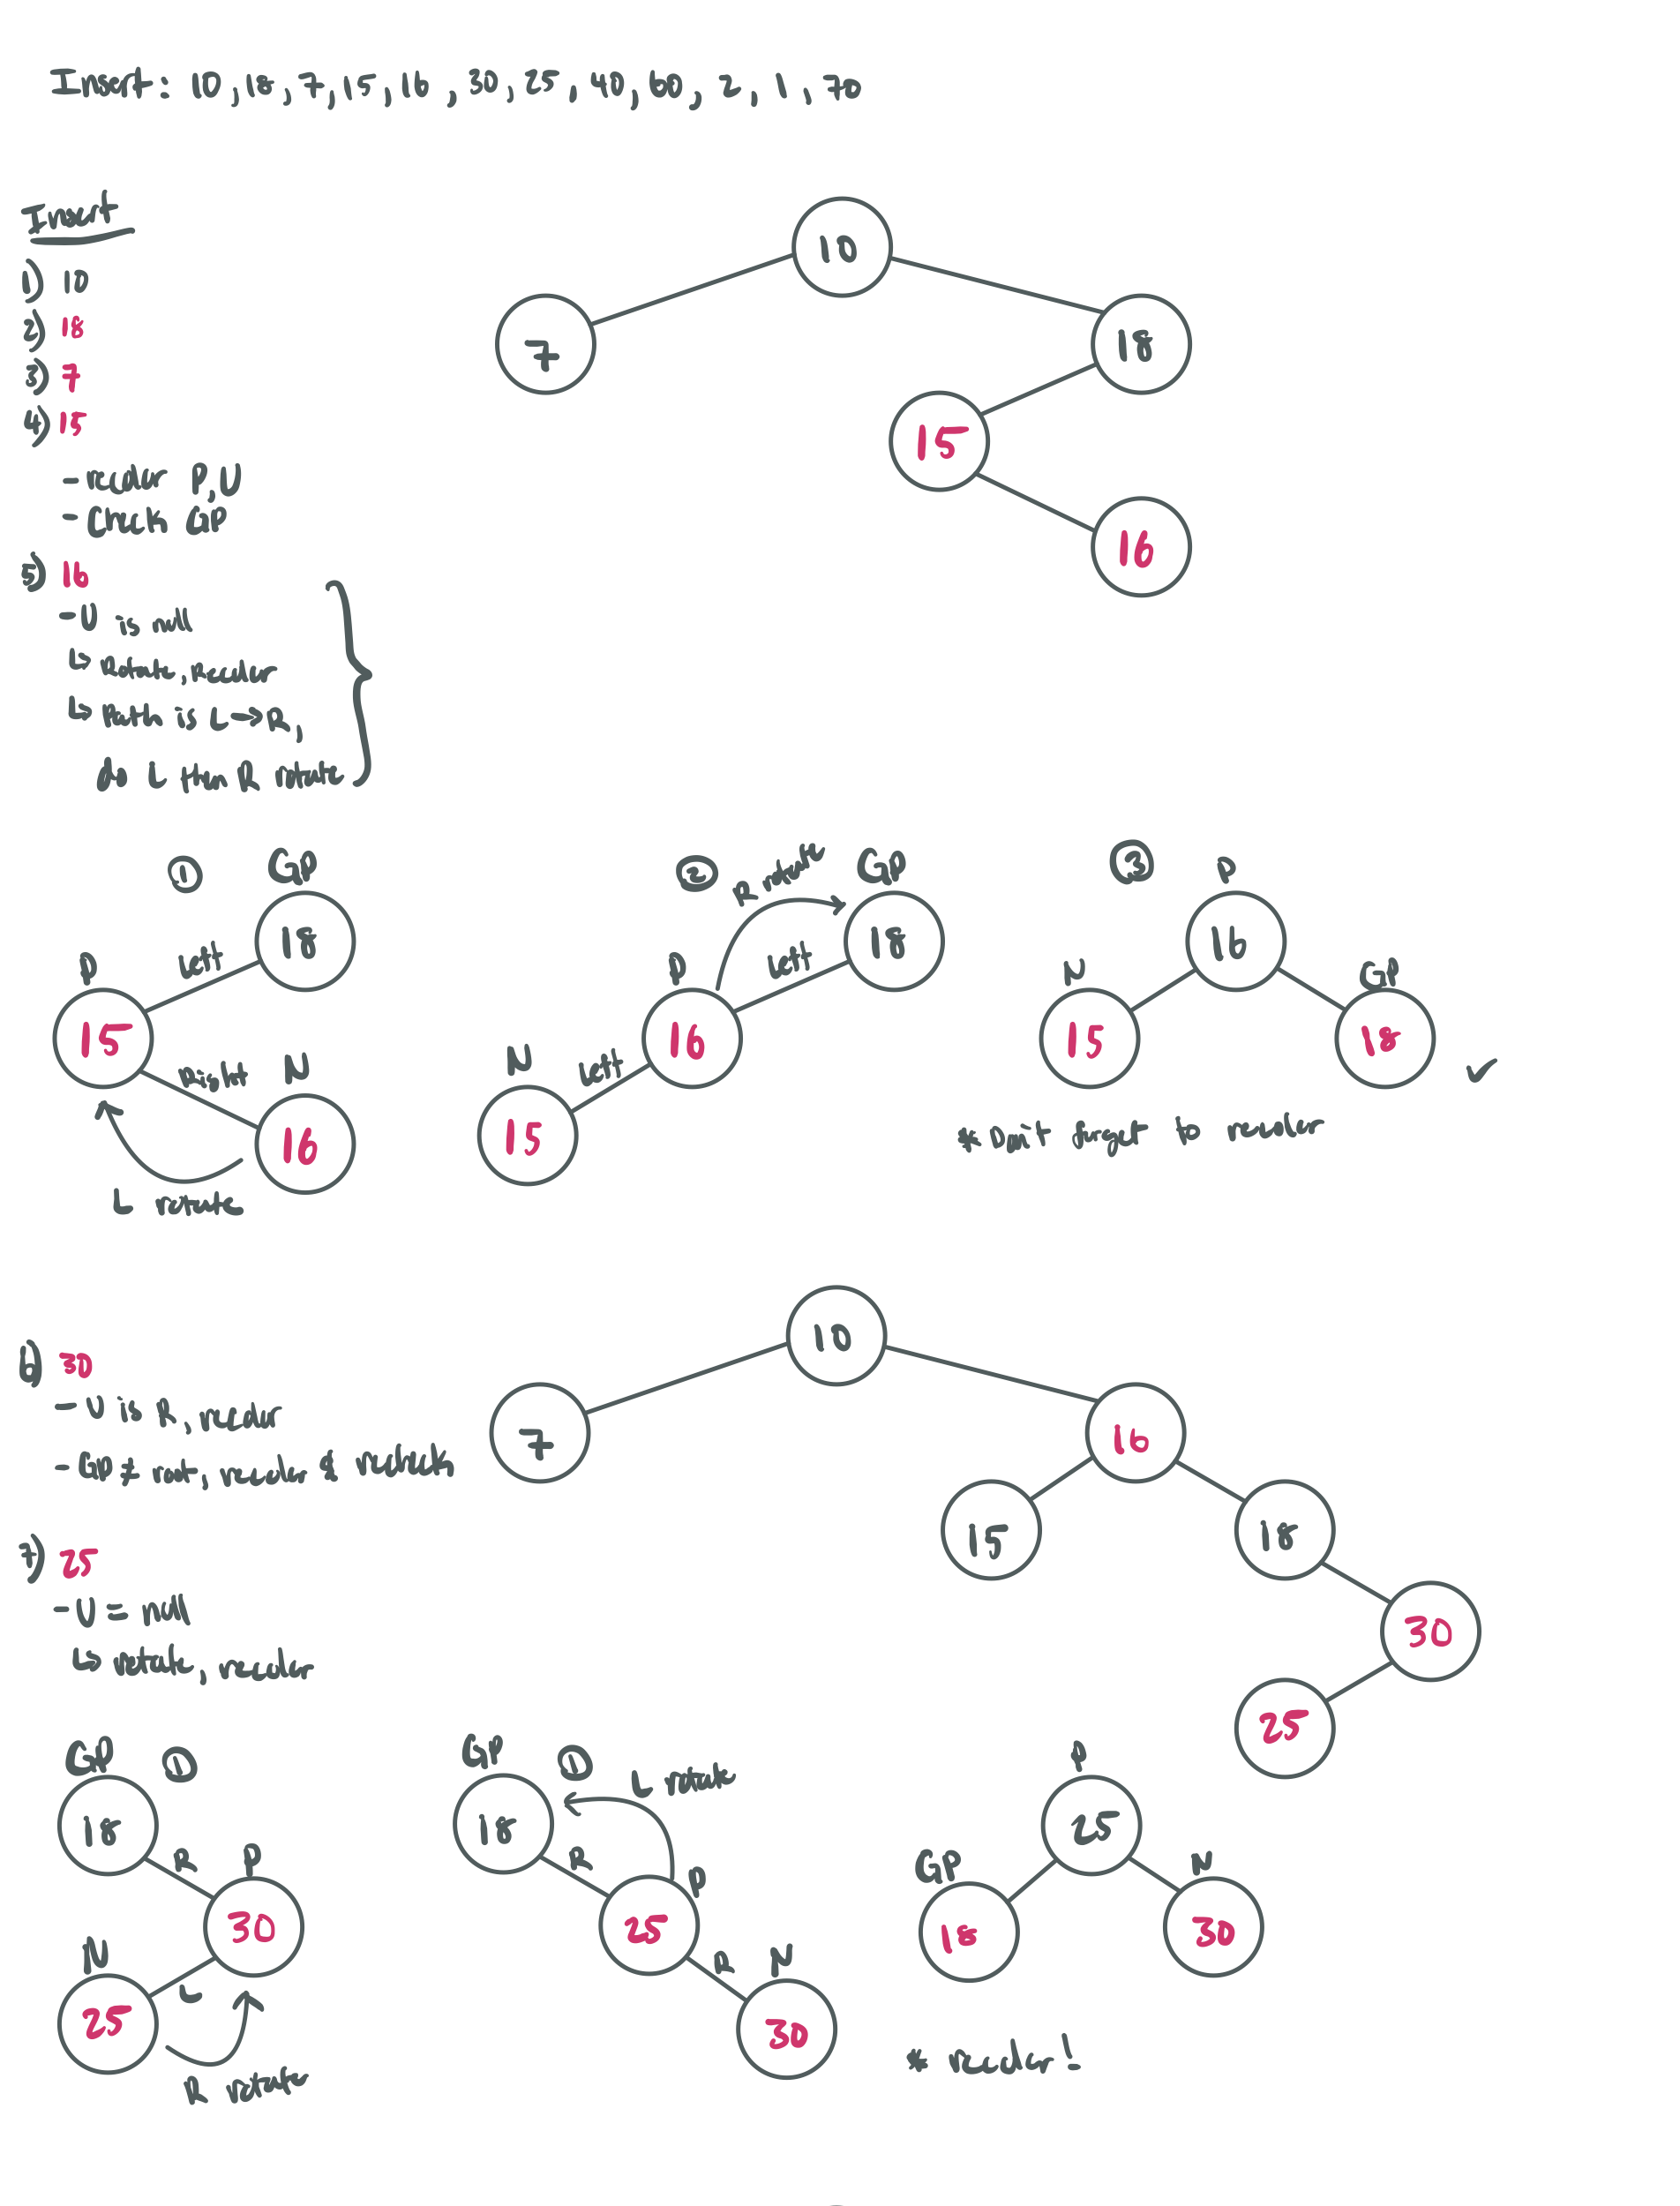
\includegraphics[width=\textwidth]{RBInsert1.png}
    \end{center}
\end{figure}
\begin{figure}[H]
    \begin{center}
        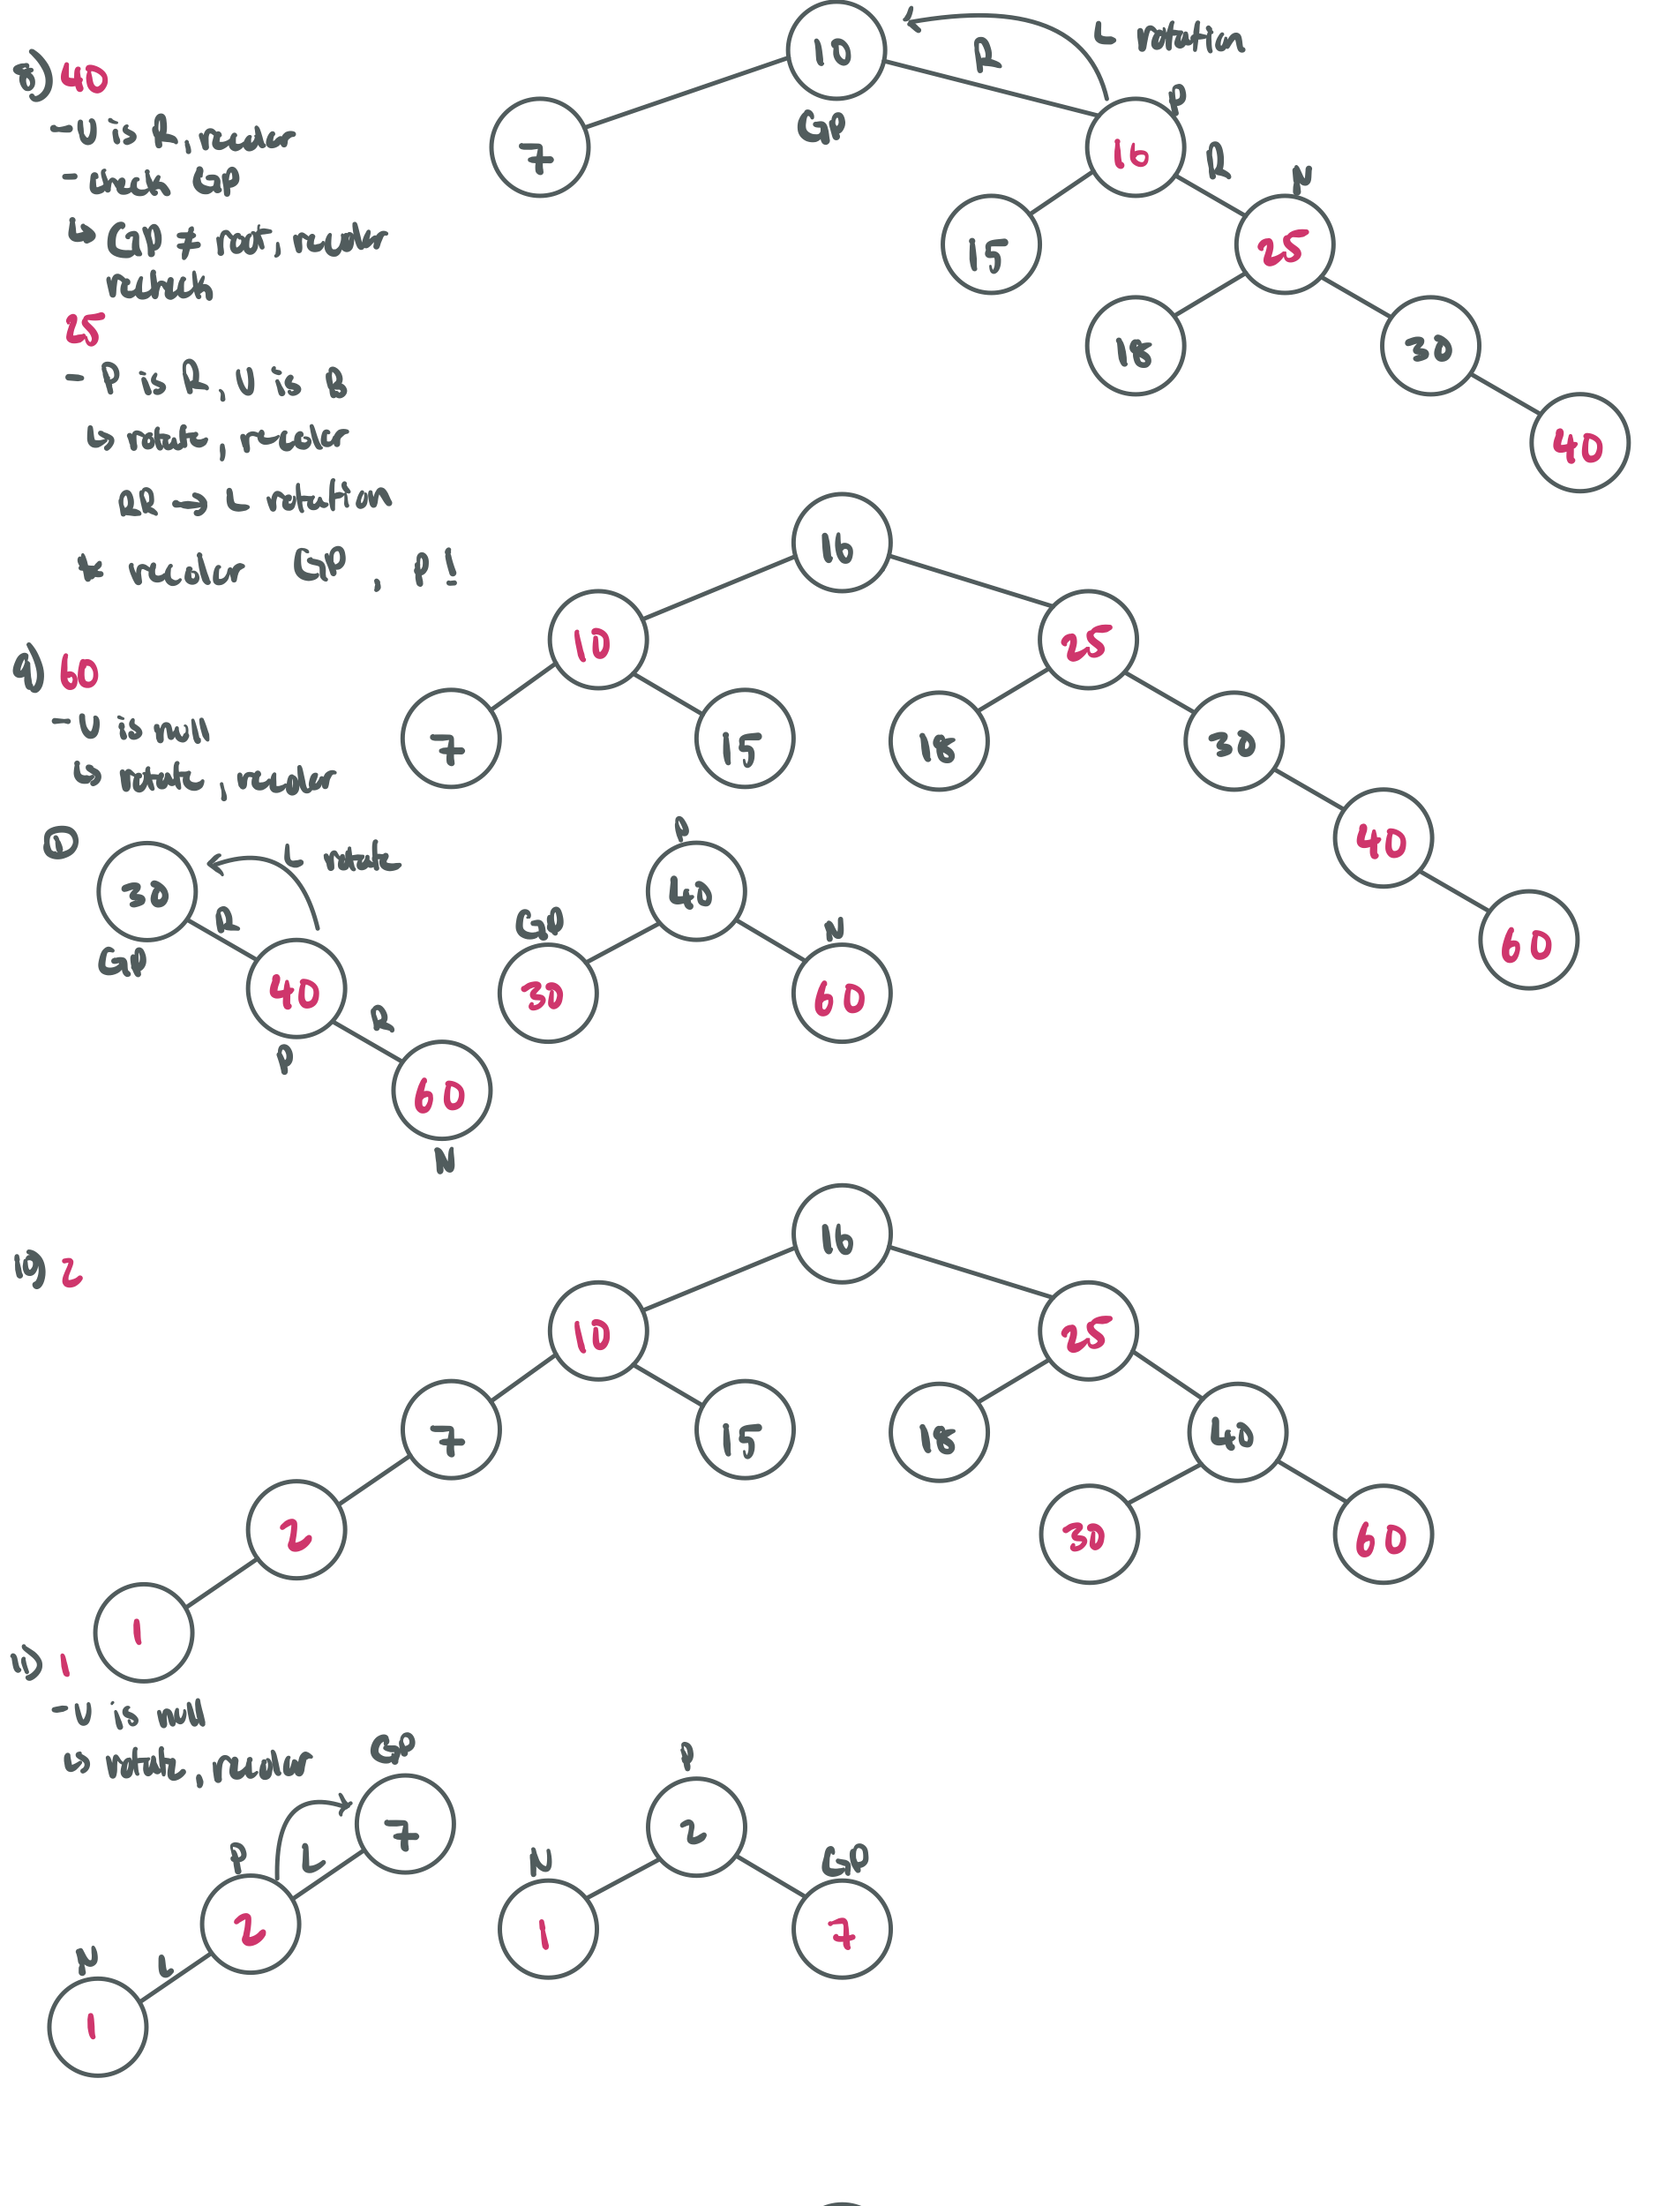
\includegraphics[width=\textwidth]{RBInsert2.png}
    \end{center}
\end{figure}
\begin{figure}[H]
    \begin{center}
        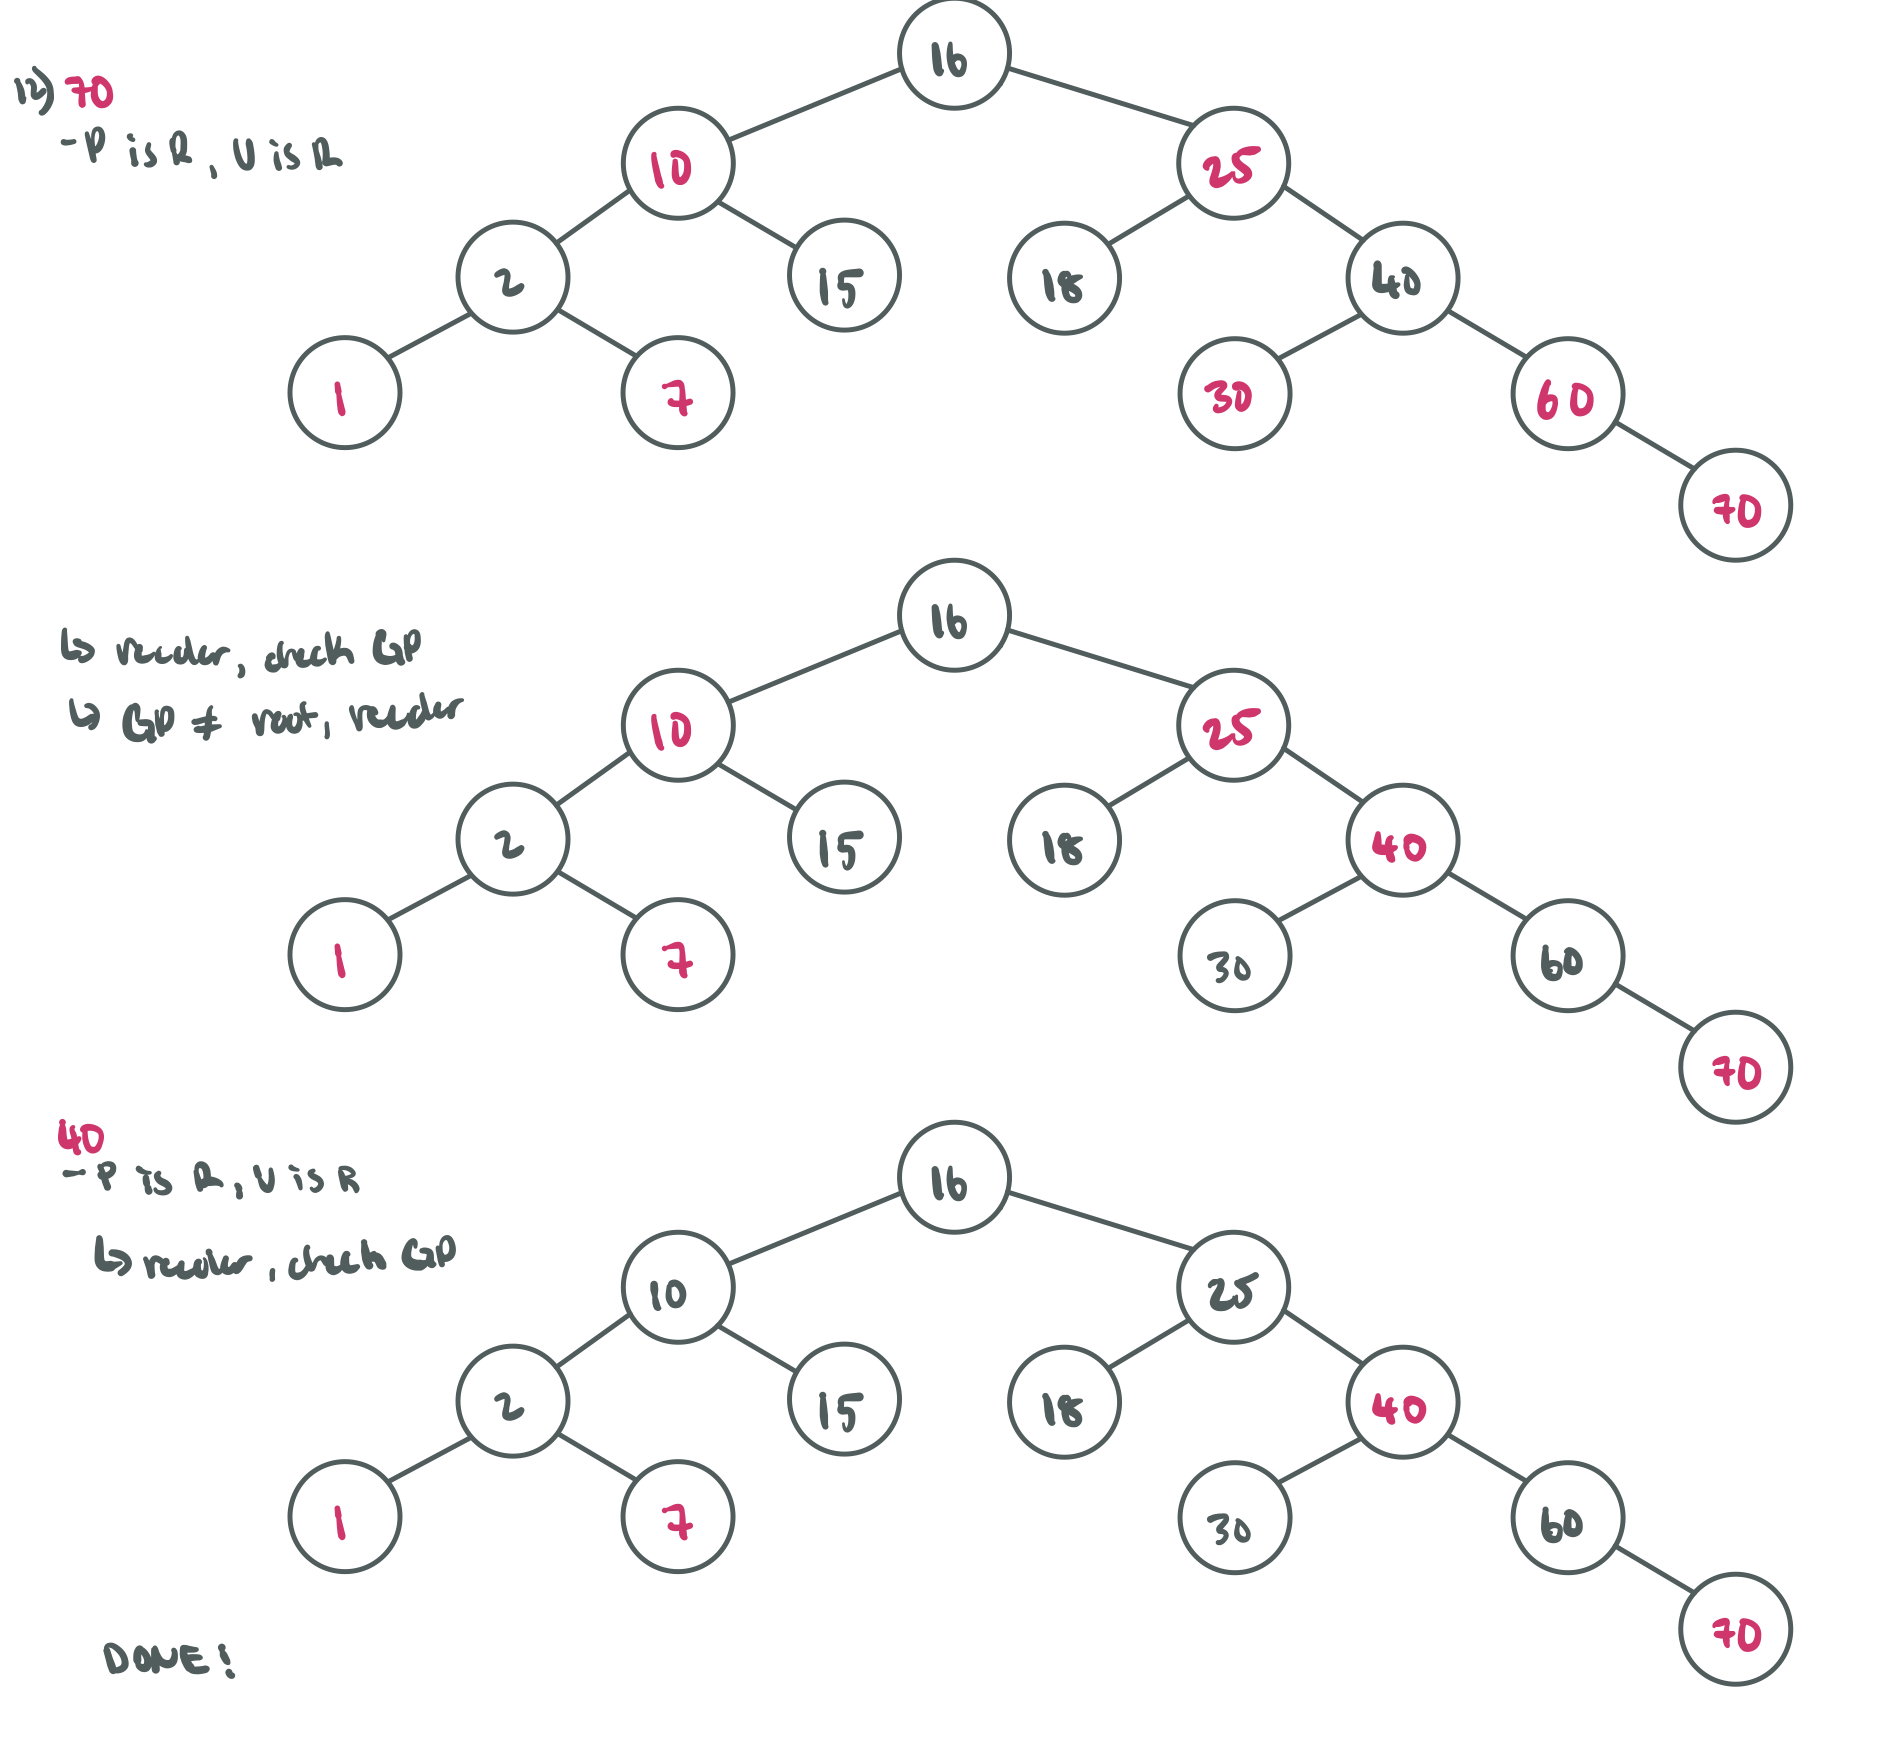
\includegraphics[width=\textwidth]{RBInsert3.png}
        \caption{Example of RBT Insert}
    \end{center}
\end{figure}
%----Correctness----%
\textbf{Correctness}
\begin{itemize}
    \item Add() function starts with the same method as the BST add(); thus resulting tree is still a BST
    \item Rotation functions do not change the BST property
    \item Prove that the rotations and coloring in fixAfterAdd() maintains the RBT Properties
\end{itemize}
%----Time Complexity----%
\textbf{Time Complexity}
\begin{itemize}
    \item Height of an RBT is $\leq 2\log(n+1)$, where \textit{n} is the number of values (non-null vertices) in the tree
    \item Adding a node is $O(\log n)$ W.C
\end{itemize}
\subsubsection{Deletion}
\textbf{6 Cases}
\begin{enumerate}
    \item If node is red \textit{r}, just delete
    \item If root is double black \textit{db}, just remove \textit{db}
    \item If \textit{db}'s sibling \textit{s} is black \textit{b} and both its children are \textit{b}
    \begin{itemize}
        \item Remove \textit{db}
        \item Add \textit{b} to its Parent \textit{p} (if \textit{r} becomes \textit{b}, else \textit{db})
        \item Make \textit{s} \textit{r}
        \item If \textit{db} still exists, apply other cases
    \end{itemize}
    \item If \textit{db} \textit{s} is \textit{r}
    \begin{itemize}
        \item Swap colors of \textit{p} and its \textit{s}
        \item Rotate \textit{p} in \textit{db} direction
        \item Reapply necessary cases
    \end{itemize}
    \item \textit{db}'s \textit{s} is \textit{b}, \textit{s} child far from \textit{db} is \textit{b}, but near child to \textit{db} is \textit{r}
    \begin{itemize}
        \item Swap color of \textit{db}'s \textit{s} and \textit{s} child who is near \textit{db}
        \item Rotate \textit{s} in opposite direction to \textit{db}'s direction
        \item Apply case 6
    \end{itemize} 
    \item \textit{db}'s \textit{s} is \textit{b}, far child is \textit{r}
    \begin{itemize}
        \item Swap color of \textit{p} and \textit{s}
        \item Rotate \textit{p} in \textit{db}'s direction
        \item Remove \textit{db}
        \item Change color of \textit{r} child to \textit{b}
    \end{itemize}
\end{enumerate}
%----Correctness----%
\textbf{Correctness}
\begin{itemize}
    \item Remove() function starts with the same method as the BST remove(); thus resulting tree is still a BST
    \item Rotation functions do not change the BST property
    \item Prove that the rotations and coloring in fixAfterRemove() maintains the RBT Properties
\end{itemize}
%----Time Complexity----%
\textbf{Time Complexity}
\begin{itemize}
    \item Height of an RBT is $\leq 2\log(n+1)$, where \textit{n} is the number of values (non-null vertices) in the tree
    \item Removing a node is $O(\log n)$ W.C
\end{itemize}
\newpage
%-----------------------------------------------------------------------------------%
%--Heaps--%
\subsection{Heaps}
%----Priority Queues----%
\subsubsection{Priority Queues} \label{subsubsec:prio-q}
\begin{itemize}
    \item Priority queues are \textbf{NOT} FIFO
    \item These queues are interested in removing items (dequeue) with the \textbf{highest priority}
    \item Assume that higher priority value (HPV) entails higher priority
    \begin{itemize}
        \item Not true in general (UNIX OS; smaller PV = higher priority)
    \end{itemize}
    \item Similar operations as the standard Queue ADT:
\end{itemize}
\begin{lstlisting}
    // Queue ADT
    public interface QueueADT<T> {
        public void enqueue(T item);
        public T dequeue(); // different implementation
        public boolean isEmpty();
        public boolean isFull();
    }
\end{lstlisting}
\BlankLine
\paragraph{\textbf{Priority Queue Implementations}}
\begin{itemize}
    \item \textbf{Lists}
    \begin{itemize}
        \item \textbf{Sorted} list by PV with \underbar{array implementation}
        \begin{itemize}
            \item \textit{Ascending order}: Remove \textbf{last} item
            \item \textit{Dequeue}: $O(1)$, \textit{n\textsuperscript{th}} element of the array to be removed
            \item \textit{Enqueue}: $O(n)$, needs to be sorted after enqueue
        \end{itemize}
        \item \textbf{Sorted} list by PV with \underbar{linked-list implementation} 
        \begin{itemize}
            \item \textit{Descending order}: Remove \textbf{first} item
            \item \textit{Ascending order}: Circular list implementation
            \item \textit{Dequeue}: $O(1)$
            \item \textit{Enqueue}: $O(n)$
        \end{itemize}
        \item \textbf{Unsorted} list
        \begin{itemize}
            \item \textit{Dequeue}: $O(n)$
            \item \textit{Enqueue}: $O(1)$
        \end{itemize}
    \end{itemize}
    \item \textbf{BST}
    \begin{itemize}
        \item \textit{Dequeue}: $O(\log(n))$ average-case, $O(n)$ worst-case 
        \item \textit{Enqueue}: $O(\log(n))$ average-case, $O(n)$ worst-case 
    \end{itemize}
    \item \textbf{Heaps}
    \begin{itemize}
        \item \textit{Dequeue}: $O(\log(n))$ worst-case 
        \item \textit{Enqueue}: $O(\log(n))$ worst-case 
    \end{itemize}
\end{itemize}
\newpage
%----Properties----%
\subsubsection{Properties}
A heap is a \textbf{complete} binary tree that satisfies the Heap Property:
\begin{itemize}
    \item Each node of a tree corresponds to an element of an array
    \begin{itemize}
        \item Always stored \textbf{contiguously}
        \begin{itemize}
            \item  If there are blanks, they are on the rightside of the array
            \item  Otherwise, no blanks inbetween indices
        \end{itemize}
    \end{itemize}
    \item It is of height \textit{h} and contains \textit{n} nodes
\end{itemize}
\begin{proof}
    Height \textit{h}
\end{proof}
\BlankLine
\paragraph{\textbf{Heap Properties}} (Figure \vref{fig:heap})
\label{heapproperties}
\begin{itemize}
    \item \textbf{Min Heap Property} 
    \begin{itemize}
        \item Every node has a value $\leq$ than the value of its children
        \item Root of any subtree has the \textit{minimum} value in the subtree    
    \end{itemize}
    \item \textbf{Max Heap Property}
    \begin{itemize}
        \item Every node has a value $\geq$ than the value of its children
        \item Root of any subtree has the \textit{maximum} value in the subtree
    \end{itemize}
    \item \textbf{Child-to-Parent Relation}
    \begin{itemize}
        \item Given a \textbf{child} a location \textit{loc}, what is the index of \textbf{parent} \textit{parent}?
        \item If Child is right, index is \textbf{even}
        \begin{itemize}
            \item $loc_r = 2 \times parent + 2$
        \end{itemize} 
        \item If Child is left, index is \textbf{odd}
        \begin{itemize}
            \item $loc_l = 2 \times parent + 1$
        \end{itemize}
        \item In either cases, $parent = (loc - 1) \div 2$
    \end{itemize}
\end{itemize}
\begin{figure}[H]
    \begin{center}
        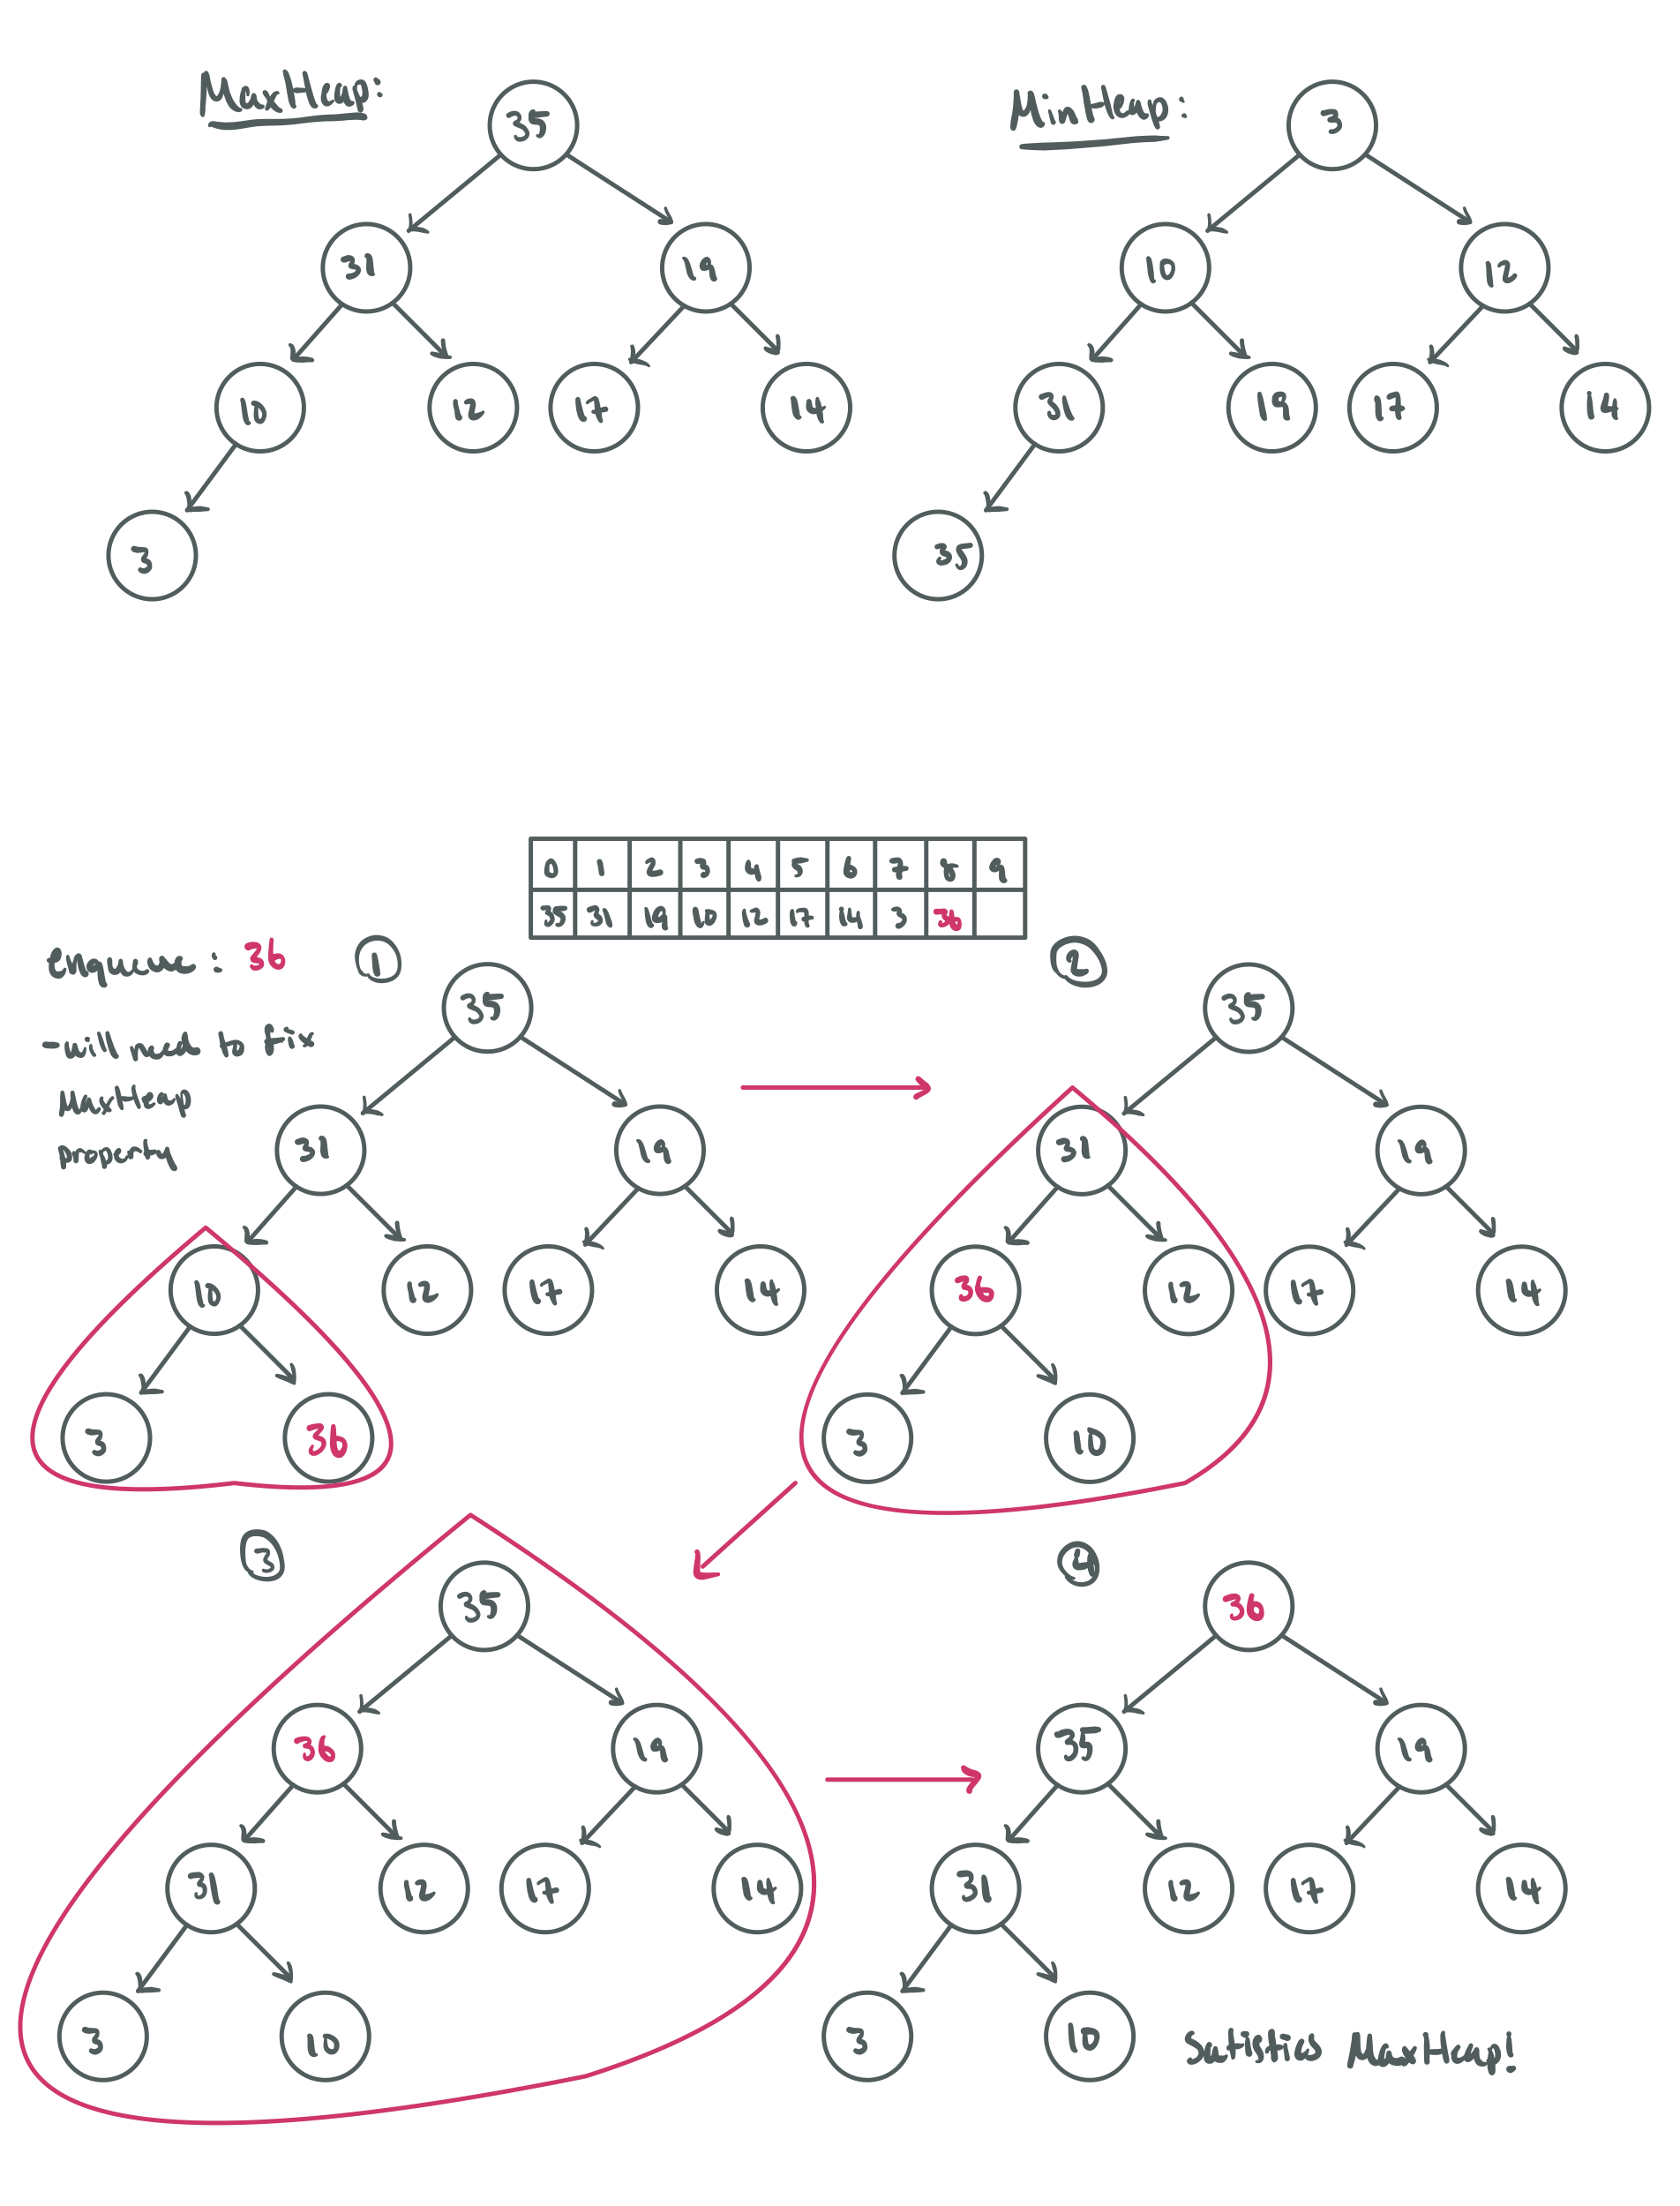
\includegraphics[width=\textwidth]{HeapDiagram.png}
        \caption{MaxHeap/MinHeap Diagram (\vref{heapproperties})}
        \label{fig:heap}
    \end{center}
\end{figure}
%----MaxHeap Class----%
\paragraph{\textbf{MaxHeap Class}}
Similar to the Queue ADT, differences in the enqueue and dequeue functions to maintain \textbf{heap} property
\begin{lstlisting}
    public class MaxHeap<T> {
        private T[] queue;
        private int size;

        public MaxHeap(Class<T> clazz, int maxSize) {
            queue = (T[]) Array.newInstance(clazz, maxSize);
            size = 0;
        }
        public boolean isEmpty() {
            return (size == 0);
        }
        public boolean isFull() {
            return (size == queue.length);
        }
    }
    // enqueue()/dequeue() functions shown later
\end{lstlisting}
%----Enqueue----%
\subsubsection{Insertion}
\begin{definition}
    Inserting an element (Figure \vref{fig:heapenq})
    \begin{itemize}
        \item Must keep the tree \textbf{complete}
        \item Must keep the \textbf{max heap} property
        \item \textbf{Complexity of \textit{Enqueue}}
        \begin{itemize}
            \item \textit{Worst-case}: added node percolates from leaf to root
            \item Since the tree is \textbf{complete}, height is $O(\log(n))$
            \item Hence, \textbf{enqueue} is $O(\log(n))$
        \end{itemize}
    \end{itemize}
\end{definition}
Enqueue:
\begin{lstlisting}
    public void enqueue(T item) {
        queue[size] = item;

        // Fix heap
        int loc = size;
        int parent = (loc - 1)/2;
        while (loc > 0 && queue[loc].compareTo(queue[parent]) > 0) {
            swap(loc, parent);
            loc = parent;
            parent = (loc - 1)/2;
        }
        size++;
    }
\end{lstlisting}
\begin{figure}[H]
    \begin{center}
        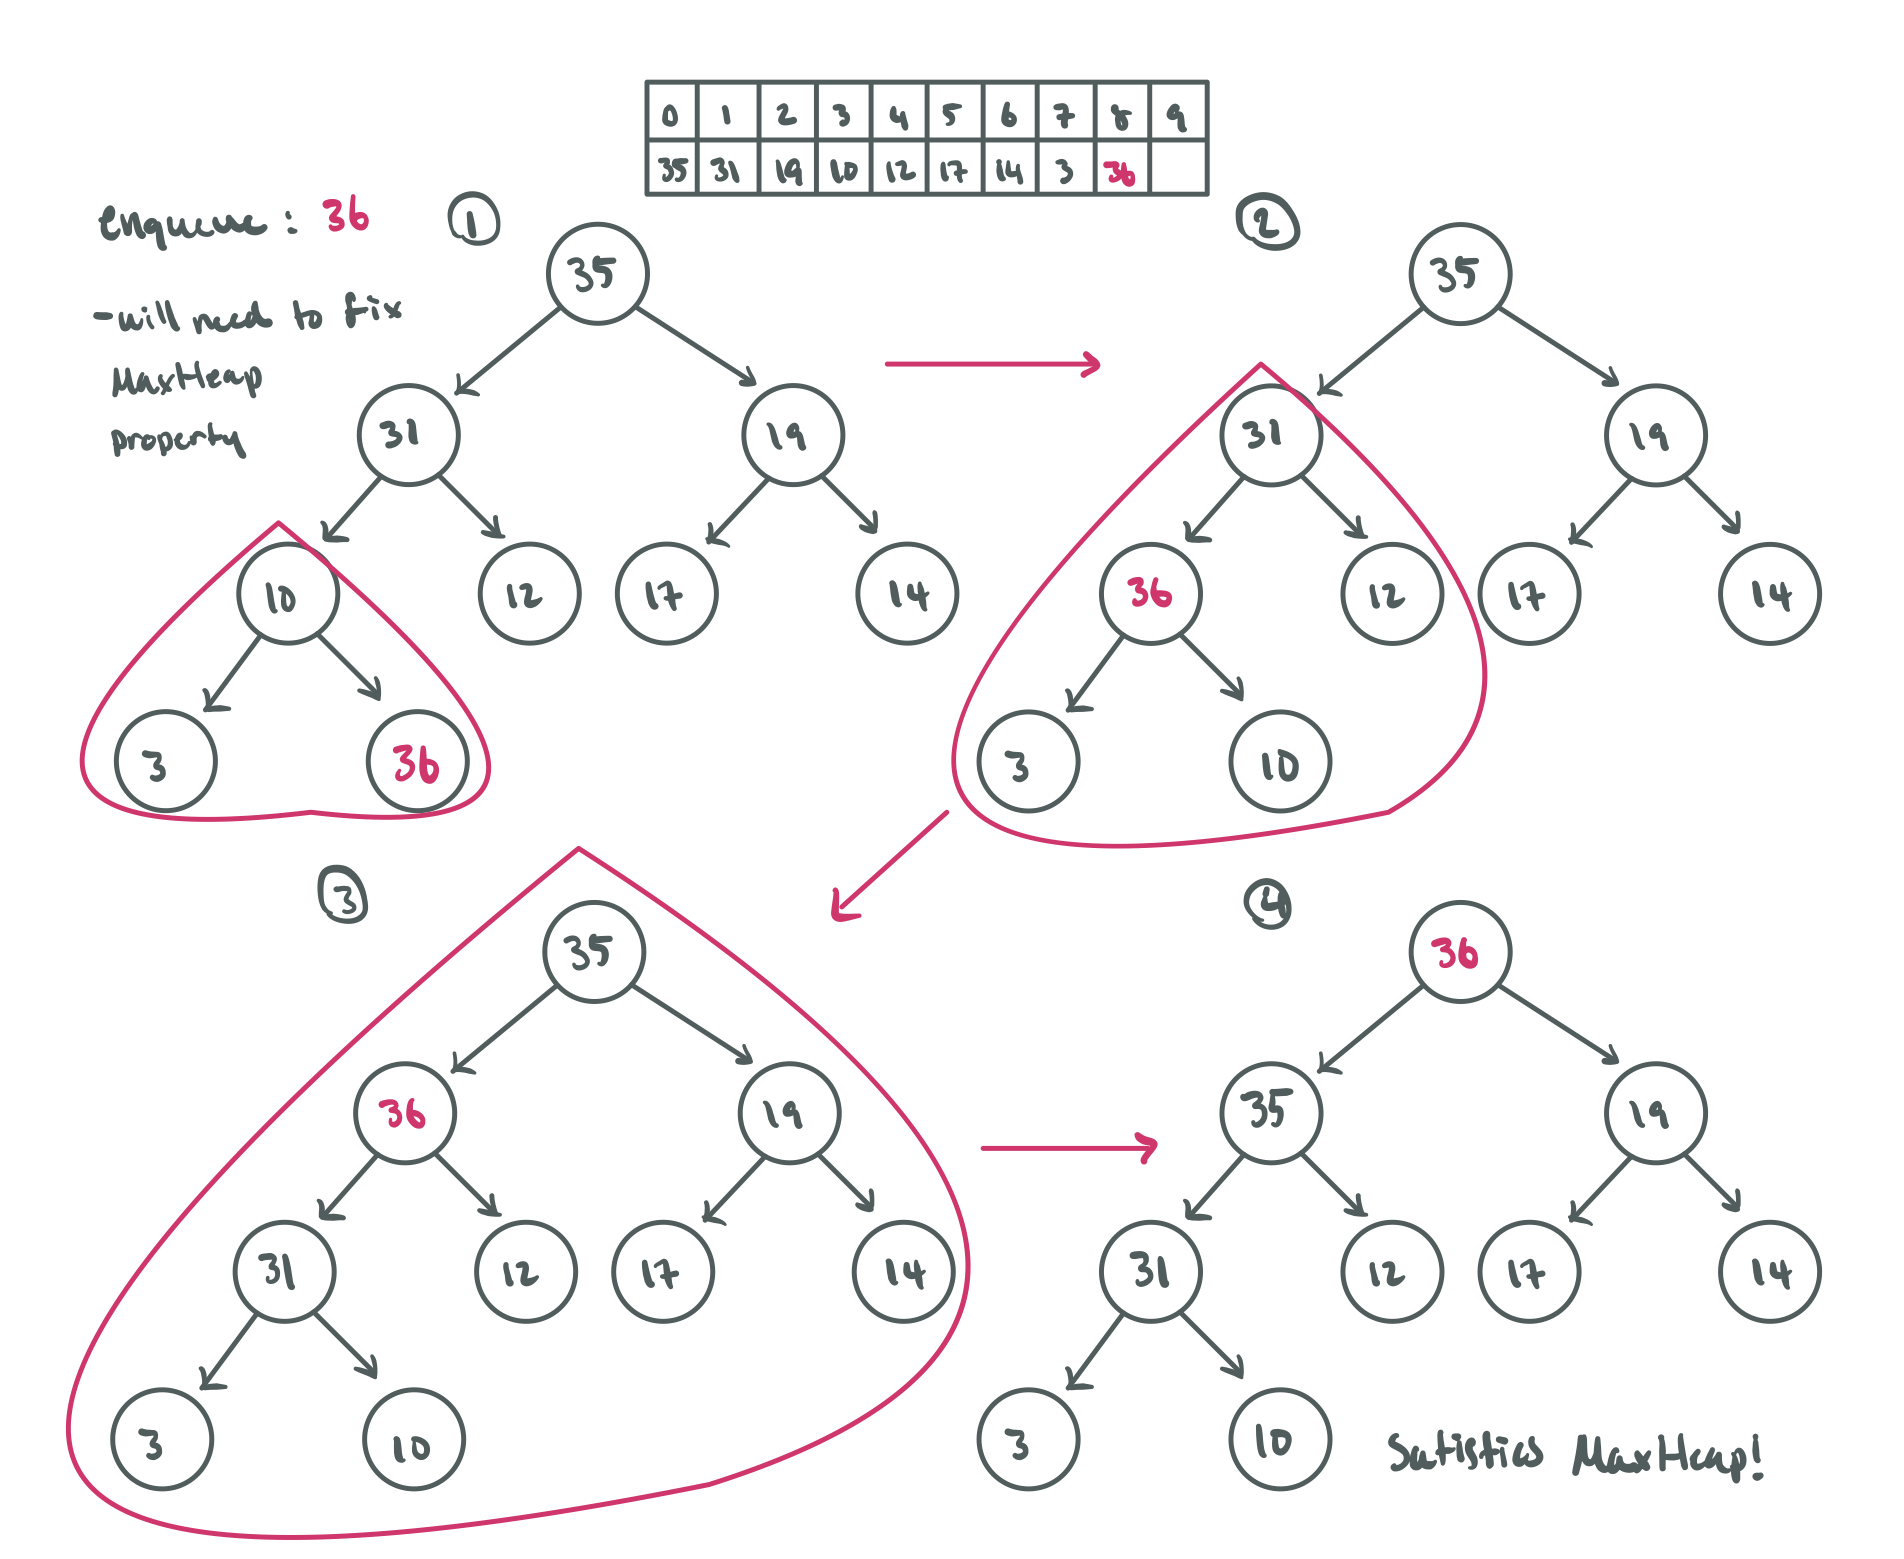
\includegraphics[width=0.9\textwidth]{HeapEnqueue.png}
        \caption{MaxHeap: Enqueue}
        \label{fig:heapenq}
    \end{center}
\end{figure}
Correctness: \textbf{Loop Invariant} for Enqueue
\begin{proof}
        
\end{proof}
\newpage
%----Dequeue----%
\subsubsection{Deletion}
\begin{definition}
    Deleting an element (Figure \vref{fig:heapdeq})
    \begin{itemize}
        \item Must keep the tree \textbf{complete}
        \item Must keep the \textbf{max heap} property 
        \item This process is called \textit{sinking}, where the leaf moves to location (index) 0
        \item We then \textit{sink} the leaf back to its respective location
        \item \textbf{Complexity of \textit{Dequeue}}
        \begin{itemize}
            \item Deleted root "hole" always sinks to a leaf
            \item Since the tree is complete, height is $O(\log(n))$
            \item Hence, \textbf{dequeue} is $O(\log(n))$
        \end{itemize}
    \end{itemize}
\end{definition}
Dequeue
\begin{lstlisting}
    public T dequeue() {
        T max = queue[0];
        queue[0] = queue[size - 1];
        sink(0);
        queue[size - 1] = null;
        size--;
        return max;
     }
\end{lstlisting}
Sink
\begin{lstlisting}
    int swapWith
    int left = 2*loc + 1;
    int right = 2*loc + 2;
    T tmp = queue[loc];

    if (left > (size - 1)) { return;} // Reached a leaf
    else if (left == size - 1) { // Node with one child
        if (tmp.compareTo(queue[left] < 0)) {
            swap(loc, left);
        }
    } else { // Node with two children
        if (queue[left].compareTo(queue[right]) < 0) {
            swapWith = right;
        } else {
            swapWith = left;
        } 
        if (tmp.compareTo(queue[left]) < 0) {
            swap(loc, swapWith);
        }
        sink(swapWith);
    }
\end{lstlisting}
\begin{figure}[H]
    \begin{center}
        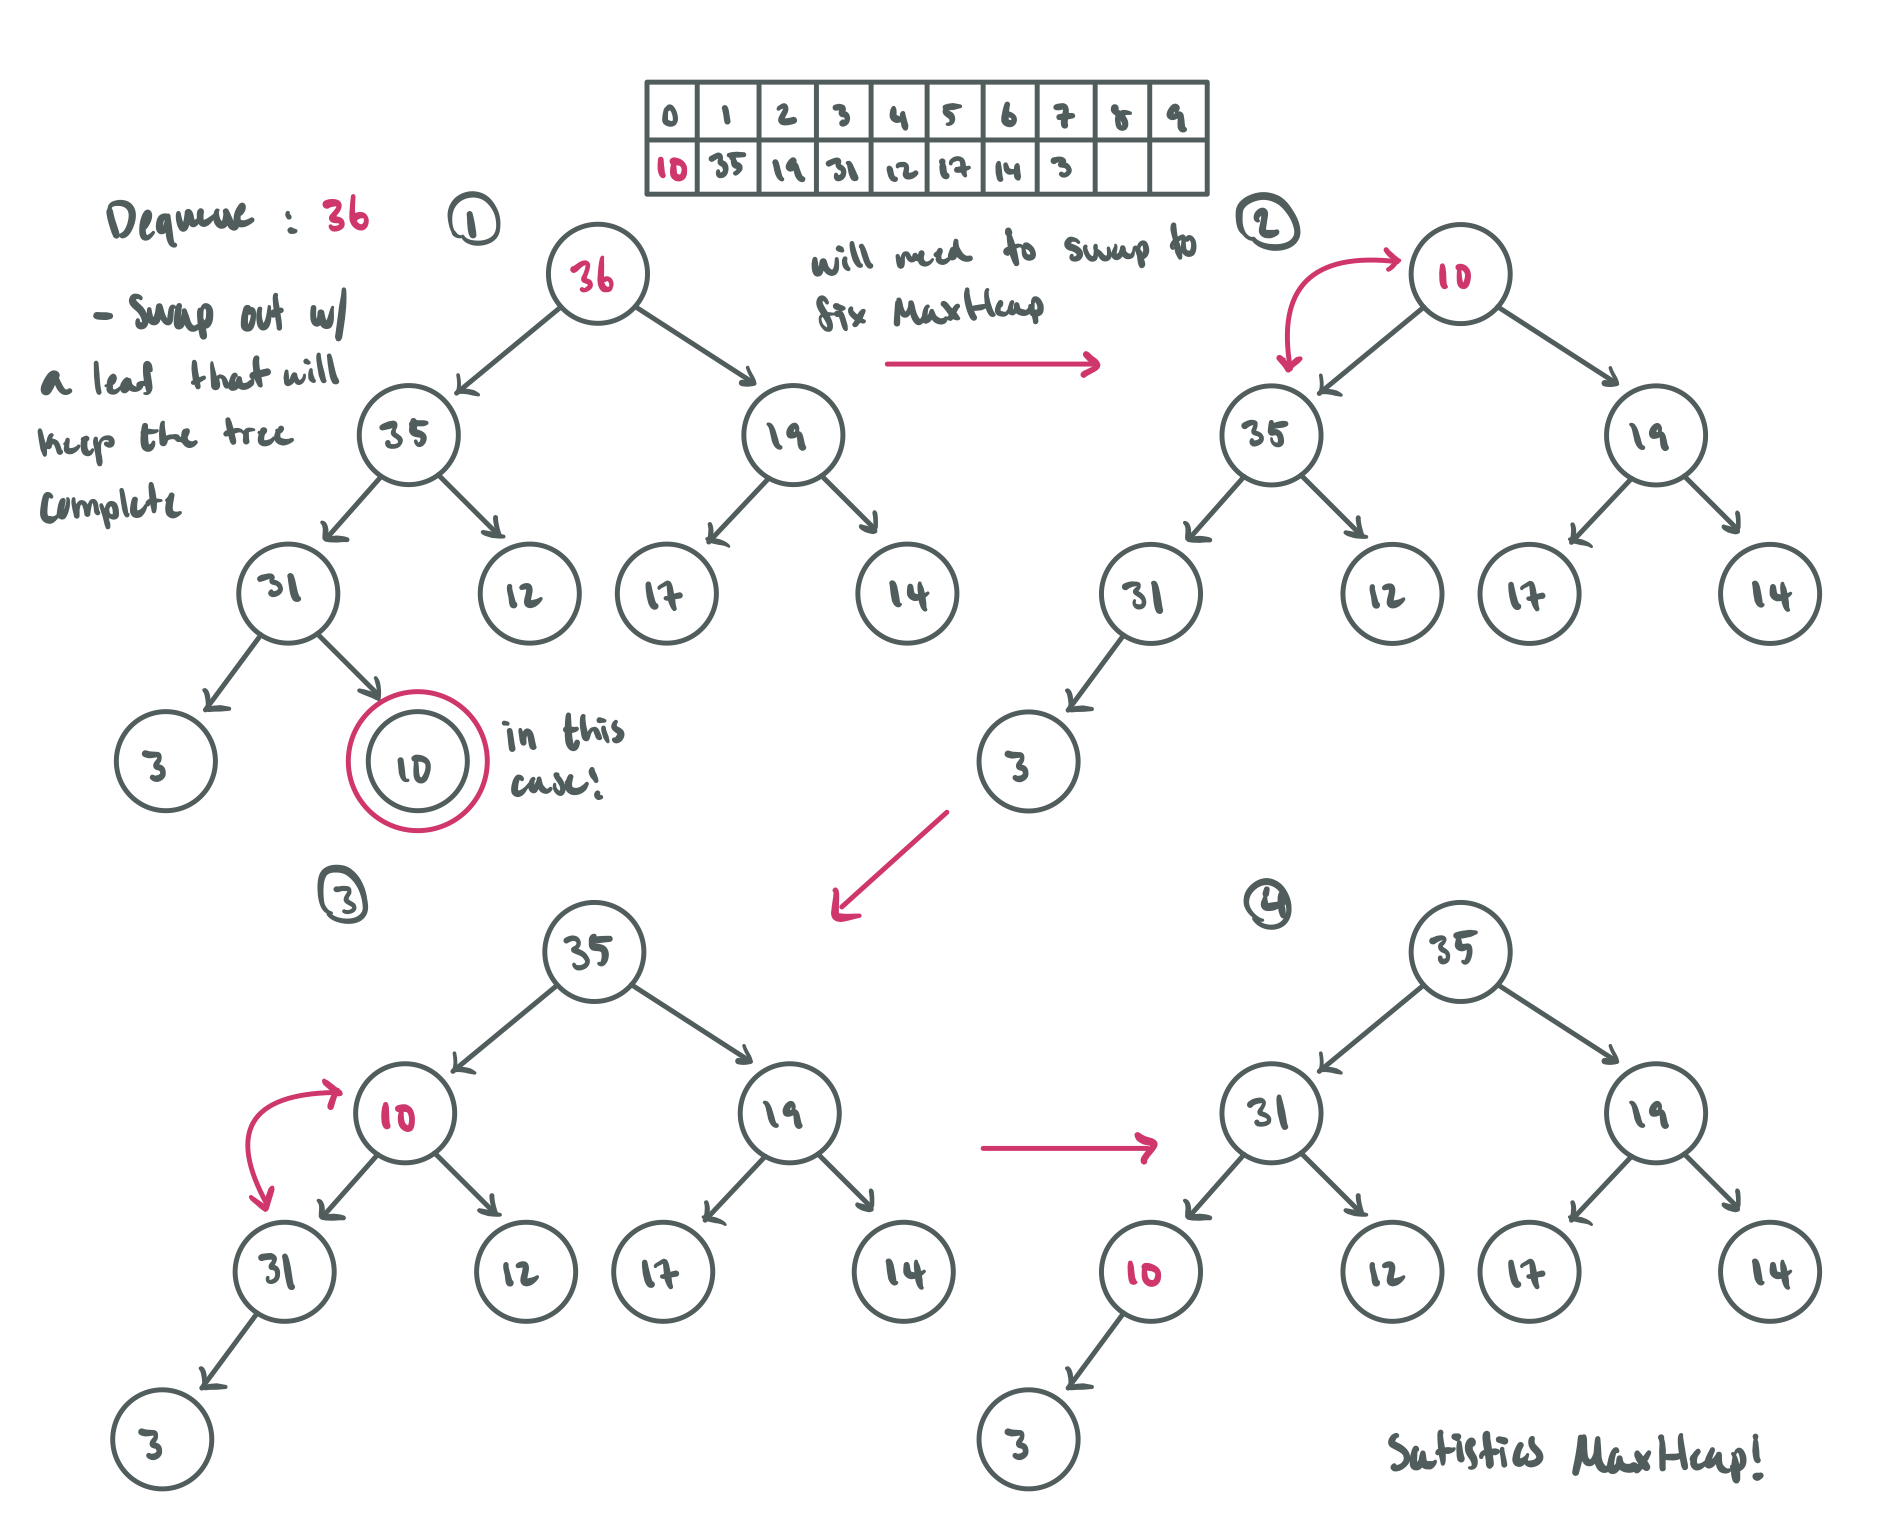
\includegraphics[width=\textwidth]{HeapDequeue.png}
        \caption{MaxHeap: Dequeue}
        \label{fig:heapdeq}
    \end{center}
\end{figure}
Correctness: \textbf{Bound Function} for Dequeue
\begin{proof}
    Prove that sink() maintains heap property
\end{proof}
\newpage
%-----------------------------------------------------------------------------------%
%--Hash Table--%
\subsection{Hash Table}
%----Properties----%
\subsubsection{Properties}
\begin{definition}
    \textit{Hash Table ADT}
    \begin{itemize}
        \item Allows adding, removing, searching for items in $O(1)$ on average
        \item Implementation is called \textit{hashing}
        \item Objects are mapped to a hash table based on a value calculated by a \textbf{hash function}
        using an object's key
        \begin{itemize}
            \item e.g. ID of a Student object as a \textit{key}
        \end{itemize}
        \item Hash function: $$h(x): U \rightarrow \{0, 1, ..., m-1\}$$
        \begin{itemize}
            \item $U\rightarrow$ set of all Objects
            \item $|U| = n$
            \item $m\rightarrow$ hash table size (buckets)
            \item Typically $n>m$ (much larger)
            \item Given an object $x\in U,h(x)$ maps $x$ to a bucket in the hash table
        \end{itemize}
        \item Performance of the hash table is dependent on the quality of the hash function
        \item A \textbf{Good} hash function distributes items \textit{evenly} among buckets in the hash table
    \end{itemize}
\end{definition}
\begin{figure}[H]
    \begin{center}
        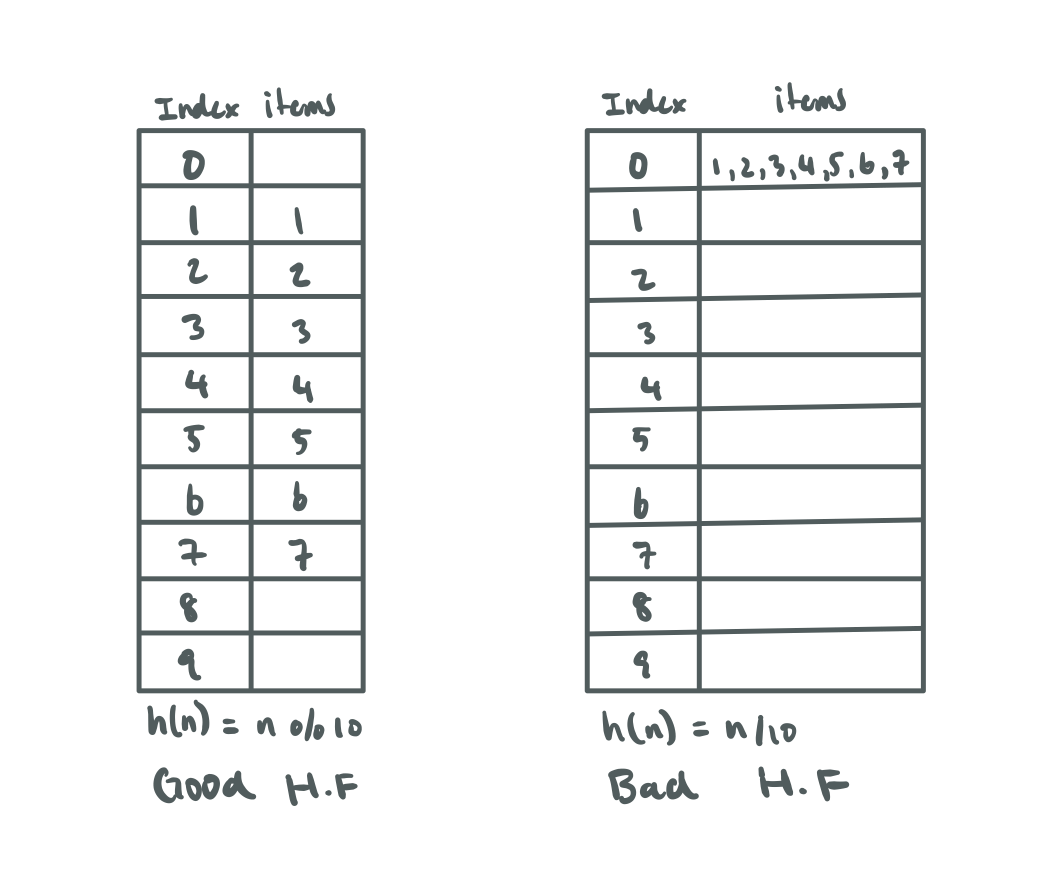
\includegraphics[width=0.95\textwidth]{HashFunction.png}
        \caption{Good vs Bad Hash Functions}
        \label{fig:hashfunc}
    \end{center}
\end{figure}
\textbf{Collisions}
\begin{itemize}
    \item Occurs when two objects map to the same hash value
    \begin{itemize}
        \item Objects $o_1$ and $o_2\rightarrow h(o_1)=h(o_2)$
        \item Unavoidable since $n>m$
    \end{itemize}
    \item Can be dealt with:
    \begin{itemize}
        \item Chaining
        \item Probing/Open addressing
        \item Double hashing
    \end{itemize}
\end{itemize}
%----Chaining----%
\subsubsection{Chaining}
\begin{definition}
    \textit{Chaining}
    \begin{itemize}
        \item Group items with the same hash value (via a hash function) into a bucket (AKA a chain)
        \item e.g. Figure \vref{fig:hashfunc}
        \item \textbf{Time Complexity}:
        \begin{itemize}
            \item \textit{Worst-case}: Hash table becomes a single LL if elements are mapped to one bucket - $O(n)$ search
            \item \textit{Best-case}: Search can become $O(1)$, but is actually $O(n/m)$
            \begin{itemize}
                \item $m$ size of the table, $n$ number of elements to be hashed
            \end{itemize}
        \end{itemize}
    \end{itemize}
\end{definition}
\textbf{Hashable Objects}
\begin{lstlisting}
    public class HashableObject implements Hashable {
        private String key;
        // Other aspects of the object
        public HashableObject(String s) {
            key = new String(s);
        }
        public String key() {
            return key;
        }
    }
\end{lstlisting}
\textbf{3 Hash Functions, each used for different scenarios}
\begin{itemize}
    \item \textit{Hash Function 1}
    \item Fast, but not good for large table sizes
    \begin{lstlisting}
        public class HF1 extends HF {
            public int hash(String s, int size) {
                int hashVal = 0;
                for (int i = 0; i < s.length; i++) {
                    hashVal += s.charAt(i);
                    // Returns int code, e.g. A 65, B 66, etc
                }
                return hashVal % size;
            }
        }
    \end{lstlisting}
    \newpage
    \item \textit{Hash Function 2}
    \item Fast, generally better than HF1, but horrible distributions of values where the first 3 chars are frequent
    \begin{lstlisting}
        public class HF2 extends HF {
            public int hash(String s, int size) {
                int hashVal = 0;
                for (int i = 0; i < s.length; i++) {
                    if (i == 0) { hashVal += s.charAt(0);}
                    else if (i == 1) {hashVal += 27 * s.charAt(1);}
                    else if (i == 2) {hashVal += 729 & s.charAt(2);}
                }
                return hashVal % size;
            }
        }
    \end{lstlisting}
    \item \textit{Hash Function 3}
    \item Fast and has good distribution
    \begin{lstlisting}
        public class HF3 extends HF {
            public int hash(String s, int size) {
                int hashVal = 0;
                for (int i = 0; i < s.length; i++) {
                    hashVal += 37 * hashVal + s.charAt(i);
                }
            hashVal % size;
            if (hashVal < 0) {hashVal += size;}
            return hashVal;
            }
        }
    \end{lstlisting}
\end{itemize}
%----Hash Table implementation with Chaining----%
\textbf{Hash Table implementation with Chaining}
\begin{itemize}
    \item The interface includes clear(), add(), remove(), and contain()
    \begin{lstlisting}
        public class HashTableSC<T extends Hashable> implements HashTableInterface<T> {
            private LinkedList<T>[] hashTable;
            private HashFunction f;

            public HashTableSC(HashFunction f, int m) {
                hashTable = new LinkedList[m];
                this.f = f;
            }
            // Clear 
            public void clear() {
                for (int i = 0; i < hashTable.length; i++) {
                    hashTable[i] = null;
                }
            }
            // Insertion 
            public void add(T item) {
                int i = f.hash(item.key(), hashTable.length);
                if (hashTable[i] == null) {
                    hashTable[i] = new LinkedList<T>();
                }
                hashTable[i].add(item);
            }

            // Deletion
            public void remove(T item) {
                hashTable[f.hash(item.key(), hashTable.length)].remove(item.key());
                // Code before .remove will give you the Chain
            }
            // Search
            public boolean contains(T item) {
                int i = f.hash(item.key(), hashTable.length);
                if (hashTable[i] == null) {return false; }
                else {return hashTable[i].contains(item); }
            }
        }
    \end{lstlisting}
    \item \textbf{Correctness}: follows the correctness of regular LL operations
    \item \textbf{Time Complexity} (with Chaining):
    \begin{itemize}
        \item \textit{Load factor} $\lambda$ of a hash table is the average length of chains $$(n_0+n_1+...+n_{m-1})/m = n/m = \lambda$$
        \item Search analysis: $O(1+\lambda)$, but can be proven $\Theta(1+\lambda)$ 
        \item Insertion analysis: \textbf{Average}: $\Theta(1)$, \textbf{W.C}: $O(n)$
        \item Deletion analysis: \textbf{Average}: $O(1+\lambda)$, \textbf{W.C}: $O(n)$
    \end{itemize}
\end{itemize}
%----Open Addressing----%
\subsubsection{Open Addressing}
\begin{definition}
    \textbf{Open Addressing}
    \begin{itemize}
        \item Method for handling collisions
        \item All elements are stored in the hash table
        \item When \textit{collision} occurs, probe the table until a free (null) entry is found
        \begin{figure}[H]
            \begin{center}
                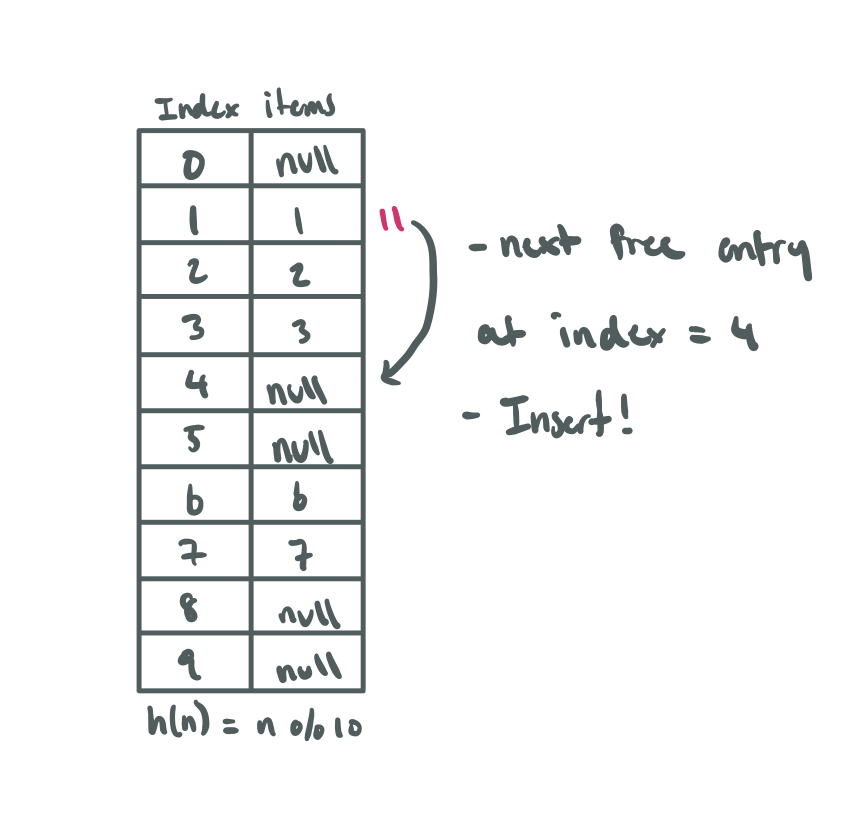
\includegraphics[width=0.6\textwidth]{OpenAddressing.png}
                \caption{Insert 11 in hash table (via hash function)}
            \end{center}
        \end{figure}
        \item \textbf{Linear Probing}
        \begin{itemize}
            \item Prior to inserting 11 at index 4, we had to go through previous indicies to check if they were free
            \item That is $\rightarrow h(k)+0, h(k)+1, h(k)+2, h(k)+3$
            \item Can be represented by: $<h(k),0>,<h(k),1>,<h(k),2>,...$
            \item This is the \textbf{probing sequence}, which gives us a new hashing function $$h'(k)=h(k)+(i \mod 10)$$
            \item This is called \textbf{Linear Probing}
            \begin{itemize}
                \item Variations: Quadratic, double-hashing, etc.
            \end{itemize} 
        \end{itemize}
    \end{itemize}
\end{definition}
%----Algorithms for Linear Probing----%
\textbf{Algorithms for Linear Probing}
\begin{algorithm}
    \caption{Inserting a key \textit{k}}
    $i = 0$\;
    \While{$i<m$}
        {$j=h(k,i)$\;
        \uIf{($T[j]==null$ or $T[j]==Deleted$)}
            {$T[j]=k$\;
            return j\;}
        $i=i+1$\;}
    Throw a TableFullException\;
\end{algorithm}
\textbf{Example of Insertion}
\begin{figure}[H]
    \begin{center}
        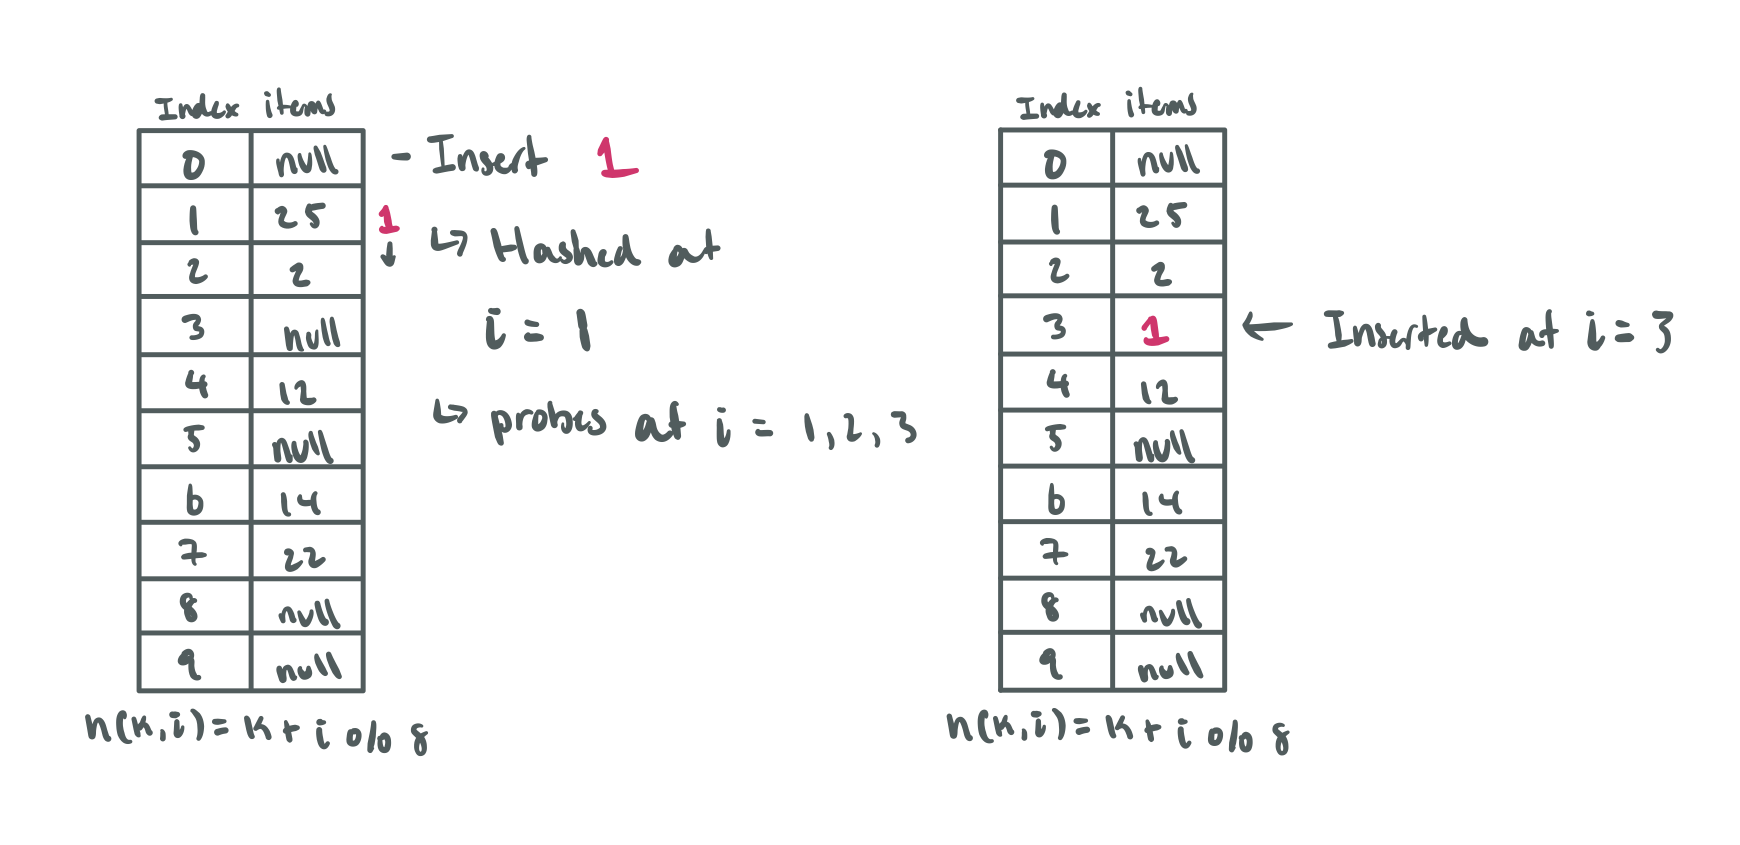
\includegraphics[width=\textwidth]{OAInsert.png}
        \caption{Insert 1}
    \end{center}   
\end{figure}
\begin{algorithm}
    \caption{Searching a key \textit{k}}
    $i = 0$\;
    \While{$i<m$}
        {$j=h(k,i)$\;
        \uIf{($T[j]==k$)}
            {return j\;}
        \uElseIf{$T[j]==null$}
            {Throw a NoSuchElementException\;}
        $i=i+1$\;}
\end{algorithm}
\newpage
\textbf{Example of Searching}
\begin{figure}[H]
    \begin{center}
        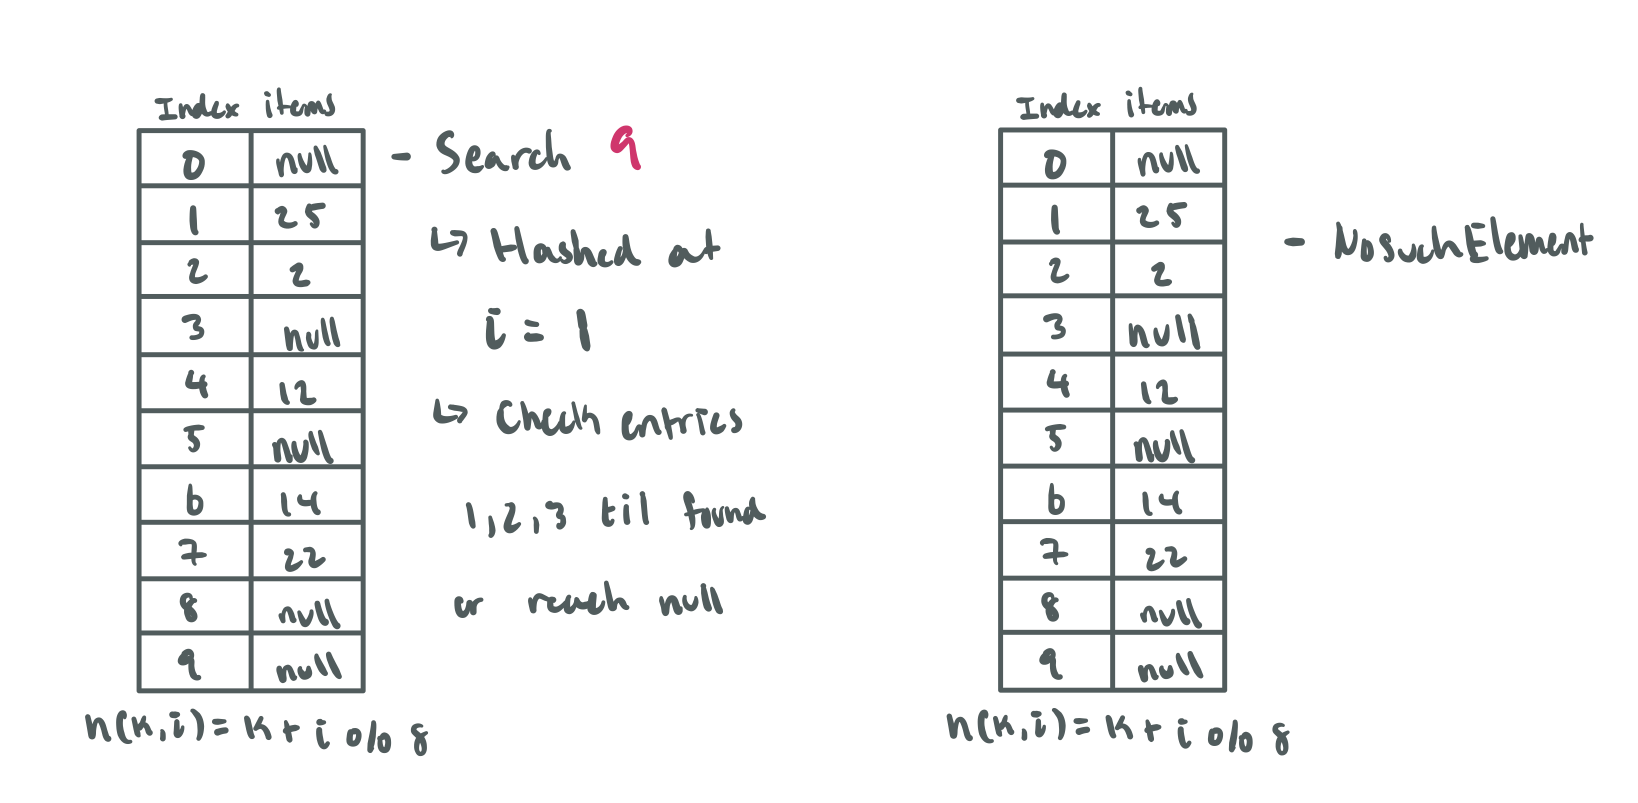
\includegraphics[width=\textwidth]{OASearch.png}
        \caption{Search 9}
    \end{center}   
\end{figure}

\begin{algorithm}
    \caption{Deleting a key \textit{k}}
    $i = 0$\;
    \While{$i<m$}
        {$j=h(k,i)$\;
        \uIf{($T[j]==k$)}
            {$T[j]==deleted$\;
            return\;}
        \uElseIf{($T[j]==null$)}
            {Throw a NoSuchElementException\;}
        $i=i+1$\;}
    Throw a NoSuchElementException\;
\end{algorithm}
\newpage
\textbf{Example of Deletion}
\begin{figure}[H]
    \begin{center}
        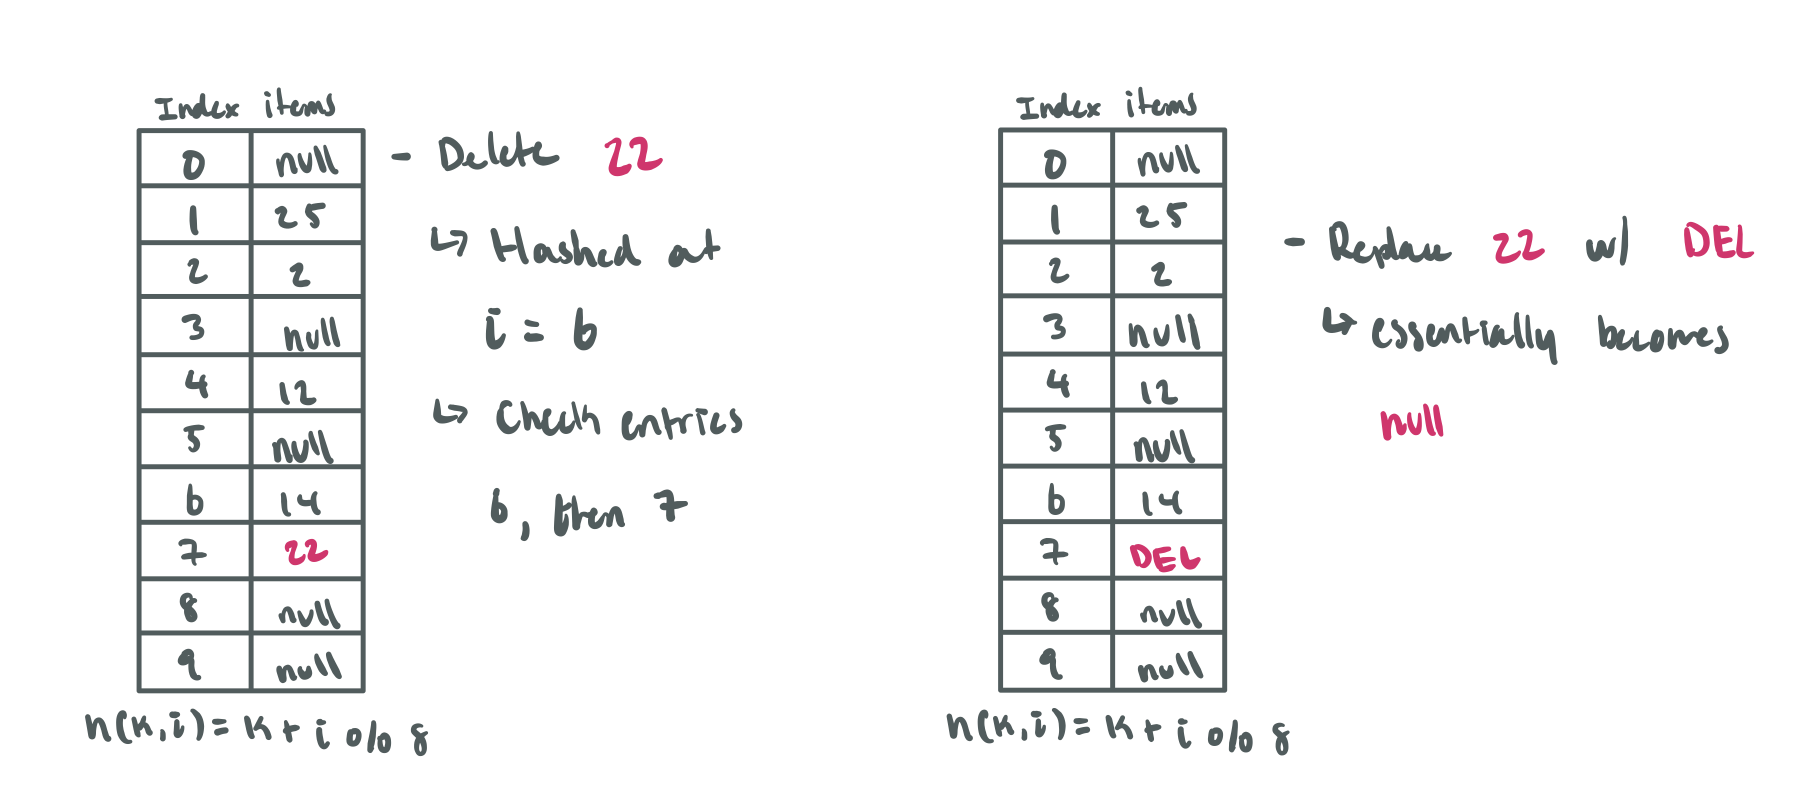
\includegraphics[width=\textwidth]{OADelete.png}
        \caption{Delete 22}
    \end{center}   
\end{figure}
\newpage
%-----------------------------------------------------------------------------------%
%--Graphs--%
\subsection{Graphs}
\textbf{Relations}
\begin{itemize}
    \item $S = \{1, 2, 3\}$
    \item $S \times S = \{(1, 1), (1, 2), (1, 3), (2, 1), (2, 2), (2, 3), (3, 1), (3, 2), (3, 3)\}$
    \item $(S, <) = \{(1, 2), (1, 3), (2, 3)\}$
    \item $(S, \geq) = \{(1, 1), (2, 1), (2, 2), (3, 1), (3, 2), (3, 3)\}$
\end{itemize}
\textbf{Connected}
\begin{itemize}
    \item An undirected Graph, G, is connected if there exists a path between each pair of vertices in G
    \item Node E does not have a directed path outward
    \begin{figure}[H]
        \begin{center}
            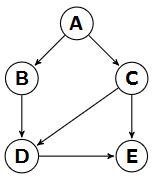
\includegraphics[width=0.2\textwidth]{Graph1.png}
        \end{center}
    \end{figure}
\end{itemize}
\textbf{Weakly Connected}
\begin{itemize}
    \item G is weakly connected if the undirected underlying graph obtained by replacing every directed edge by
    an undirected edge is connected
    \begin{figure}[H]
        \begin{center}
            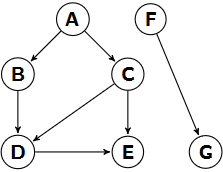
\includegraphics[width=0.2\textwidth]{Graph2.png}
        \end{center}
    \end{figure}
\end{itemize}
\textbf{Strongly Connected}
\begin{itemize}
    \item G is strongly connected if there is a directed path between each pair of vertices in G
    \item There is a directed path from every node to another node in G
    \begin{figure}[H]
        \begin{center}
            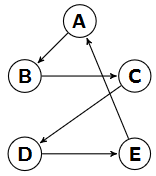
\includegraphics[width=0.2\textwidth]{Graph3.png}
        \end{center}
    \end{figure}
\end{itemize}
\textbf{Directed Free Tree}
\begin{itemize}
    \item Is a connected acyclic directed graph
    \item A tree is a free tree with:
    \begin{itemize}
        \item Exactly one vertex has no edges going outward (the root)
        \item An ordering of the children (adjacent-from) of each vertex
    \end{itemize}
    \begin{figure}[H]
        \begin{center}
            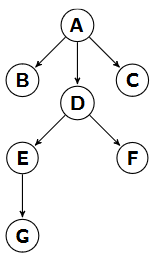
\includegraphics[width=0.2\textwidth]{Graph4.png}
        \end{center}
    \end{figure}
\end{itemize}
\begin{figure}[H]
    \begin{center}
        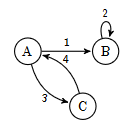
\includegraphics[width=0.2\textwidth]{Graph5.png}
    \end{center}
\end{figure}
\textbf{Adjacency Matrix}
\begin{itemize}
    \item Represented as an $n \times n$ array
    \item Good for small graphs
    \item Can result in sparse graphs at large scales
    \item If the graph is undirected, then the adjacency matrix will be mirrored over $y=x$
    \begin{center}
        \begin{tabular}{|c|c|c|c|}
            \hline
             & \textbf{A} & \textbf{B} & \textbf{C} \\
            \hline
            \textbf{A} & 0 & 1 & 3 \\
            \hline
            \textbf{B} & 0 & 2 & 0 \\
            \hline
            \textbf{C} & 4 & 0 & 0 \\
            \hline
        \end{tabular}
    \end{center}
\end{itemize}
\textbf{Adjacency List}
\begin{itemize}
    \item Represented as an array (or LL) where each element is a pointer to the head of a different LL
    \item Solves the problem for sparse graphs 
    \item Better for larger graphs 
    \item \textbf{Note}: AL[0] corresponds to \textbf{A}, AL[1] to \textbf{B}, AL[2] to \textbf{C} $$AL[0]\rightarrow [(B,1)\rightarrow (C,3)]$$ 
    $$AL[1]\rightarrow [(B,2)]$$ $$AL[2]\rightarrow [(A,4)]$$ 
\end{itemize}
\newpage
%-----------------------------------------------------------------------------------%
%--Dijkstra's Algorithm--%
\subsection{Dijkstra's Algorithm}
%----Algorithm----%
\subsubsection{Algorithm}
\begin{lstlisting}
    int[] Dijkstra(Graph g, int start) {
        Set<Integer> seen = {start};
        for (each v in g.vertices) {
            distance[v] = g.adjacencyMatrix[start][v]; // Distance array of initial cost of paths 
        }                                                   // from start to all other vertices
        repeat(n - 1 times) {
            Choose a vertex w in vertices not seen where distance[w] is the minimum currently;
            add w to seen; 
            for (each v not seen) {
                distance[v] = min(distance[v], distance[w] + g.adjacencyMatrix[w][v]);
            }   // Going from start to v could be cheaper through w
        }
        return distance;
    }
\end{lstlisting}
%----Example----%
Consider the following:
\begin{figure}[H]
    \begin{center}
        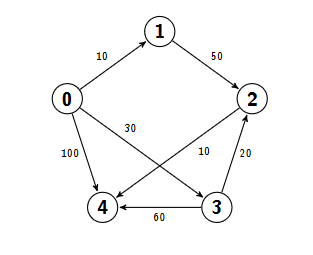
\includegraphics[width=0.4\textwidth]{DijkstraExample.png}
        \caption{Example of a Directed Weighted Graph}
    \end{center}
\end{figure}
\textbf{Start of 1st Iteration}
\begin{itemize}
    \item w = 1 since distances[w] is the minimum value the is not marked as seen (Node 0 is marked as seen initially)
    \item $seen = \{0\}$
    \item $distance = \{0,10,\infty,30,100\}$
    \begin{center}
        \begin{tabular}{|c|c|c|c|c|c|}
            \hline
            & \textbf{0} & \textbf{1} & \textbf{2} & \textbf{3} & \textbf{4} \\
            \hline
            \textbf{0} & 0 & 10 & $\infty$ & 30 & 100 \\
            \hline
        \end{tabular}
    \end{center}
    \item $path = \{0,0,0,0,0\}$
    \begin{center}
        \begin{tabular}{|c|c|c|c|c|}
            \hline
            0 & 0 & 0 & 0 & 0 \\
            \hline
        \end{tabular}
    \end{center}
    \item Values at each index of path represent the current node we are at
    \item Each index represents the next node in the shortest path that we can get to from the current node
\end{itemize}
\textbf{End of 1st Iteration}
\begin{itemize}
    \item w = 1 (still)
    \item $seen = \{0,1\}$
    \item $distance = \{0,10,60,30,100\}$ 
    \begin{center}
        \begin{tabular}{|c|c|c|c|c|c|}
            \hline
            & \textbf{0} & \textbf{1} & \textbf{2} & \textbf{3} & \textbf{4} \\
            \hline
            \textbf{0} & 0 & 10 & $\infty$ & 30 & 100 \\
            \hline
            \textbf{1} & 0 & 10 & 60 & 30 & 100 \\
            \hline
        \end{tabular}
    \end{center}
    \item $path = \{0,0,1,0,0\}$
    \item Now that we have seen node 1, we know it is possible to get to node 2 by traversing to 1 and then 2 which
    has a weight of 10 + 50 = 60
    \item Since node 1 only points to 2, the rest of the distances do not change
    \begin{center}
        \begin{tabular}{|c|c|c|c|c|}
            \hline
            0 & 0 & 1 & 0 & 0 \\
            \hline
        \end{tabular}
    \end{center}
    \item It is possible to get to all nodes through 0 except node 2 which is from 0 → 1 → 2 currently
    \item Currently, the shortest path to node 2 is through node 1
\end{itemize}
\textbf{Start of 2nd Iteration}
\begin{itemize}
    \item w = 3 since distances[w] is the minimum value of the nodes not seen after the first iteration (30 is the smallest
    of $\{60, 30, 100\}$)
    \item $seen = \{0, 1\}$ (still)
    \item $distances = \{0, 10, 60, 30, 100\}$ (still)
    \item $path = \{0, 0, 1, 0, 0\}$ (still)
\end{itemize}
\textbf{End of 2nd Iteration}
\begin{itemize}
    \item w = 3 (still)
    \item $seen = \{0, 1, 3\}$
    \item $distances = \{0, 10, 50, 30, 90\}$
    \begin{center}
        \begin{tabular}{|c|c|c|c|c|c|}
            \hline
            & \textbf{0} & \textbf{1} & \textbf{2} & \textbf{3} & \textbf{4} \\
            \hline
            \textbf{0} & 0 & 10 & $\infty$ & 30 & 100 \\
            \hline
            \textbf{1} & 0 & 10 & 60 & 30 & 100 \\
            \hline
            \textbf{2} & 0 & 10 & 50 & 30 & 90 \\
            \hline
        \end{tabular}
    \end{center}
    \item Shortest path to node 2 is now through node 3 which has a cost of 30 + 20 = 50
    \item Shortest path to node 3 is unchanged
    \item Shortest path to node 4 is updated since 90 < 100 and this is cost is calculated by 30 + 60
    \item $path = \{0, 0, 3, 0, 3\}$
    \begin{center}
        \begin{tabular}{|c|c|c|c|c|}
            \hline
            0 & 0 & 3 & 0 & 3 \\
            \hline
        \end{tabular}
    \end{center} 
    \item Shortest path to node 2 is changed from 0 → 1 → 2 to 0 → 3 → 2
    \item Shortest path to node 4 is changed from 0 → 4 to 0 → 3 → 4
\end{itemize}
\textbf{Start of 3rd Iteration}
\begin{itemize}
    \item w = 2 since distances[w] is the minimum cost of the nodes we have not seen. That is, distances[2] = 50 is the
    minimum of $\{50, 90\}$
    \item $seen = \{0, 1, 3\}$ (still)
    \item $distances = \{0, 10, 50, 30, 90\}$ (still)
    \item $path = \{0, 0, 3, 0, 3\}$ (still)
\end{itemize}
\textbf{End of 3rd Iteration}
\begin{itemize}
    \item w = 2 (still)
    \item $seen = \{0, 1, 3, 2\}$
    \item $distances = \{0, 10, 50, 30, 60\}$
    \begin{center}
        \begin{tabular}{|c|c|c|c|c|c|}
            \hline
            & \textbf{0} & \textbf{1} & \textbf{2} & \textbf{3} & \textbf{4} \\
            \hline
            \textbf{0} & 0 & 10 & $\infty$ & 30 & 100 \\
            \hline
            \textbf{1} & 0 & 10 & 60 & 30 & 100 \\
            \hline
            \textbf{2} & 0 & 10 & 50 & 30 & 90 \\
            \hline
            \textbf{3} & 0 & 10 & 50 & 30 & 60 \\
            \hline
        \end{tabular}
    \end{center}
    \item The only node we can to from node 2 is 4 so all weights except 4 are unchanged
    \item The cost to node 4 is updated as the cost to node 2 plus the cost to get from 2 → 4 which is 50 + 10 = 60 and
    since 60 < 90, it is updated
    \item $path = \{0, 0, 3, 0, 2\}$
    \begin{center}
        \begin{tabular}{|c|c|c|c|c|}
            \hline
            0 & 0 & 3 & 0 & 2 \\
            \hline
        \end{tabular}
    \end{center} 
    \item The paths array is also updated for shortest path to node 4 is changed to 0 → 3 → 2 → 4
\end{itemize}
\textbf{Start of 4th Iteration}
\begin{itemize}
    \item w = 4 since it is the only node that has not yet been seen so it is certainly a minimum of what is still unseen
    \item $seen = \{0, 1, 3, 2\}$ (still)
    \item $distances = \{0, 10, 50, 30, 60\}$ (still)
    \item $path = \{0, 0, 3, 0, 2\}$ (still)
    \item However, node 4 does not have any edges directed outwards thus there is nothing more that can be done
\end{itemize}
\textbf{End of 4th Iteration}
\begin{itemize}
    \item $seen = \{0, 1, 3, 2, 4\}$
    \item Everything else the same
\end{itemize}
\textbf{Generating the Shortest Path}
\begin{itemize}
    \item Let our starting point be some node, start
    \item Let our destination point be some node, dest, then set $current = dest$
    \item Now, while current $\neq$ start then current = paths[current] to get the next node in the shortest path working
    our way backwards from the destination to the start
    \item \textbf{Ex}:
    \begin{itemize}
        \item Let start = 0, dest = 4
        \item Lets record each node we see in a dynamic array, $arr = \{\}$
        \item \textbf{Iteration 1}
        \begin{itemize}
            \item current = 4
            \item $current \neq 0$
            \item Then, current = paths[4] = 2, $arr = \{4\}$
        \end{itemize}
        \item \textbf{Iteration 2}
         \begin{itemize}
            \item current = 2
            \item $current \neq 0$
            \item Then, current = paths[2] = 3, $arr = \{2, 4\}$
        \end{itemize}
        \item \textbf{Iteration 3}
        \begin{itemize}
            \item current = 3
            \item $current \neq 0$
            \item Then, current = paths[3] = 0, $arr = \{3, 2, 4\}$
        \end{itemize}
        \item \textbf{Iteration 4}
        \begin{itemize}
            \item current = 0
            \item $current = 0$ is true
            \item Add it: $arr = \{0, 3, 2, 4\}$
        \end{itemize}
        \item Now, the shortest path from node 0 to node 4 has been obtained
    \end{itemize}
\end{itemize}
%----Correctness----$
\subsubsection{Correctness}
\begin{definition}
    \textit{Loop Invariant}
    \begin{itemize}
        \item \textit{\textbf{Initialization}}
        \begin{itemize}
            \item Before the first iteration, $S_0$ only contains start and all special paths that exist from start to other vertices
            that have a single edge
            \item All existing such special paths are the shortest and $D_0[v]$ contains their cost
            \item Otherwise, $D_0[v] = \infty$
        \end{itemize}
        \item \textit{\textbf{Maintenance}}
        \begin{itemize}
            \item Assume $D_{i-1}[v]$ contains the cost of the shortest special path from start to v
            \item We show that $D_i[v]$ contains the cost of the shortest special path from start to v
            \item In iteration i, we add w to Si where $D_i[w]$ is the minimum
            \item For a vertex v, $D_i[v]$ will be updated if it is shorter to go from start to v through w
        \end{itemize}
        \item \textit{\textbf{Termination}}
        \begin{itemize}
            \item The repeat loop will iterate n - 1 times
            \item Hence, $S_{n-1} = G$. vertices (All vertices have been seen)
            \item After this last iteration, $D_{n-1}[v]$ is the cost of the shortest special path from start to v if such a path exists
            \item If there is not path from start to v, then $D[v] = \infty$
        \end{itemize}
    \end{itemize}
\end{definition}
\newpage
%-----------------------------------------------------------------------------------%
%Sorting Algorithms%
\section{Sorting Algorithms}
%--Bubble Sort--%
\subsection{Bubble Sort}
%----Algorithm----%
\subsubsection{Algorithm}
\begin{lstlisting}
    // Bubble Sort in Sorting
    public void sort() {
        for (i = 0; i < size; i++) {
            for (j = size - 1; j > i; j--) {
                if (list[j].compareTo(list[j-1]) < 0) {
                    T tmp = list[j];
                    list[j] = list[j-1];
                    list[j-1] = tmp;
                }
            }
        }
    }
    // Bubble Sort in BoundedList
    public static void sort(BoundedList list) {
        for (i = 0; i < list.size(); i++) {
            for (j = list.size() - 1; j > i; j--) {
                if (list.getItem(j).compareTo(list.getItem(j-1)) < 0) {
                    list.swap(j, j-1);
                }
            }
        }
    }
    // Main algorithm
    Bubble-Sort(L = list of items, n = size) {
        for (i = 0; i < n; i++) {
            for (j = n - 1; j > i; j--) {
                if (L[j].key < L[j-1].key) {
                    swap(L[j], L[j-1]);
                }
            }
        }
    }
    // Where swap() is...
    swap(item n1, item n2) {
        tmp = n1;
        n1 = n2;
        n2 = tmp;
    }
\end{lstlisting}
\newpage
\textbf{Example}:
\begin{figure}[H]
    \begin{center}
        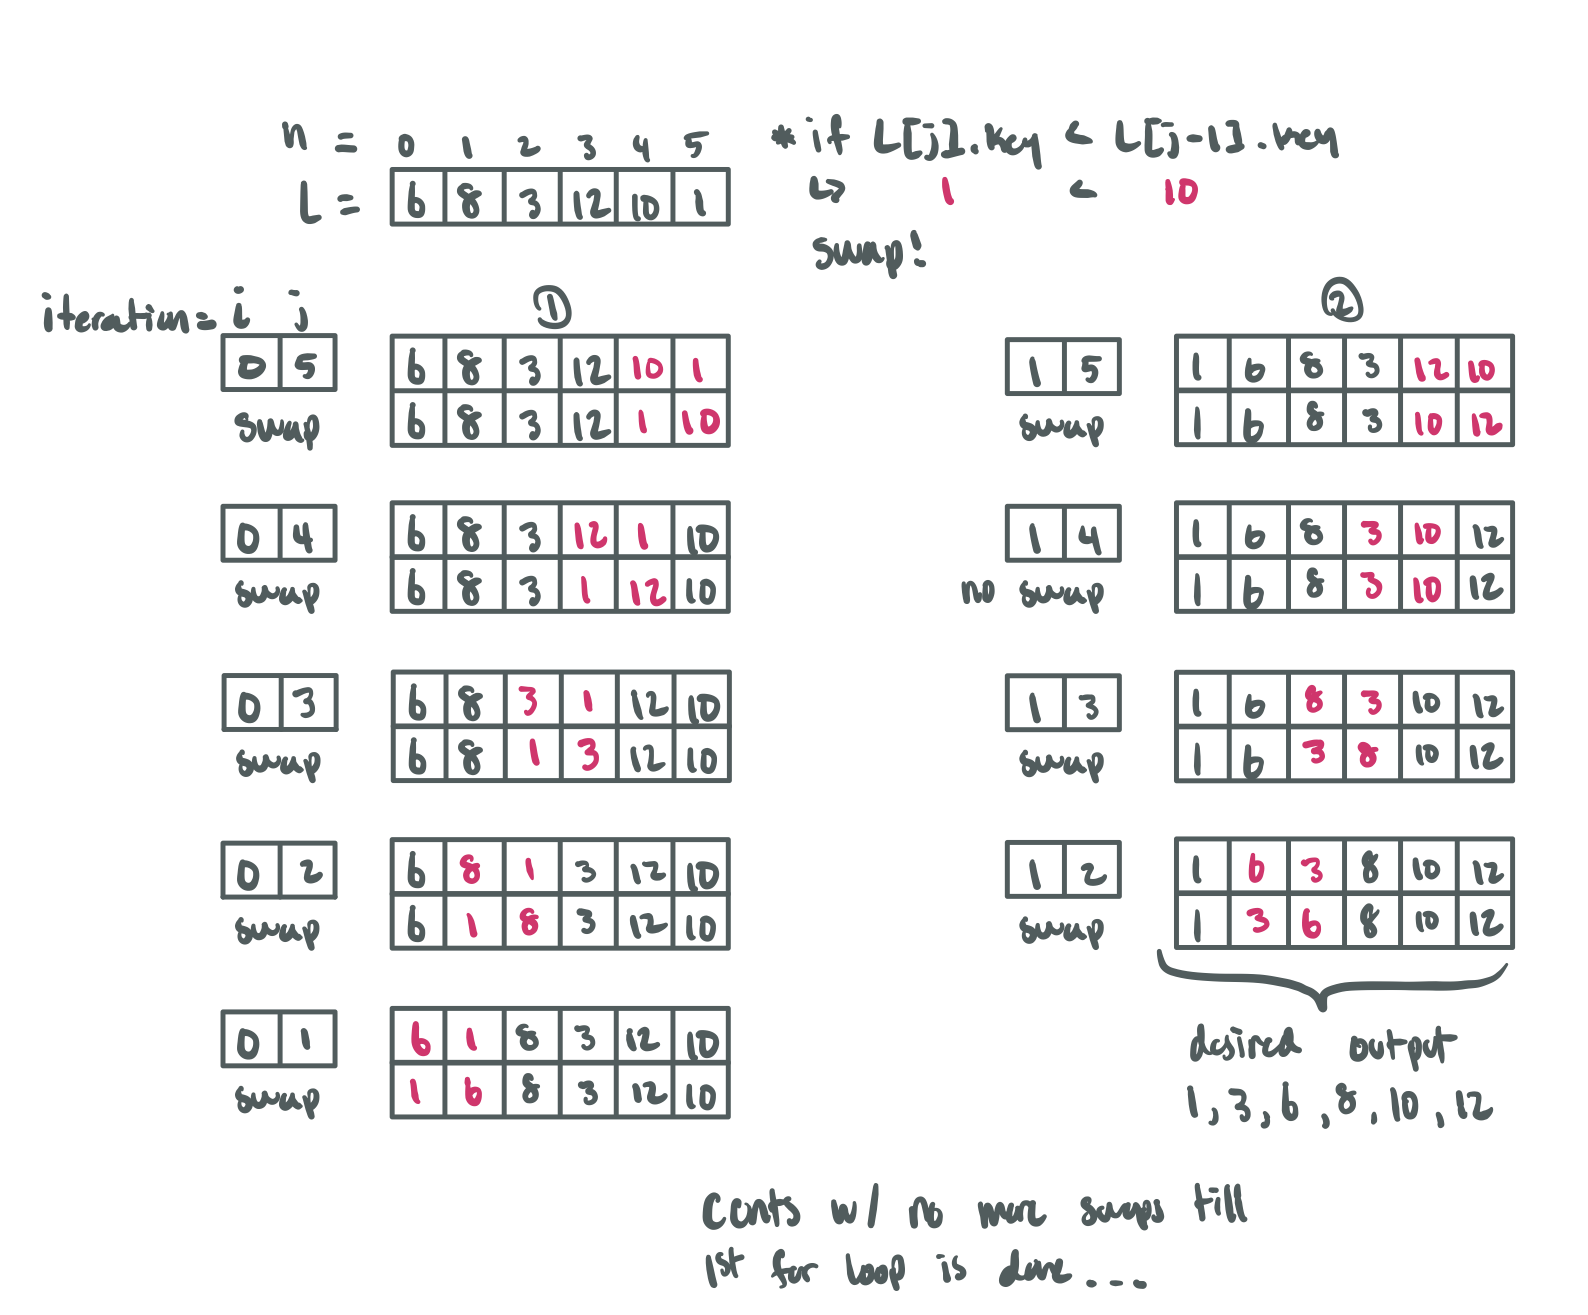
\includegraphics[width=\textwidth]{BubbleSort.png}
        \caption{Bubble sort following the main algorithm}
    \end{center}
\end{figure}
%----Time Complexity----%
\subsubsection{Time Complexity}
\begin{definition}
    \textit{Time Complexity}
    \begin{itemize}
        \item \textbf{swap()}: $\Theta(1)$
        \item \textbf{j-loop}: executed $n-i-1$ times
        \item \textbf{i-loop}: executed $n$ times
        \item \textbf{Bubble-Sort}: $\Sigma^{n-1}_{i=0}n-i-1$ $$\Sigma^{n-1}_{i=0}n-i-1=(n-1)+(n-2)+...+1+0=\frac{n^2-n}{2}$$
        \item \textbf{Hence}, Bubble-Sort is quadratic, $\Theta(n^2)$
    \end{itemize}
\end{definition}
\newpage
%----Correctness----%
\subsubsection{Correctness}
\begin{definition}
    \textit{Loop Invariant}
    \begin{itemize}
        \item \textbf{Inner Loop}
        \begin{itemize}
            \item \textit{Initialization}:
            \begin{itemize}
                \item Initially, $j=n-1$ and $L[n-1...n-1]$ is a singleton
                \begin{itemize}
                    \item LI is vacuously satsified
                \end{itemize}
            \end{itemize}
            \item \textit{Maintenance}:
            \begin{itemize}
                \item Assume LI is correct before iteration $j=k$
                \item That is, $L[k]$ is the min in $L[k...n-1]$
                \item In iteration $j=k$
                \begin{itemize}
                    \item If $L[k].key<L[k-1].key$, then swap($L[k],L[k-1]$), making $L[k-1]$ the new min in $L[k-1...n-1]$
                    \item Else, item being considered $L[k-1].key \leq L[k].key$, meaning that $L[k-1]$ is the min in $L[k-1...n-1]$
                    \item Hence, before the next iteration $j=k-1$, $L[k-1]$ is the min in $L[k-1...n-1]$
                \end{itemize}
            \end{itemize}
            \item \textit{Termination}:
            \begin{itemize}
                \item Last iteration of the loop is when $j=i-1$
                \item Hence, by LI, $L[i]$ is the min item in $L[i...n-1]$
            \end{itemize}
        \end{itemize}
        \item \textbf{Outer Loop}
        \begin{itemize}
            \item \textit{Initialization}:
            \begin{itemize}
                \item Before the first iteration, $i=0$ and $L[0...i-1]$ is empty and LI is vacuously true
            \end{itemize}
            \item \textit{Maintenance}:
            \begin{itemize}
                \item Assume LI is correct before iteration $i=k$
                \item Hence, $L[0...k-1]$ is a sorted list of the smallest \textit{k} items in L
                \item In iteration $i=k$, by the LI of the \textbf{inner loop}:
                \begin{itemize}
                    \item $L[k]$ is the min item in $L[k...n-1]$
                \end{itemize}
                \item Since $L[0...k-1]$ has the smallest \textit{k} items of L in sorted order,
                \item $L[0...k]$ will have the smallest $k+1$ items in L in sorted order
            \end{itemize}
            \item \textit{Termination}:
            \begin{itemize}
                \item Last iteration of the loop is when $i=n-1$
                \item Hence, when the loop terminates, $L[0...n-2]$ is a sorted permutation of the smallest $n-1$ elements in L
                \item Since $L[n-1]$ was considered the last iteration and compared with $L[n-2]$, it must be the case that $L[n-1]$ is the largest 
                item in L
                \item Therefore, when the loop terminates, $L[0...n-1]$ is a sorted permutation of the original elements in L
            \end{itemize}
        \end{itemize}
    \end{itemize}
\end{definition}
\newpage
%-----------------------------------------------------------------------------------%
%--Selection Sort--%
\subsection{Selection Sort}
%----Algorithm----%
\subsubsection{Algorithm}
\begin{lstlisting}
    // Selection sort in Sorting
    public static void selectionSort(BoundedList list) {
        for (int i = 0; i < list.size(); i++) {
            int minIndex = list.getMinIndex(i, list.size()-1);
            list.swap(i, minIndex);
        }
    }
    // Main algorithm
    Selection-Sort(L = list of items, n = size) {
        for (i = 0; i < n; i++) {
            min = Find-Min(L[i...n-1]);
            swap(L[i], min);
        }
    }
    // Find minimum
    Find-Min(L = list of items, n = size) { // Must be non-empty
        currMin = L[0];
        for (i = 1; i < n; i++) {
            if (L[i] < currMin) {
                currMin = L[i];
            }
        }
        return currMin;
    }
\end{lstlisting}
\textbf{Example}:
\begin{figure}[H]
    \begin{center}
        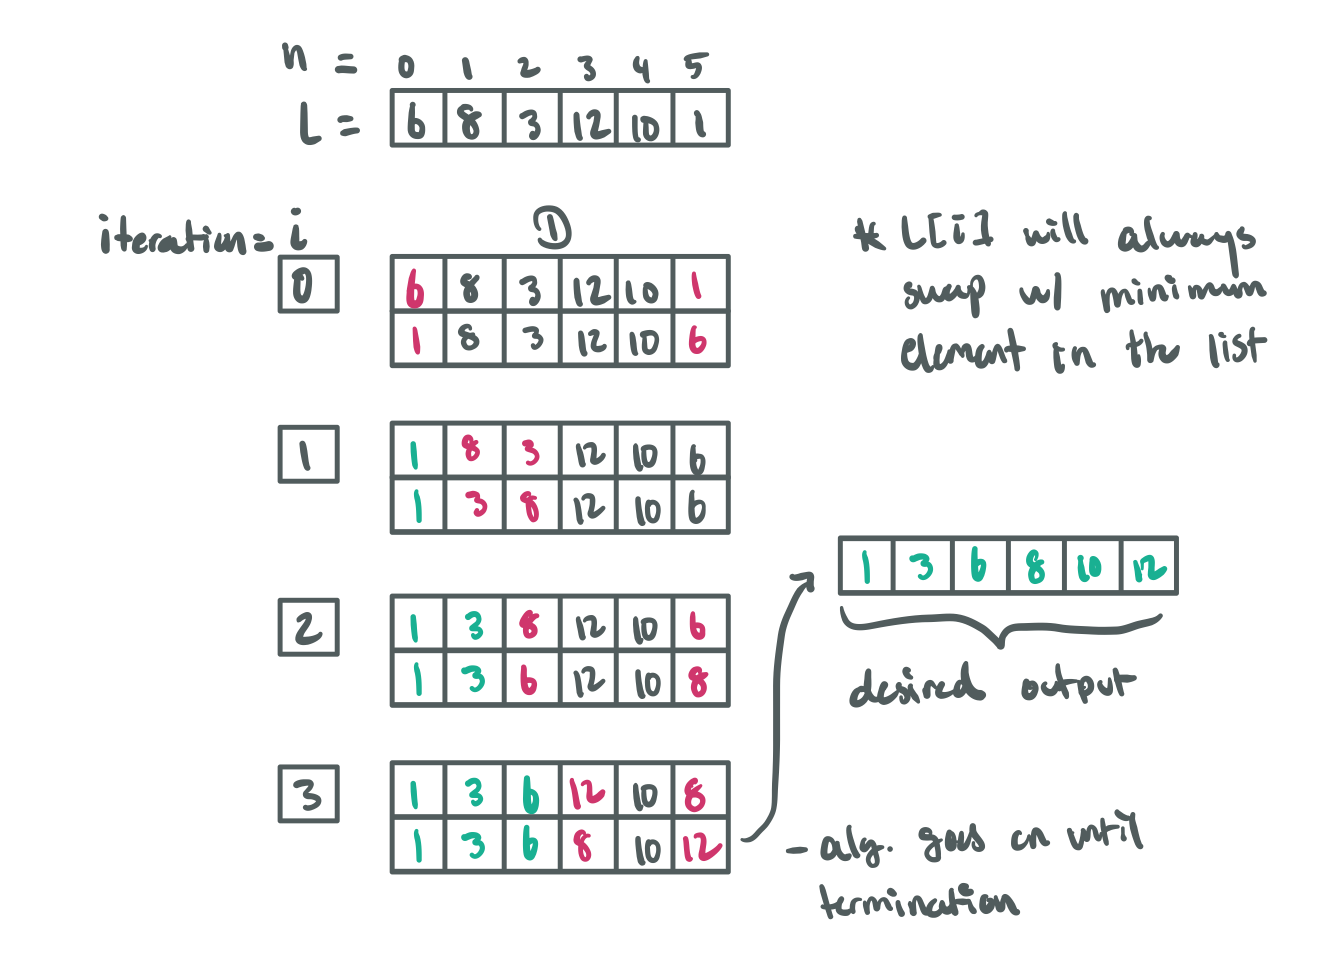
\includegraphics[width=0.7\textwidth]{SelectionSort.png}
        \caption{Selection sort following main algorithm}
    \end{center}
\end{figure}
%----Time Complexity----%
\subsubsection{Time Complexity}
\begin{definition}
    \textit{Time Complexity}
    \begin{itemize}
        \item \textbf{loop}: executed $n-1$ times
        \item \textbf{Find-Min()}: $\Theta(n)$ on all cases
        \begin{itemize}
            \item List is reduced by 1 after every iteration
            \item 1st: $|L|=n$
            \item 2nd: $|L|=n-1$
            \item ith: $|L|=n-i-1$
        \end{itemize}
        \item \textbf{Selection-Sort}: $\Sigma^{n-1}_{i=1}n-i-1$ $$\Sigma^{n-1}_{i=1}n-i-1=(n-2)+...+1=\frac{n^2-2n+2}{2}$$
        \item \textbf{Hence}, Selection-Sort is quadratic, $\Theta(n^2)$
    \end{itemize}
\end{definition}
%----Correctness----%
\subsubsection{Correctness}
\begin{definition}
    \textit{Loop Invariant}
    \begin{itemize}
        \item \textbf{Find-Min}
        \begin{itemize}
            \item \textit{\textbf{Initialization}}
            \begin{itemize}
                \item Before the first iteration, \textit{currMin} is $L[0]$, which is the minimum item in the singleton $L[0...0]$
            \end{itemize}
            \item \textit{\textbf{Maintenance}}
            \begin{itemize}
                \item Assume LI is correct before iteration $i=k$
                \item Hence, \textit{currMin} is the min item in $L[0...k-1]$
                \item In iteration $i=k$
                \begin{itemize}
                    \item If $L[k]<currMin$, then $L[k]$ is the min in $L[0...k]$ and \textit{currMin} is updated accordingly
                    \item Else, $L[k]\geq currMin$, \textit{currMin} is still the min item in $L[0...k]$
                \end{itemize}
                \item Hence, LI is also correct after iteration $i=k$
            \end{itemize}
            \item \textit{\textbf{Termination}}
            \begin{itemize}
                \item Last iteration of the for loop is $i=n-1$
                \item Thus, when loop terminates, \textit{currMin} is the min item in $L[0...n-1]$
            \end{itemize}
        \end{itemize}
        \item \textbf{Selection-Sort}
        \begin{itemize}
            \item \textit{\textbf{Initialization}}
            \begin{itemize}
                \item Before the first iteration, the singleton $L[0...-1]$ is empty, LI being vacuously true
            \end{itemize}
            \item \textit{\textbf{Maintenance}}
            \begin{itemize}
                \item Assume LI to be correct before iteration $i=k$
                \item Hence, $L[0...k-1]$ is a sorting of $S[0...k-1]$
                \begin{itemize}
                    \item In iteration $i=k$, min of $L[0...k-1]$ is swapped with $L[k]$
                    \item Since $L[k]$ was not picked as the min in a previous iteration, it must be the case that each item in $L[0...k-1]$ is not bigger than $L[k]$ 
                \end{itemize}
                \item Hence, $L[0...k]$ is sorted
                \item Since the only change introduced to $L[0...k]$ is swapping existing elements of $S[0...k]$, $L[0...k]$ is a sorting of $S[0...k]$
                \item Therefore, LI holds for the end of iteration $i=k$
            \end{itemize}
            \item \textit{\textbf{Termination}}
            \begin{itemize}
                \item Last iteration of the for loop is $i=n-1$
                \item Min of $L[n-2...n-1]$ is moved up to $L[n-2]$ and now $L[n-1]$ has the largest item in the list
                \item Hence, when the loop terminates, $L[0...n-1]$ will be sorted
            \end{itemize}
        \end{itemize}
    \end{itemize}
\end{definition}
\newpage
%-----------------------------------------------------------------------------------%
%--Insertion Sort--%
\subsection{Insertion Sort}
%----Algorithm----%
\subsubsection{Algorithm}
\begin{lstlisting}
    // Insertion Sort in Sorting
    public static void sort(BoundedList list) {
        for (i = 1; i < list.size(); i++) {
            for (j = i; j > 0; j--) {
                if (list.getItem(j).compareTo(list.getItem(j-1)) < 0) {
                    list.swap(j, j-1);
                }
            }
        }
    }
    // Main algorithm
    Insertion-Sort(L = list of items, n = size) {
        for (i = 1; i < n; i++) {
            for (j = i; j > 0; j--) {
                if (L[j].key < L[j-1].key) {
                    swap(L[j], L[j-1]);
                }
            }
        }
    }
    // Where swap() is...
    swap(item n1, item n2) {
        tmp = n1;
        n1 = n2;
        n2 = tmp;
    }
\end{lstlisting}
\textbf{Example}:
\begin{figure}[H]
    \begin{center}
        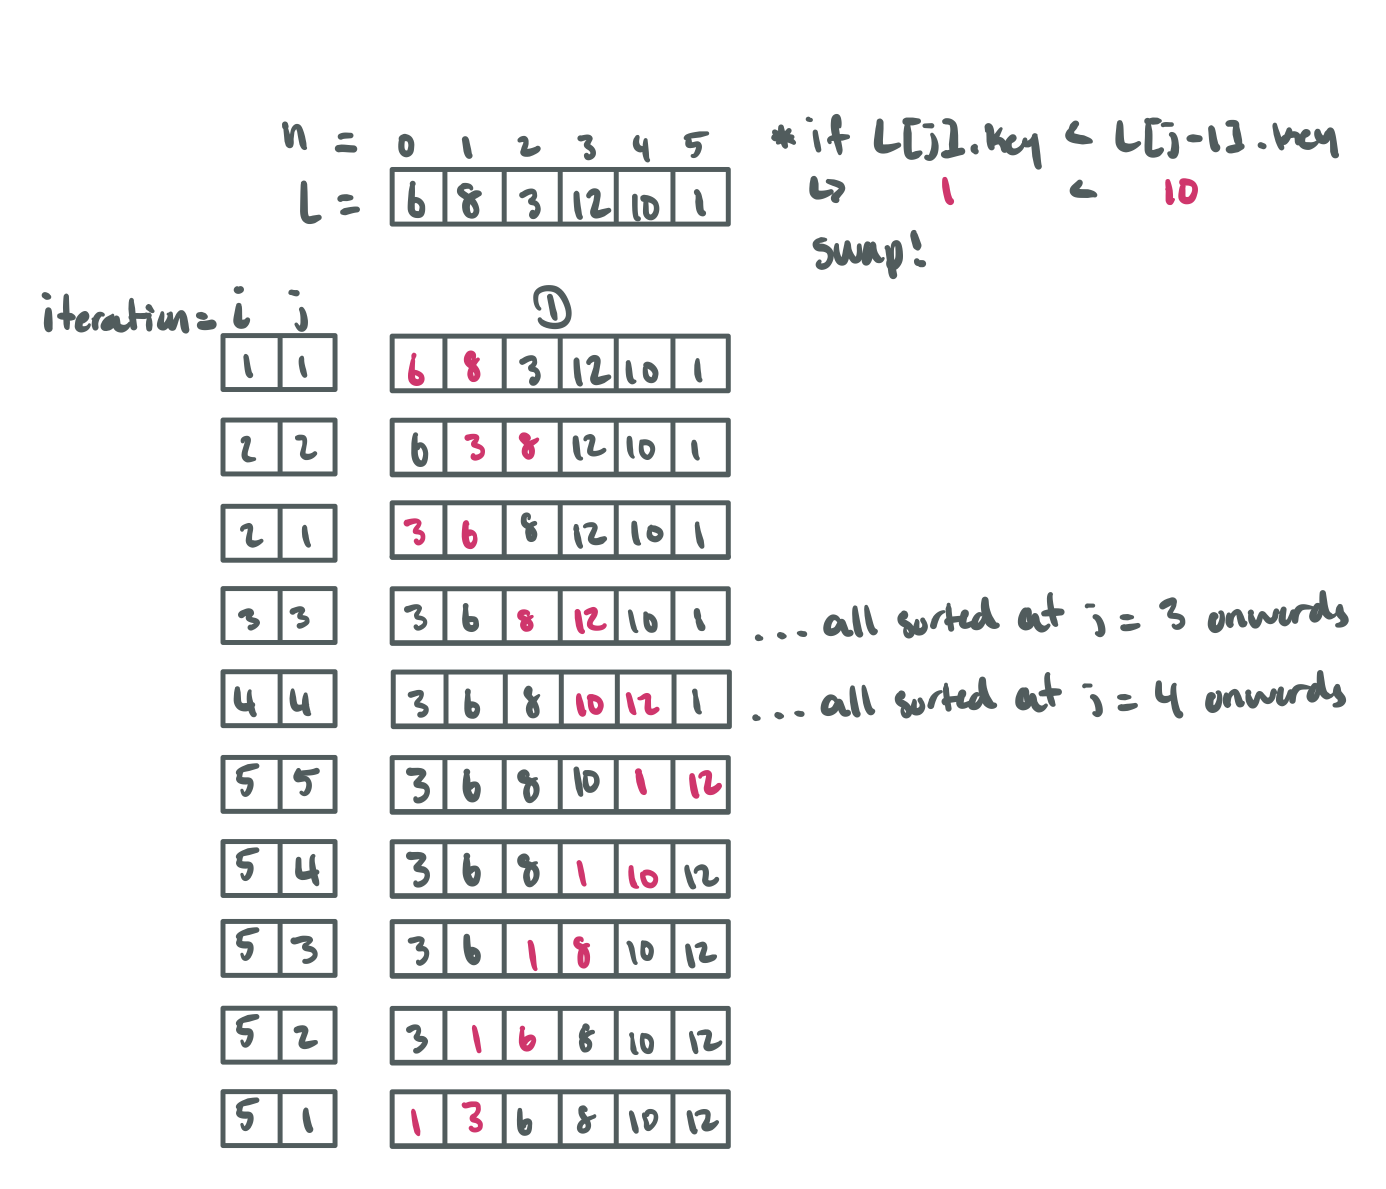
\includegraphics[width=0.65\textwidth]{InsertionSort.png}
        \caption{Insertion sort following the main algorithm}
    \end{center}
\end{figure}
%----Time Complexity----%
\subsubsection{Time Complexity}
\begin{definition}
    \textit{Time Complexity}
    \begin{itemize}
        \item \textbf{swap()}: $\Theta(1)$
        \item \textbf{j-loop}: executed $i$ times
        \item \textbf{i-loop}: executed $n-1$ times, $\Theta(n)$
        \item \textbf{Insertion-Sort}: $\Sigma^{n-1}_{i=1}n-i-1$ $$\Sigma^{n-1}_{i=1}n-i-1=(n-1)+(n-2)+...+1+0=\frac{n^2-n}{2}$$
        \item \textbf{Hence}, Insertion-Sort is quadratic, $\Theta(n^2)$
    \end{itemize}
\end{definition}
%----Correctness----%
\subsubsection{Correctness}
\begin{definition}
    \textit{Loop Invariant}
    \begin{itemize}
        \item \textbf{Inner Loop}
        \begin{itemize}
            \item \textit{\textbf{Initialization}}:
            \begin{itemize}
                \item Initially, $j=i=1$, $L[0...0]$ is a sorted permutation of $S[0]$
                \begin{itemize}
                    \item LI is vacuously satsified
                \end{itemize}
            \end{itemize}
            \item \textit{\textbf{Maintenance}}:
            \begin{itemize}
                \item Assume LI is correct before iteration $j=k$
                \item Hence, $L[k-1...i-1]$ is a sorted permutation of $S[k-1...i-1]$
                \item We show LI still holds at the end of this iteration before $j=k-1$
                \begin{itemize}
                    \item Loop compares $L[k-1],L[k-2]$
                    \item If $L[k-2].key<L[k-1].key$, swap($L[k-2].key, L[k-1].key$)
                    \item Now, $L[k-2...i-1]$ is also a sorted permutation of $S[k-2...i-1]$
                    \item Else, $L[k-2].key$ is larger than $L[k-1].key$, loop does nothing and $L[k-2...i-1]$ is still a sorted
                    permutation of $S[k-2...i-1]$
                \end{itemize}
                \item In both cases, the loop makes sure $L[k-2...i-1]$ has the same items as $S[k-2...i-1]$
                \item Hence, LI still holds at the end of the iteration
            \end{itemize}
            \item \textit{\textbf{Termination}}:
            \begin{itemize}
                \item Last iteration of the loop is when $j=1$
                \item Always terminates because $j$ will eventually reach 0, which is the condition for the for-loop to be false
                \item Hence, at the end of it, $L[0...i-1]$ is a sorted permutation of $S[0...i-1]$ where $i\in[1,n]$
            \end{itemize}
        \end{itemize}
        \item \textbf{Outer Loop}
        \begin{itemize}
            \item \textit{\textbf{Initialization}}:
            \begin{itemize}
                \item Before the first iteration, $i=1$ and $L[1...n-1]$ is empty and LI is vacuously true
            \end{itemize}
            \item \textit{\textbf{Maintenance}}:
            \begin{itemize}
                \item Assume LI is correct before iteration $i=k$
                \item Hence, by the inner LI, $L[0...n-2]$ is a sorted permutation of $S[0...n-2]$ after the last iteration of the outer loop
                \item Suffices to note that when $i=n-1$ (last iteration of the outer loop)
                \item If $L[n-2].key < L[n-1].key$, swap
                \item Else, don't do anything
                \item Hence, $L[0...n-1]$ is a sorting of $S[0...n-1]$
            \end{itemize}
            \item \textit{\textbf{Termination}}:
            \begin{itemize}
                \item Last iteration of the loop is when $i=n-1$
                \item Starts with $i=1$
                \item $i$ doesn't change anywhere other than incrementation
                \item $i$ will eventually become $n$
                \item Hence, Insert-Sort() always terminates
            \end{itemize}
        \end{itemize}
    \end{itemize}
\end{definition}
\newpage
%-----------------------------------------------------------------------------------%
%--Heap Sort--%
\subsection{Heap Sort}
%----Algorithm----%
\subsubsection{Algorithm}
\begin{lstlisting}
    // LinkedList implementation
    Heap-Sort(L = list, n = size) {
        max-heap H = empty; 
        min-heap H = empty; 
        for (i = 0; i < n; i++) {
            H.enqueue(L.remove(L.getNext()));
        }
        for (int = 0; i < n; i++) {
            L[i].append(H.dequeue());
        }
    }
    // Main algorithm
    Heap-Sort(L = list, n = size) {
        max-heap H = empty; // MAX for descending order
        min-heap H = empty; // MIN for ascending order
        for (i = 0; i < n; i++) {
            H.enqueue(L[i]);
        }
        for (int = 0; i < n; i++) {
            L[i] = H.dequeue();
        }
    }
    // Heap-Sort with Heapify
    Heap-Sort(int[] arr) {
        int size = arr.length - 1;

        for (int i = size; i > 0; i++) {
            swap(arr[0], arr[i]);
        }
    }
    Heapify(int[] arr, int size, int i) {
        int largest = i;
        int left = 2*i + 1;
        int right = 2*i + 2;

        if (left < size && arr[left] > arr[largest]) {
            largest = left;
        }
        if (right < size && arr[right] > arr[largest]) {
            largest = right;
        }
        if (largest != i) {
            swap(arr[i], arr[largest]);
        }
    }
\end{lstlisting}
%----Time Complexity----%
\subsubsection{Time Complexity}
\begin{itemize}
    \item \textbf{Main algorithm}
    \begin{itemize}
        \item Both loops are $O(n)$
        \item Enqueue and Dequeue operations are $O(\log(n))$
        \item Hence, Heap-Sort is $O(n\log(n))$
    \end{itemize}
    \item \textbf{Heap-Sort with Heapify}
    \begin{itemize}
        \item \textbf{W.C}: $O(n\log(n))$
        \item \textbf{A.C}: $\Theta(n\log(n))$
    \end{itemize}
\end{itemize}
%----Correctness----%
\subsubsection{Correctness}
\begin{definition}
    \textit{Loop Invariant}
    \begin{itemize}
        \item \textbf{1st loop}
        \begin{itemize}
            \item \textit{\textbf{Initialization}}
            \begin{itemize}
                \item Before first iteration, $i=0$, $H[0...i-1]$ is empty thus vacuously a min-heap of any set items
            \end{itemize}
            \item \textit{\textbf{Maintenance}}
            \begin{itemize}
                \item Assume LI correct before iteration \textit{k}, for $k\in[0,k]$
                \item That is, $H[0...k-1]$ is a min-heap of the \textit{k} items from $L[0...k-1]$
                \item We want to prove that before iteration $k+1$, $H[0...k]$ is a min-heap of items in $L[0...i]$ 
                \item The body of the loop simply enqueues $L[k]$
                \begin{itemize}
                    \item By the correctness of enqueue(), the resulting $H[0...k]$ is a min-heap
                \end{itemize}
                \item Furthermore, $H[0...k-1]$ contains \textit{k} items from $L[0...k-1]$ - this step adds another item from L, $L[k]$
                \item Hence, LI holds true before iteration $k+1$
            \end{itemize}
            \item \textit{\textbf{Termination}}
            \begin{itemize}
                \item Loop terminates when $i=n-1$
                \item Before iteration $n-1$, we know from \textit{maintenance} that $H[0...n-2]$ is a min-heap containing all items from $L[0...n-1]$
                \item Last iteration $n-1$ enqueues $L[n-1]$ into the heap
                \item Therefore, $H[0...n-1]$ is a min-heap containing all items from the original list L
            \end{itemize}
        \end{itemize}
        \item \textbf{2nd loop}
        \begin{itemize}
            \item Proof is very similar to the \textbf{1st loop}
        \end{itemize}
    \end{itemize}
\end{definition}
\newpage
%-----------------------------------------------------------------------------------%
%Advanced Sorting Algorithms
\section{Advanced Sorting Algorithms}
%--Merge Sort--%
\subsection{Merge Sort}
\begin{itemize}
    \item Idea is to merge two sorted lists
    \item We recursively divide it into two equal halves (or lengths differ be 1) until the collection of lists is size 1
    \item From there on, we merge the divided lists, continuously sorting as we do so
    \item Requires extra storage $O(n\log(n))$
\end{itemize}
%----Algorithm----%
\subsubsection{Algorithm}
\begin{lstlisting}
    // Main algorithm
    Merge-Sort(list L, int low, int high) {
        if (low < high) {
            int mid = (low + high)/2
            Merge-Sort(L, low, mid);
            Merge-Sort(L, mid + 1, high);
            Merge(L, low, high, mid);
        }
    }
    // Merge
    Merge(List A, int low, int high, int mid) {
        n1 = mid - low + 1;
        n2 = high - mid;

        L = list of size n1;
        for (i = 0; i < n1; i++) {
            L[i] = A[low + i];
        }
        R = list of size n2;
        for (i = 0; i < n2; i++) {
            R[i] = A[mid + 1 + i];
        }
        i = 0;
        j = 0;
        k = low;
    }
    // Merging two sorted lists
    while (i < n1 && j < n2) {
        if (L[i].key <= R[j].key) {
            A[k] = L[i];
            i++;
        } else {
            A[k] = R[j];
            j++;
        }
        k++;
    }
\end{lstlisting}
%----Time Complexity----%
\subsubsection{Time Complexity}
%----Correctness----%
\subsubsection{Correctness}
\newpage
%-----------------------------------------------------------------------------------%
%--Quick Sort--%
\subsection{Quick Sort}
\begin{enumerate}
    \item \textbf{Divide}: Divide into two sublists based on value with index \textit{pivot}
    \item \textbf{Conquer}: Repeat dividing until sorted
    \item \textbf{Combine}: Not needed (not placing items into actual sublists)
\end{enumerate}
\begin{itemize}
    \item \textbf{Partition} value will eventually end up in its appropriate position, thus QuickSort() only worries about sorting $L[start...p-1], L[p+1...end]$
    \item Quick sort is known to be the \textbf{fastest} sorting algorithm, but its W.C is worse than Heap and Merge sort
\end{itemize}
%----Algorithm----%
\subsubsection{Algorithm}
\begin{lstlisting}
    // Partition
    int partition(list L, int start, int end) {
        p = L[end]; // Partition will be last item in array for our case
        i = start - 1;
        for (int j = 0; j < end; j++) {
            if (L[j].key <= p.key) {
                i++;
                swap(L[i], L[j]); // No need to swap if i = j
            }
        }
        swap(L[end, L[i+1]]);
        return i + 1;
    }
    // Main algorithm
    Quick-Sort(list L, int start, int end) {
        if (start < end) {
            p = partition(L, start, end);
            Quick-Sort(L, start, p - 1);
            Quick-Sort(L, p + 1, end);
        }
    }
\end{lstlisting}
\newpage
\textbf{Example}:
\begin{figure}[H]
    \begin{center}
        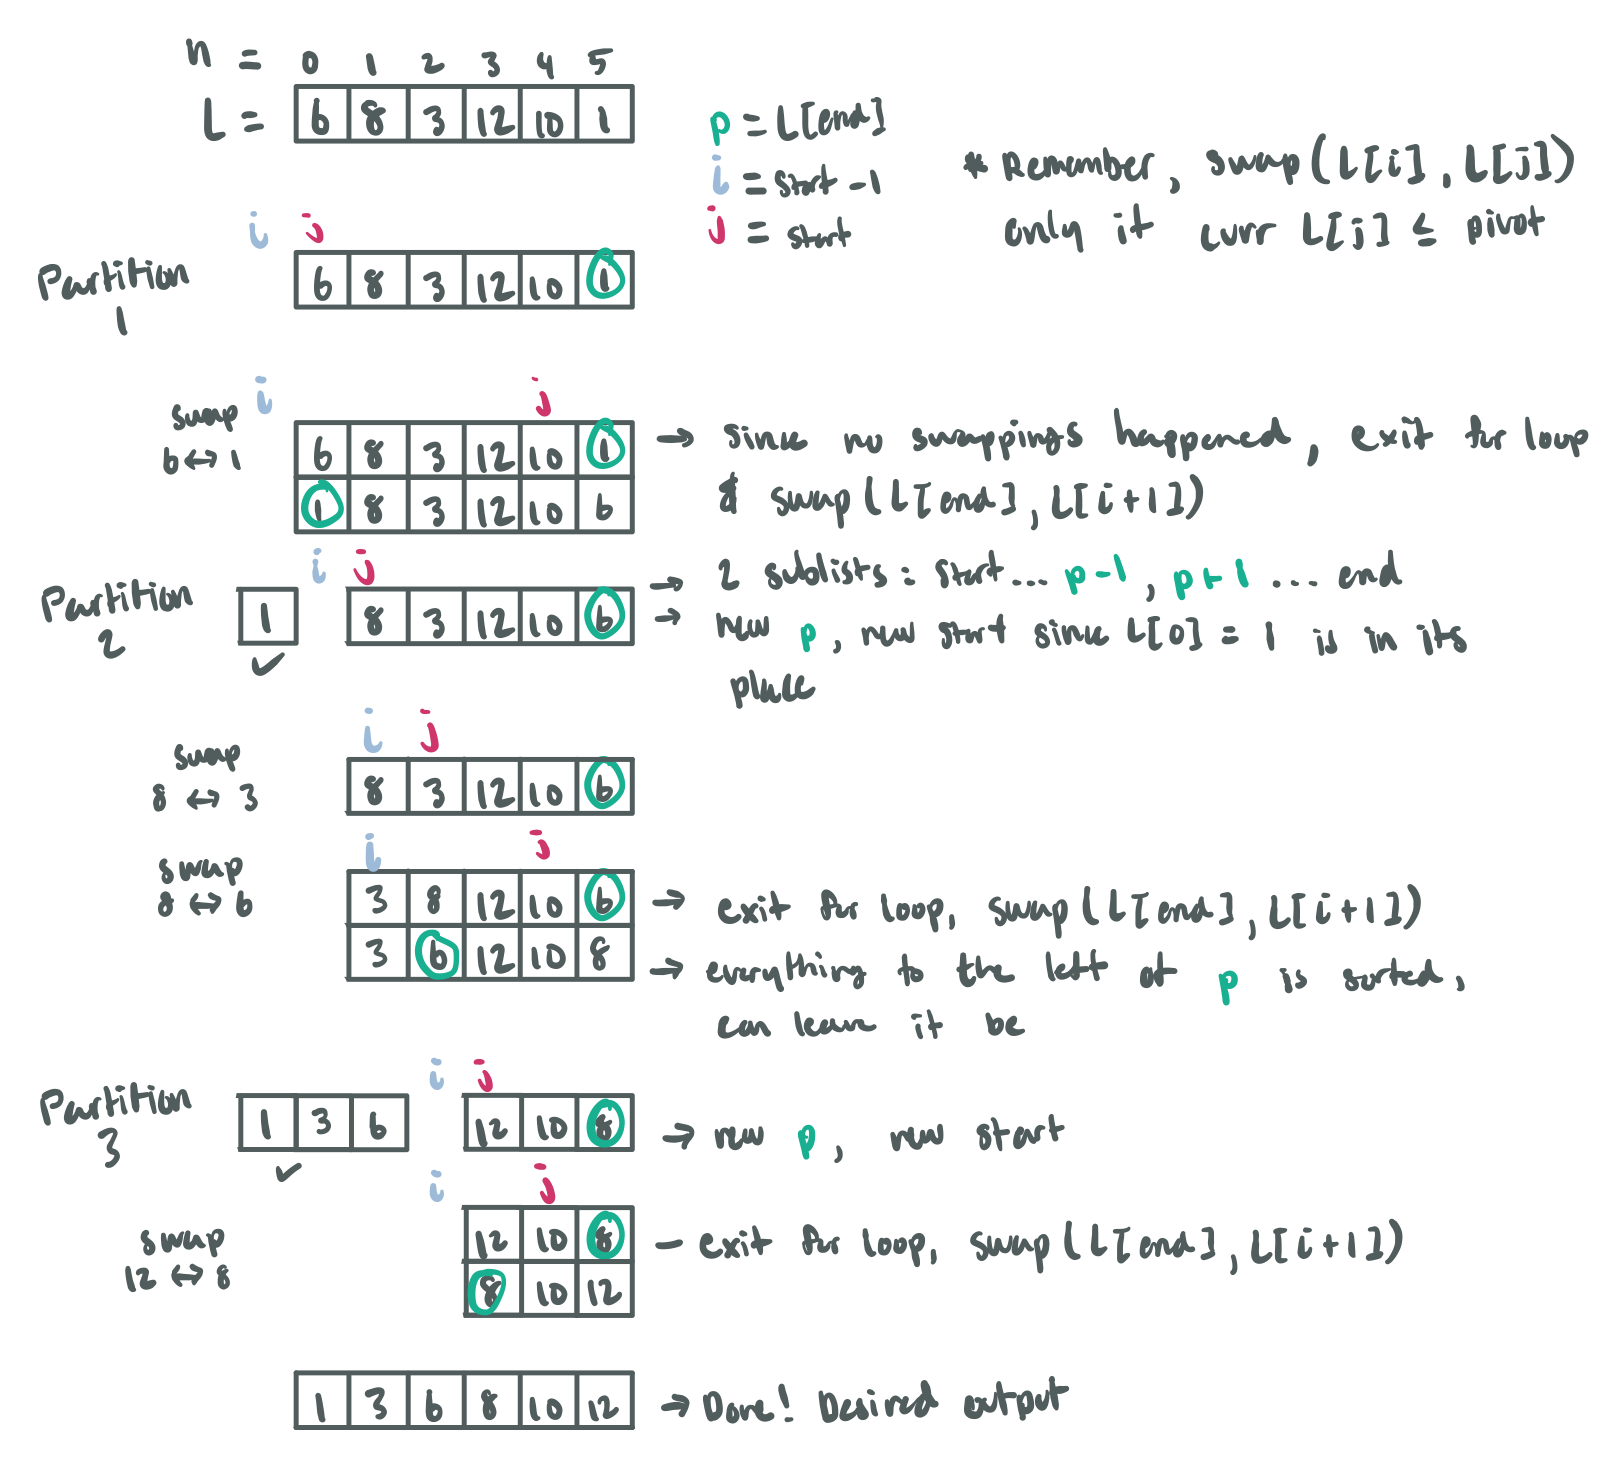
\includegraphics[width=\textwidth]{QuickSort.png}
        \caption{QuickSort following main algorithm}
    \end{center}
\end{figure}
%----Time Complexity----%
\subsubsection{Time Complexity}
\begin{definition}
    \textit{Time Complexity}
    \begin{itemize}
        \item \textbf{B.C}:
        \begin{itemize}
            \item \textbf{partition()}: $\Theta(n)$, B.C when partition creates two equal sublists (or when their lengths differ by 1)
            \item \textbf{sublists}: sizes of $n/2$ and $n/2$
            \item \textbf{Quick-Sort}: $\Theta(n log(n))$, similar to binary search
        \end{itemize} 
        \item \textbf{W.C}:
        \begin{itemize}
            \item \textbf{partition()}: $\Theta(n)$, when list is already sorted (either ascending or descending)
            \item \textbf{sublists}: sizes of $n-1$ and 0 - since one of the lists is empty, recursive call is $O(1)$, other is repeated $n-1$ times
            \item \textbf{Quick-Sort}: $\Theta(n^2)$
        \end{itemize}
    \end{itemize}
\end{definition}
%----Correctness----%
\subsubsection{Correctness}
\begin{definition}
    \textit{Loop Invariant and Mathematical Induction}
    \begin{itemize}
        \item \textbf{Partition}
        \begin{itemize}
            \item \textbf{\textit{Initialization}}
            \begin{itemize}
                \item Before the 1st iteration, $i_0=start-1,j_0=start$
                \begin{enumerate}
                    \item $L[start...i_0]$ is empty
                    \item $L[i_0+1...j_0]$ is a singleton
                \end{enumerate}
                \item Hence, LI is vacuously true
            \end{itemize}
            \item \textbf{\textit{Maintenance}}
            \begin{itemize}
                \item Assume LI is correct before iteration \textit{k}. That is,
                \begin{enumerate}
                    \item $\forall y\in L[start...i_{k-1}], y.key \leq p.key$ and
                    \item $\forall z\in L[i_{k-1}+1...j_{k-1}],z.key>p.key$ 
                \end{enumerate}
                \item In this iteration, if $L[j_k].key\leq p.key,i_k=i_{k-1}+1$, swap $L[j_k],L[i_k]$
                \begin{itemize}
                    \item That is, $\forall y\in L[start...i_{k}], y.key \leq p.key$ and
                    \item $\forall z\in L[i_{k}+1...j_{k}],z.key>p.key$ 
                \end{itemize}
                \item On the other hand, if $L[j_k].key>p.key,i_k=i_{k-1}$
                \begin{itemize}
                    \item That is, $\forall y\in L[start...i_{k}], y.key \leq p.key$ and
                    \item $\forall z\in L[i_{k}+1...j_{k}],z.key>p.key$ 
                \end{itemize}
                \item Both hold, hence LI holds for every iteration
            \end{itemize}
            \item \textbf{\textit{Termination}}
            \begin{itemize}
                \item Last iteration is when $j=end-1$
                \item That is, for some \textit{i}, $(start-1)\geq i \geq end-1$
                \begin{enumerate}
                    \item $\forall y\in L[start...i], y.key \leq p.key$, and
                    \item $\forall z\in L[i+1...end-1],z.key>p.key$
                \end{enumerate}
                \item Last step of the algorithm is to swap $L[end], L[i+1]$, partitioning L into $L[start...i+1]$ and $L[i+2...end]$, where \textit{pivot} is at index $i+1$
                \item Algorithm returns \textit{pivot}, hence it always terminates
            \end{itemize}
        \end{itemize}
        \item \textbf{QuickSort}
        \begin{itemize}
            \item \textbf{\textit{Claim}}: Quick-Sort sorts any list $L[i...j]$ of size $j-i+1=n\geq 0$
            \begin{proof}
                By mathematical induction
                \begin{itemize}
                    \item \textit{\textbf{Inductive Hypothesis}}: Assume Quick-Sort(L, i, j) sorts $L[i...j]$ of size $j-i+1=k$ and $0\leq k<n$
                    \item \textit{\textbf{Inductive Claim}}: Quick-Sort(L, l, m) sorts $L[l...m]$ of size $m-l+1=k+1$. Let \textit{p} be the pivot for $L[l...m]$
                    \begin{itemize}
                        \item Both L[left] and L[right] are sorted by IH
                        \item Partition correctness guarantees that all values in L[left] are $\leq p$ and values in L[right] $>p$
                        \item Hence, Quick-Sort sorts any list of size $n\geq 0$
                    \end{itemize} 
                \end{itemize}
            \end{proof}
        \end{itemize}
    \end{itemize}
\end{definition}
\newpage
%-----------------------------------------------------------------------------------%
%Searching%
\section{Searching}
%--Linear Search--%
\subsection{Linear Search}
%----Algorithm----%
\subsubsection{Algorithm}
\begin{lstlisting}
    // Unsorted List
    public int contains(T item) {
        int i = 0;
        while (i < this.size) {
            if (item.compareTo(this.list[i]) == 0) {
                return i;
            }
            i++;
        }
        return -1;
    }
    // Sorted List
    public int contains(T item) {
        int i = 0;
        while (i < this.size) {
            if (item.compareTo(this.list[i]) == 0) {
                return i;
            } else if (item.compareTo(list[i]) > 0) {
                return -1;
            } else {
                i++;
            }
        }
        return -1;
    }
\end{lstlisting}
%----Time Complexity----%
\subsubsection{Time Complexity}
\begin{definition}
    \textit{Time Complexity}
    \begin{itemize}
        \item \textbf{Unsorted List}
        \begin{itemize}
            \item \textbf{B.C}: $\Theta(1)$, \textit{x} is the first element in the list
            \item \textbf{W.C}: $\Theta(n)$, \textit{x} is not in the list or while loop iterates exactly \textit{n} times 
        \end{itemize}
        \item \textbf{Sorted List}
        \begin{itemize}
            \item \textbf{B.C}: $\Theta(1)$, \textit{x} is the first element in the list
            \item \textbf{W.C}: $O(n)$, \textit{x} is not in the list or while loop iterates exactly \textit{n} times
        \end{itemize}
    \end{itemize}
\end{definition}
%----Correctness----%
\subsubsection{Correctness}
\begin{definition}
    \textit{Loop Invariant}
    \begin{itemize}
        \item \textit{\textbf{Initialization}}
        \begin{itemize}
            \item Before the first iteration, $k=0$, $[0,0]$ is empty, and $list[i].key \neq item.key$
            \item LI holds true
        \end{itemize}
        \item \textit{\textbf{Maintenance}}
        \begin{itemize}
            \item If the item is found in iteration $k-1$, algorithm terminates, returning $k-1$ as required
            \item So, assume item was not found in the previous iteration and there is a $k^{th}$ iteration
            \item Assume LI is true before the $k^{th}$ iteration
            \item \textbf{Case 1}: Since there is a $k^{th}$ iteration, $\forall i \in[0,k]: list[i].key\neq item.key$
            \item \textbf{Case 2}: When $list[k].key\neq item.key$
            \item \textbf{1} and \textbf{2} $\rightarrow \forall i \in[0,k+1]: list[i].key\neq item.key$
            \item Otherwise, if in the $k^{th}$ iteration, $list[k].key = item.key$, there will be no $k^{th}+1$ iteration since algorithm terminates, returning \textit{k} as required
            \item Hence, LI holds true at the end of the $k^{th}$ iteration
        \end{itemize}
        \item \textit{\textbf{Termination}}
        \begin{itemize}
            \item While loop terminates if
            \begin{itemize}
                \item \textbf{1.} $list[i].key=item.key$, where \textit{i} is returned as required
                \item \textbf{2.} $i=list.size$, -1 is returned as required
            \end{itemize}
            \item Hence, LI holds true when algorithm terminates
        \end{itemize}
    \end{itemize}
\end{definition}
\newpage
%-----------------------------------------------------------------------------------%
%--Binary Search--%
\subsection{Binary Search}
Only works for sorted lists, typically with an array-implementation
%----Algorithm----%
\subsubsection{Algorithm}
\begin{lstlisting}
    // Recursive
    Binary-Search(item x, item[] L, int low, int high) {
        if (low > high) {
            return - 1;
        }
        int mid = (low + high)/2;
        if (x.key == L[mid].key) {
            return mid;
        } else if (x.key < L[mid].key) {
            return Binary-Search(x, L, low, mid - 1);
        } else {
            return Binary-Search(x, L, mid + 1; high);
        }
    }
    // Iterative
    Binary-Search(item x, item[] L) {
        int low = 0;
        int high = L.size - 1;
        
        while (low <= high) {
            int mid = (low + high)/2;
            if (x.key == L[mid].key) {
                return mid;
            } else if (x.key < L[mid].key) {
                high = mid - 1;
            } else {
                low = mid + 1;
            }
        }
        return -1;
    }
\end{lstlisting}
%----Time Complexity----%
\subsubsection{Time Complexity}
Both iterative and recursive are of $O(\log(n))$
%----Correctness----%
\subsubsection{Correctness}
\textit{Loop Invariant}
\begin{itemize}
    \item Two clauses to satisfy
    \begin{enumerate}
        \item $1\leq low\leq high\leq L.size$
        \item If our key is in L, then there is some target of the key where L[target] = key. Then, $1\leq target\leq L.size$ 
        and $low\leq target\leq high$, hence we are searching through the correct range for key
    \end{enumerate}
    \item \textit{\textbf{Initialization}}
    \begin{itemize}
        \item Since our L is at least size 1, clause 1 holds
        \item Suppose key is in L. This mean that $1\leq target\leq L.size-1$ holds true 
    \end{itemize}
    \item \textit{\textbf{Maintenance}}
    \begin{itemize}
        \item \textit{BC 1}: $L[mid] < key$
        \begin{itemize}
            \item We search through elements in $L[mid+1,high]$ since key is larger than mid
            \item We know that key is $\leq high$ by IH, otherwise it would violate the precondition
            \item Hence, key is in $L[mid+1,high]$
        \end{itemize}
        \item \textit{BC 2}: $L[mid] > key$ (Similar to above case)
        \item \textit{BC 3}: $L[mid] == key$
        \begin{itemize}
            \item Return mid, as key happened to be in the position mid was in
        \end{itemize}
        \item \textit{BC 1, 2, 3} holds true for all cases, thus we can conclude that LI holds for the $i+1$ iteration, as claimed
    \end{itemize}
    \item \textit{\textbf{Termination}}
    \begin{itemize}
        \item We must prove that if 
        \begin{itemize}
            \item $[low_i,high_i]$ on $i^{th}$ iteration and
            \item $[low_{i+1},high_{i+1}]$ on iteration $i+1$,
        \end{itemize}
        \item $high_{i+1}-low_{i+1}<high_{i}-low_{i}$
        \item By each condition, we will perform integer division
        \item Hence, the array gets smaller on every iteration of the loop, eventually leading to termination
    \end{itemize}
\end{itemize}
\newpage
%-----------------------------------------------------------------------------------%
%Graph Traversal%
\section{Graph Traversal}
%--Depth-first Search--%
\subsection{Depth-First Search}
\begin{itemize}
    \item Uses stack to explore a branch as far as possible before backtracking
    \item Backtracking achieved by popping from stack
    \item \textbf{IMPORTANT}: For this exam, push vertices onto the stack such that the vertex with the smallest ID (numerical value) 
    is on the top
    \begin{itemize}
        \item e.g. Adjacency List for Node 0: AL[0]$\rightarrow$[1$\rightarrow$2] or AL[0]$\rightarrow$[2$\rightarrow$1]
        \item will be pushed onto the stack like the following:
        \item (TOS) <1, 2> (BOS)
    \end{itemize}
\end{itemize}
%----Algorithm----%
\subsubsection{Algorithm}
\begin{lstlisting}
    // Iterative 
    Queue<Integer> DFS(Graph g, int start) {
        Stack<Integer> stack = new Stack<>();
        Queue<Integer> queue = new Queue<>();
        Set<Integer> visited = new Set<>();

        stack.push(start);
        while (!stack.isEmpty()) {
            int u = stack.pop();
            visited.add(u);
            queue.enqueue(u);
            for (int v : G.adjacencyList[u]) {
                if (!visited.contains(v)) {
                    stack.push(v);
                }
            }
        }
        return queue;
    }
\end{lstlisting}
%----Time Complexity----%
\subsubsection{Time Complexity}
%----Correctness----%
\subsubsection{Correctness}
%----Applications----%
\subsubsection{Applications}
\begin{itemize}
    \item \textbf{Cycle Detection}: Any time you encounter a new edge that points an already visited vertex then you have a cycle
    \item \textbf{Topological Sort}: applies to directed acyclic graph (no cycles)
    \begin{itemize}
        \item Finds a valid order to execute tasks in a directed cyclic graph
    \end{itemize}
\end{itemize}
\newpage
%-----------------------------------------------------------------------------------%
%--Breadth-first Search--%
\subsection{Breadth-First Search}
\begin{itemize}
    \item Visit vertices by depth, meaning we visit every single vertex
    \item Uses a queue to explore each level before moving onto the next
    \item Backtracks by dequeueing from tmpQ
    \item \textbf{IMPORTANT}: For this exam, enqueue vertices into tmpQ such that vertices with smallest ID are towards the front of the queue
\end{itemize}
%----Algorithm----%
\subsubsection{Algorithm}
\begin{lstlisting}
    Queue<Integer> BFS(Graph g, int start) {
        Queue<Integer> queue = new Queue<>();
        Queue<Integer> tmpQ = new Queue<>();
        Set<Integer> visited = new Set<>();

        tmpQ.enqueue(start);
        while (!tmpQ.isEmpty()) {
            int u = tmpQ.dequeue();
            visited.add(u);
            queue.enqueue(u);
            for (int v : g.adjacencyList[u]) {
                if (!visited.contains(v)) {
                    tmpQ.enqueue(v);
                }
            }
        }
        return queue;
    }
\end{lstlisting}
%----Time Complexity----%
\subsubsection{Time Complexity}
%----Correctness----%
\subsubsection{Correctness}
%----Applications----%
\subsubsection{Applications}
\textbf{Spanning Tree}
\begin{figure}[H]
    \begin{center}
        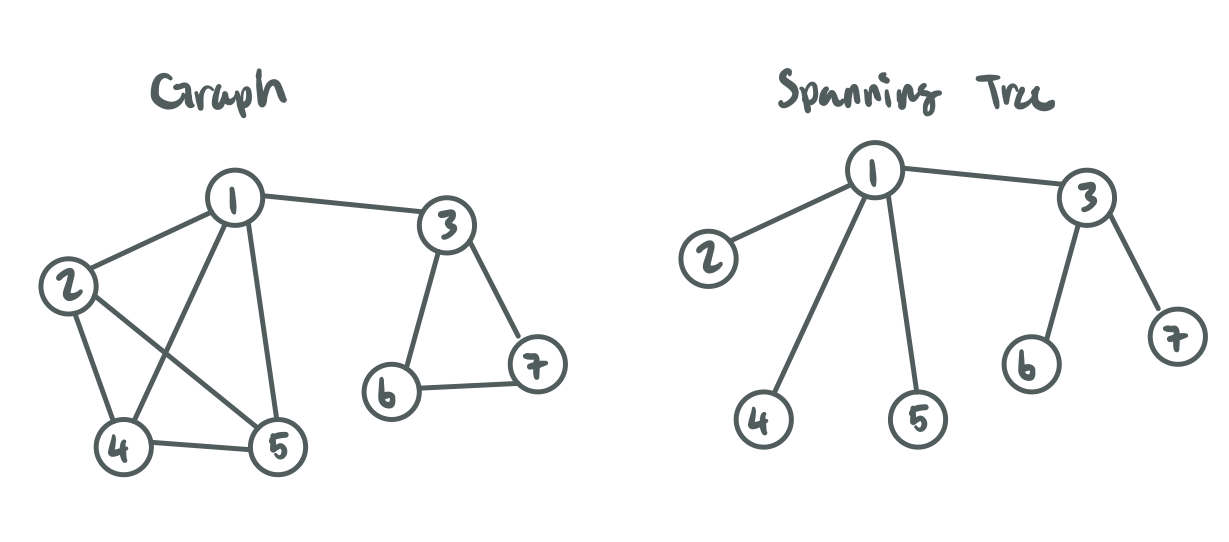
\includegraphics[width=\textwidth]{SpanningTree.png}
    \end{center}
\end{figure}
\newpage
%-----------------------------------------------------------------------------------%
\end{document}
